% Document Type Management
    \documentclass{book}
    \usepackage[utf8]{inputenc}
    \usepackage[english]{babel}
     
 
 % Packages for Bibliographic Management
    \usepackage{biblatex}
    \usepackage{csquotes}
    \addbibresource{references.bib}

% AMS Packages
    \usepackage{amsfonts}
    \usepackage{amssymb}
    \usepackage{amsmath}
    \usepackage{amsthm}
    \usepackage{esvect}
    \usepackage{blindtext}


% Images Management Packages
    \usepackage{tcolorbox}
    \usepackage{graphicx}
    \graphicspath{ {images/} }


% Packages to Draw Images
    \usepackage{float}
    \usepackage{tikz}
    \usetikzlibrary{shapes,backgrounds}
    \usetikzlibrary{positioning}


% Custom Section Labels   
        \newtheorem{theorem}{Theorem}[section]
        \newtheorem{conjecture}[theorem]{Conjecture}
        \newtheorem{corollary}{Corollary}[theorem]
        \newtheorem{lemma}[theorem]{Lemma}

    \theoremstyle{definition}
        \newtheorem{definition}{Definition}[section]
        \newtheorem{example}{Example}[definition]
        \newtheorem{entry}{Entry}[definition]
 
    \theoremstyle{remark}
        \newtheorem{remark}{Remark}





% Custom Chapters and Sections
    \usepackage{titlesec}
    
    \renewcommand\contentsname{Table of Contents}
    \titleformat{\chapter}[display]
      {\bfseries\large}
      {\filleft\MakeUppercase{\chaptertitlename} \large\thechapter}
      {2ex}
      {\titlerule\vspace{2ex}\filleft}
    \titleformat{name=\chapter,numberless}[display]
      {\bfseries\large}
      {\titlerule}
      {-7ex}
      {\filleft\MakeUppercase}[\vspace{5ex}]
    \titlespacing*{\chapter}{0pt}{120pt}{6pt}


% Custom Commands '
    \newcommand{\bb}[1]{\mathbb{#1}}
    \newcommand{\cc}[1]{\mathcal{#1}}
    \newcommand{\ovec}{\big \langle}
    \newcommand{\cvec}{\big \rangle}
    \newcommand{\m}{\cdot}



\begin{document}

\begin{titlepage}
    \begin{center}
        \vspace*{1cm}
        
        \textbf{MATHEMATICAL PROOF STRUCTURES}
        
        \vspace{0.5cm}
        Logic - Set Theory - Number Theory - Linear Algebra
        
        \vspace{1.5cm}
        
        \textbf{Vernon V. Lallman}
        
        \vfill
        
%        A thesis presented for the degree of\\
%        Doctor of Philosophy
        
        \vspace{0.8cm}
        
        
\includegraphics[width=0.4\textwidth]{university}
        
        Mathematics Department\\
        State University of New York \\
        Geneseo\\
        \date{\today}
        
    \end{center}
\end{titlepage}

\tableofcontents


\newpage
\chapter{TOPICS IN LOGIC}
\section{Statements and Conditional Statements}

\begin{definition}
Statement \\

A statement is a declarative sentence that is either true or false but not both. \\
\end{definition}

\begin{definition}
Conditional Statements

A Conditional Statement is a statement that can be written in the form {\bf If $P$, then $Q$}, where $P$ and $Q$ are sentences. For this conditional statement, $P$ is called the {\bf hypothesis} and $Q$ is called the conclusion. \\

\begin{minipage}{1\textwidth}
1. If $P$ is true and $Q$ is true, then $P$ implies $Q$ is a true \\
2. If $P$ is true and $Q$ is false, then $P$ implies $Q$ is a false \\
3. If $P$ is false and $Q$ is true, then $P$ implies $Q$ is a true \\
4. If $P$ is false and $Q$ is false, then $P$ implies $Q$ is a true \\
\end{minipage}
\end{definition}

\begin{definition}
Even and Odd Integers \\

An integer $a$ is an {\bf even integer} provided tha there exisits an integer $n$ such that $a = 2n$. An integer $a$ is an {\bf odd integer} provided there exists an integer $n$ such that $a = 2n + 1$
\end{definition}


\begin{definition}
Closure Properties of Number Systems

Three of the basic properties of the integers are that that the set $\bb{Z}$ is a {\bf closed under addition}, the set $\bb{Z}$ is {\bf closed under multiplication}, and the set of integers is {\bf closed under subtraction}. This means that: \\

$\bb{Z}$ Closed Under Addition: If $x$ and $y$ are integers, then $x+y$ is an integer. \\
 
$\bb{Z}$ Closed Under Multiplication: If $x$ and $y$ are integers, then $x*y$ is an integer. \\

$\bb{Z}$ Closed Under Subtraction: If $x$ and $y$ are integers, then $x+y$ is an integer. \\

\end{definition}

\newpage
\section{Mathematical Proof Structures}

\begin{definition}
Mathematical Definition

A mathematical definition is an agreement that a partiular word or phrase will stand for some object, property, or other concept that we expect to refer to often. In many elementary proofd, the answer to the question: {\bf How do we prove a certain proposition}, is often answered by means of a definition. 
\end{definition}


\begin{definition}
Mathematical Proof \\

A mathematical proof is a convincing argument (within the accepted standards of the mathematical community) that a certain mathematical statement is necessarily true. A proof generally uses deductive reasoning and logic but also contains some amount of ordinary language. Here are some general guidelines for writing proofs: \\
1. Begin with a carefully worded statement of the theorem or result to be proven \\
2. Begin the proof with a statement of your assumptions \\
3. Use the pronoun "we" \\
4. Use italcs for variables when using a word processor \\
5. Display important equations and mathematical expressions \\
6. Tell the reader when the proof has been completed \\
\end{definition}







\newpage
\section{Logical Operators}

1. The {\bf conjunction} of statements $P$ and $Q$ is the statement $P \wedge Q$. The Truth Table is as follows: 

A logical operator (or connective) on mathematical statements is a word or combination of words that combines one or more mathematical statements into a compound (mathematical) statement. The logical operators are: \\

\begin{definition}
Conjunction \\

The {\bf conjunction} of statements with variables $P$ and $Q$ is the statement $P \wedge Q$. The truth table is as follows: \\
\begin{center}
\begin{tabular}{|c|c|c|}
\hline 
P & Q & $P \wedge Q$ \\ 
\hline 
T & T & T \\ 
\hline 
T & F & F \\ 
\hline 
F & T & F \\ 
\hline 
F & F & F \\ 
\hline 
\end{tabular} 
\end{center}
\end{definition}


\begin{definition}
Inclusive Or \\

The {\bf inclusive or} of statements with variables $P$ and $Q$ is the statement $P \vee Q$. The truth table is as follows: \\
\begin{center}
\begin{tabular}{|c|c|c|}
\hline 
P & Q & $P \vee Q$ \\ 
\hline 
T & T & T \\ 
\hline 
T & F & T \\ 
\hline 
F & T & T \\ 
\hline 
F & F & F \\ 
\hline 
\end{tabular} 
\end{center}
\end{definition}

\begin{definition}
Exclusive Or

The {\bf exclusive or} of statements with variables $P$ and $Q$ is the statement $P \oplus Q$. The truth table is as follows: \\
\begin{center}
\begin{tabular}{|c|c|c|}
\hline 
P & Q & $P \oplus Q$ \\ 
\hline 
T & T & F \\ 
\hline 
T & F & T \\ 
\hline 
F & T & T \\ 
\hline 
F & F & F \\ 
\hline 
\end{tabular} 
\end{center}
\end{definition}


\begin{definition}
Negation \\

The {\bf negation} of statements with variable $P$ is the statement $\neg P$. The Truth Table is as follows: \\
\begin{center}
\begin{tabular}{|c|c|c|}
\hline 
P & $\neg P$ \\ 
\hline 
T & F \\ 
\hline 
F & T \\ 
\hline 
\end{tabular} 
\end{center}
\end{definition}


\begin{definition}
Implication \\

The {\bf implication} of statements with variables $P$ and $Q$ is the statement $P \to Q$. The Truth Table is as follows: \\
\begin{center}
\begin{tabular}{|c|c|c|}
\hline 
P & Q & $P \to Q$ \\ 
\hline 
T & T & T \\ 
\hline 
T & F & F \\ 
\hline 
F & T & T \\ 
\hline 
F & F & T \\ 
\hline 
\end{tabular} 
\end{center}
\end{definition}

\begin{definition}
Converse Statement \\

The {\bf converse} of the conditional statement $P \to Q$ is the conditional statement $Q \to P$
\end{definition}

\begin{definition}
Contrapositive Statement \\

The {\bf contrapositive} of the conditional statement $P \to Q$ is the conditional statement $\neg Q \to \neg P$
\end{definition}


\begin{definition}
Concept of Necessary Condition \\
A condition $P$ is said to be necessary for a condition $Q$, if (and only if) the falsity (/nonexistence /non-occurrence) [as the case may be] of $P$ guarantees (or brings about) the falsity (/nonexistence /non-occurrence) of $Q$. \\

\begin{center}
\begin{tabular}{|c|c|c|}
\hline 
P & Q & $P Necessary Q$ \\ 
\hline 
T & T & T \\ 
\hline 
T & F & T \\ 
\hline 
F & T & F \\ 
\hline 
F & F & T \\ 
\hline 
\end{tabular} 
\end{center}

\end{definition}

\begin{definition}
Concept of Sufficient Condition \\
A condition $P$ is said to be sufficient for a condition $Q$, if (and only if) the truth (/existence /occurrence) [as the case may be] of $P$ guarantees (or brings about) the truth (/existence /occurrence) of $Q$.

\begin{center}
\begin{tabular}{|c|c|c|}
\hline 
P & Q & $P Sufficient Q$ \\ 
\hline 
T & T & T \\ 
\hline 
T & F & F \\ 
\hline 
F & T & T \\ 
\hline 
F & F & T \\ 
\hline 
\end{tabular} 
\end{center}
\end{definition}


\begin{definition}
Converse Statement of a Necessary or Sufficient Implication \\

The converse of the conditional statement {\bf $P$ is sufficient for $Q$} is the conditional statement {\bf $Q$ is necessary $P$}. While the converse of the conditional statement {\bf $Q$ is necessary for $P$} is the conditional statement {\bf $P$ is sufficient for $Q$}.
\end{definition}


\begin{definition}
Contrapositive Statement of a Necessary or Sufficient Implication \\

The contrapositive of the conditional statement {\bf $P$ is sufficient for $Q$} is the conditional statement {\bf $\neg Q$ is necessary for  $\neg P$}. While the contrapositive of the conditional statement {\bf $Q$ is necessary for $P$} is the conditional statement {\bf $\neg P$ is sufficient for $\neg Q$}. 
\end{definition}



\begin{definition}
Equivalence of Necessary and Sufficient Conditions \\
The conditional statement {\bf $P$ is sufficient for $Q$} is equivalent to the statement {\bf the condition $Q$ is necessary for $P$}. While, the statement {\bf $P$ is a necessary for $Q$} is equivalent to the statement {\bf $Q$ is sufficient for $P$}. \\
\end{definition}


%\begin{figure}
%	\wedgetion{Graph of inter-relationships between common 4-sided polygons}
%	\centering
%	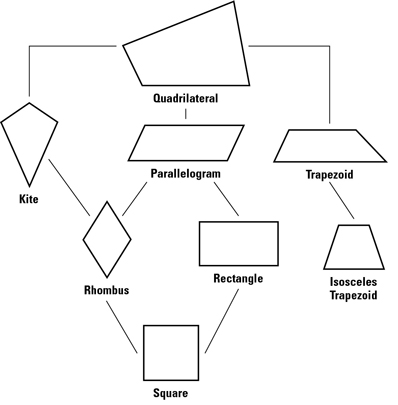
\includegraphics{4-Sided-Polygon}
%\end{figure}

\newpage
\begin{tcolorbox}
\begin{definition}
Quadrilateral 

A polygon is a quadrilateral if and only if it's a plane figure with four straight sides and angles. 
\end{definition}


\begin{definition}
Kite 

A quadrilateral is a kite if and only if it has the following properties: \\
1. Pairs of sides are congruent by definition \\
2. Only One pair of diagonally opposite angles is equal
3. Only one diagonal bisect the other angle \\
4. The diagonals are perpendicular bisectors of each other \\
\end{definition}


\begin{definition}
Parallelogram 

A quadrilateral is a parallelogram if and only if it has the following properties: \\
1. Parallel sides
2. Opposite angles are congruent 
3. Consecutive angles are supplementary
\end{definition}


\begin{definition}
Rhombus 

A parallelogram is a rhombus if and only if it has the following properties: \\
1. All the properties of a parallelogram \\
2. All sides are congruent by definition \\
3. The diagonals bisect the angles \\
4. The diagonals are perpendicular bisectors of each other \\
\end{definition}


\begin{definition}
Rectangle 

A parallelogram is a rectangle if and only if it has the following properties: \\
1. All the properties of a parallelogram \\
2. All angles are right angles by definition \\
3. The diagonals are congruent \\
\end{definition}


\begin{definition}
Square

A parallelogram is a square if and only if it has the following properties: \\
1. All the properties of a rhombus \\
2. All the properties of a rectangle apply \\
\end{definition}
\end{tcolorbox}

\newpage
\begin{definition}
4-Sided Polygon Theorems Examples \\

Examples of converse statements with necessary conditions that are not sufficient on the left and sufficient conditions that are not necessary on the right: \\

1. {\bf A Rectangle and Rhombus are necessary conditions of a plane figure to be a Square} is the converse ofdd the statement {\bf A Square is a sufficient condition for a plane figure to be a either a Rectangle or a Rhombus} \\


2. {\bf A Parallelogram is a necessary condition for a plane figure to be a a Rectangle} is the converse of the statement {\bf A Rectangle is a sufficient condition for a plane figure to be a Parallelogram}\\

3. {\bf A Kite or a Parallelogram is a necessary condition for a plane figure to be Rhombus} is the converse of the statement {\bf A Rhombus is a sufficient condition for a plane figure to be either a Kite or Parallelogram}\\

4. {\bf A Quadrilateral is a necessary condition for a plane figure to be a Kite} is the converse of the statement {\bf A Kite is a sufficient condition for a plane figure to to be a Quadrilateral} \\

5. {\bf A Quadrilateral is a necessary condition for a plane figure to be a Parallelogram} is the converse of the statement {\bf A Parallelogram is a sufficient condition for a plane figure to be Quadrilateral} \\
\end{definition}

\newpage
\begin{definition}
Conjunctive and Disjunctive Statements involving Necessary and Sufficient Conditions \\

The relationship between the two conditions must be exactly one of the following four possibilities: \\
1. $nec \wedge suf$ CASE: {\bf $[P$ necessary $Q] \wedge [P$ sufficient $Q]$} \\
\begin{center}
\begin{tabular}{|c|c|c|c|c|}
\hline 
P & Q & P nec Q & P suf Q & $[P$ nec $Q] \wedge [P$ suf $Q]$  \\ 
\hline 
T & T & T & T & T\\ 
\hline 
T & F & T & F & F\\ 
\hline 
F & T & F & T & F\\ 
\hline 
F & F & T & T & T\\ 
\hline 
\end{tabular} 
\end{center}

2. $nec \vee suf$ CASE: {\bf $[P$ necessary $Q] \vee [P$ sufficient $Q]$} \\
\begin{center}
\begin{tabular}{|c|c|c|c|c|}
\hline 
P & Q & P nec Q & P suf Q & $[P$ nec $Q] \wedge [P$ suf $Q]$  \\ 
\hline 
T & T & T & T & T\\ 
\hline 
T & F & T & F & T\\ 
\hline 
F & T & F & T & T\\ 
\hline 
F & F & T & T & T\\ 
\hline 
\end{tabular} 
\end{center}

3. $\neg nec \wedge suf$ CASE: {\bf $\neg[P$ necessary $Q] \wedge [P$ sufficient $Q]$} \\
\begin{center}
\begin{tabular}{|c|c|c|c|c|}
\hline 
P & Q & P nec Q & P suf Q & $\neg[P$ nec $Q] \wedge [P$ suf $Q]$  \\ 
\hline 
T & T & T & T & F\\ 
\hline 
T & F & T & F & F\\ 
\hline 
F & T & F & T & T\\ 
\hline 
F & F & T & T & F\\ 
\hline 
\end{tabular} 
\end{center}


4. $nec \wedge \neg suf$ CASE: {\bf $[P$ necessary $Q] \wedge \neg[P$ sufficient $Q]$} \\
\begin{center}
\begin{tabular}{|c|c|c|c|c|}
\hline 
P & Q & P nec Q & P suf Q & $\neg[P$ nec $Q] \wedge \neg[P$ suf $Q]$  \\ 
\hline 
T & T & T & T & F\\ 
\hline 
T & F & T & F & T\\ 
\hline 
F & T & F & T & F\\ 
\hline 
F & F & T & T & F\\ 
\hline 
\end{tabular} 
\end{center}

5. $\neg nec \vee suf$ CASE: {\bf $\neg[P$ necessary $Q] \vee [P$ sufficient $Q]$} \\
\begin{center}
\begin{tabular}{|c|c|c|c|c|}
\hline 
P & Q & P nec Q & P suf Q & $\neg[P$ nec $Q] \vee [P$ suf $Q]$  \\ 
\hline 
T & T & T & T & T\\ 
\hline 
T & F & T & F & F\\ 
\hline 
F & T & F & T & T\\ 
\hline 
F & F & T & T & T\\ 
\hline 
\end{tabular} 
\end{center}


6. $nec \vee \neg suf$ CASE: {\bf $[P$ necessary $Q] \vee \neg[P$ sufficient $Q]$} \\
\begin{center}
\begin{tabular}{|c|c|c|c|c|}
\hline 
P & Q & P nec Q & P suf Q & $[P$ nec $Q] \vee \neg[P$ suf $Q]$  \\ 
\hline 
T & T & T & T & T\\ 
\hline 
T & F & T & F & T\\ 
\hline 
F & T & F & T & F\\ 
\hline 
F & F & T & T & T\\ 
\hline 
\end{tabular} 
\end{center}


7. $\neg(nec \wedge suf)$ CASE: {\bf $\neg([P$ necessary $Q] \wedge [P$ sufficient $Q])$} \\
\begin{center}
\begin{tabular}{|c|c|c|c|c|}
\hline 
P & Q & P nec Q & P suf Q & $\neg[P$ nec $Q] \vee \neg[P$ suf $Q]$  \\ 
\hline 
T & T & T & T & F\\ 
\hline 
T & F & T & F & T\\ 
\hline 
F & T & F & T & T\\ 
\hline 
F & F & T & T & F\\ 
\hline 
\end{tabular} 
\end{center}

8. $\neg(nec \vee suf)$ CASE: {\bf $\neg([P$ necessary $Q] \vee [P$ sufficient $Q])$} \\
\begin{center}
\begin{tabular}{|c|c|c|c|c|}
\hline 
P & Q & P nec Q & P suf Q & $\neg[P$ nec $Q] \wedge \neg[P$ suf $Q]$  \\ 
\hline 
T & T & T & T & F\\ 
\hline 
T & F & T & F & F\\ 
\hline 
F & T & F & T & F\\ 
\hline 
F & F & T & T & F\\ 
\hline 
\end{tabular} 
\end{center} 
\end{definition}

\begin{definition}
Synonyms of Implication

\begin{center}
\begin{tabular}{|c|c|}
\hline 
FORM 1 & FORM 2 \\ 
\hline 
If $P$, then $Q$ & $P$ if $Q$ \\ 
\hline 
$P$ implies $Q$ & $Q$ is necessary for $P$ \\ 
\hline 
$P$ only if $Q$ & $Q$ is true whenever $P$ is true \\ 
\hline 
$P$ is sufficient for $Q$ & • \\ 
\hline 
Whenever $P$ is true, Q is true & • \\ 
\hline 
$Q$ if $P$ & • \\ 
\hline 
\end{tabular} 
\end{center}
\end{definition}



\newpage
\section{Logically Equivalent Statements}
\begin{definition}
Logically Equivalent Statement \\

Two expressions are logically equivalent provided that they have the same truth value for all possible combinations of truth values for all variables appearing in the two expressions. In this case, we write $X \equiv Y$ and say that $X$ is logically equivalent to $Y$ \\
\end{definition}

\begin{tcolorbox}
\begin{theorem}
Logical Equivalent Biconditional Statement \\
For the statements $P$, $Q$, and $R$: \\
\begin{tabular}{|c|c|c|}
\hline 
Num & Theorem Name & Logically Equivalent Statements \\ 
\hline 
1 & De Morgan Law & $\neg(P \wedge Q) \equiv \neg P \vee \neg Q$ \\ 
\hline 
2 & De Morgan Law & $\neg(P \vee Q) \equiv \neg P \wedge \neg Q$ \\ 
\hline 
3 & Conditional Statements  & $P \to Q \equiv \neg P \vee Q$ \\ 
\hline 
4 & Conditional Statements & $\neg (P \to Q) \equiv P \wedge \neg Q$ \\ 
\hline 
5 & Conditional Statements & $P \to Q \equiv \neg Q \to \neg P$ \\ 
\hline 
6 & Biconditional Statements & $P \leftrightarrow Q \equiv (P \to Q) \wedge (Q \to P)$ \\ 
\hline 
7 & Double Negation & $\neg(\neg P) \equiv P$ \\ 
\hline 
8 & Distribution Law & $P \vee (Q \wedge R) \equiv (P \vee Q) \wedge (P \vee R)$ \\ 
\hline 
9 & Distribution Law & $P \wedge (Q \vee R) \equiv (P \wedge Q) \vee (P \wedge R)$ \\ 
\hline 
10 & Conditional with Disjunction & $P \to (Q \vee R) \equiv (P \wedge \neg Q) \to R$ \\ 
\hline 
10 & Conditional with Disjunction & $(P \vee Q) \to R \equiv (P \to R) \wedge (Q \to R)$ \\ 
\hline 
\end{tabular} 
\end{theorem}
\end{tcolorbox}


\newpage
\section{Propositional Logic Repository} 

\begin{example}
Statements \cite[Chap.1, P.C.1.1, Q.1-13]{ted} \\

Which of the following sentences are statements? 
Do not worry about determining whether a statement is true or false; just determine whether each sentence is a statement or not. \\


1. $3+4 = 8$ \\
{\it ANSWER: This is a statement} \\

2. $2*7 + 8 = 22$ \\
{\it ANSWER: This is a statement} \\

3. $(x-1)=\sqrt{x+11}$ \\
{\it ANSWER: This is not a statement since it is not known what $x$ represents} \\

4. $2x+5y=7$ \\
{\it ANSWER: This is not a statement since it is not known what $x$ and $y$ represents} \\

5. There are integers $x$ and $y$ such that $2x +5y =7$ \\
{\it ANSWER: This is a statement} \\

6. There are integers $x$ and $y$ such that $23x +37y =52$ \\
{\it ANSWER: This is a statement} \\

7. Given a line "L" and a point "P" not on a line, there is a unique line through "P" that does not intersect "L" \\
{\it ANSWER: This is a statement} \\

8. $(a+b)^3 = a^3 + 3a^2b + 3ab^2 + b^3$ \\
{\it ANSWER: This is not a statement since it is not known what $a$ and $b$ represents} \\

9. $(a+b)^3 = a^3 + 3a^2b + 3ab^2 + b^3$ for all real numbers $a$ and $b$\\
{\it ANSWER: This is a statement} \\

10. The derivative of $f(x) = sin(x)$ is $f'(x)=cos(x)$ \\
{\it ANSWER: This is not a statement since it is not known what $x$ represents} \\

11. Does the equation $3x^2 - 5x -7 = 0$ have two real number solutions 
{\it ANSWER: This is not a statement it is a question} \\

12. If $ABC$ is a right angle triangle with right angle at vertex $B$, and if $D$ is the midpoint of the hypotenuse, then the line segment connecting vertex $B$ to $D$ is half the length of the hypotenuse. \\
{\it ANSWER: This is a statement} \\

13. There do not exist three integers $x$, $y$ and $z$ such that $x^3 + y^3 = z^3$ \\
{\it ANSWER: This is a statement} \\
\end{example}


\begin{example}
Statements \cite[Chap.1, P.C.1.2, Q.1-4]{ted} \\

Use the technique of exploration to investigate each of the following statements.
Can you make a conjecture as to whether the statement is true or false? Can you determine whether it is true or false? \\


1. $(a+b)^2 = a^2 + b^2$, for all real numbers $a$ and $b$ \\
{\it ANSWER: This conjecture is because $(a+b)^2 = a^2 + 2ab + b^2$} \\

2. There are integers $x$ and $y$ such that $2x + 5y = 41$ \\
{\it ANSWER: This conjecture appears to true because there exists at least one value for $x$ and $y$ that will yield sum $41$} \\

3. If $x$ is an even integer, then $x^2$ is an even integer. \\
{\it ANSWER: This conjecture appears to be true because when square the even integers $2$ and $30$, the solution is an even integer} \\

4. If $x$ and $y$ are odd integers, then $x*y$ is an odd integer \\
{\it ANSWER: This conjecture appears to be true becuase when multiply the odd integers $3$ and $5$, the solution is an odd integer} \\
\end{example}


\begin{example}
Statements \cite[Chap.1, P.C.1.4, Q.1]{ted} \\

Use the technique of exploration to investigate each of the following statements. Can you make a conjecture as to whether the statement is true or false? Can you determine whether it is true or false? \\

\begin{tcolorbox}
    \begin{theorem}
        If $x$ is a positive real number, then $x^2 + 8x$ is a positive real number.
    \end{theorem}
\end{tcolorbox}

{\it NOTE: Although the hypothesis and conclusion of this conditional sentence are not statements, the conditional sentence itself can be considered to be a statement as long as we know what possible numbers may be used for the variable $x$. From the context of this sentence, it seems that we can substitute $0$ for $x$ or a negative real number from $x$ provided that we are willing to work with a false hypothesis in the conditional statement.} \\

1.A. Notice that  if $x=-3$ then $x^2 + 8x = -15$, which is negative. Does this mean that the given conditional statement is false? \\
{\it ANSWER: Given that both the hypothesis and conclusion are false, the the statement is true} \\

1.B. Notice that if $x=4$, then $x^2 + 8x = -15$, which is positive. Does this mean that the given conditional statement is true? \\
{\it ANSWER: Given that both the hypothesis and conclusion are true, the the statement is true} \\

1.C. Do you think this conditional statement is true or false? Record the results for at least five different examples where the hypothesis of this conditional statement is true. \\
{\it ANSWER: The conditional statement might be true because every possible positive real number hypothesis yield a conclusion that is a non positive real number } \\
\end{example}


\begin{example}
Statements \cite[Chap.1, P.C.1.4, Q.2]{ted} \\

\begin{tcolorbox}
    \begin{theorem}
        If $n$ is a positive integer, then $n^2 - n +41$ is a prime number
    \end{theorem}
\end{tcolorbox}

{\it NOTE: Remember that a prime number is a positive integer greater than $1$ whose only positive factors are $1$ and itself.} \\

2.A. To explore whether or not this statement is true, try using (and recording your result) for $n=1, n=2, n=4, n=5$ and $n=10$. Then record the results for atleast four other values of $n$ \\

ANSWER: \\
\begin{center}
\begin{tabular}{|c|c|c|}
\hline 
$n$ & $n^2 - n +41$ & Prime? \\ 
\hline 
$n=1$ & $(1)^2-(1)+41 = 41$ & Yes \\ 
\hline 
$n=2$ & $(2)^2-(2)+41 = 43$ & Yes \\
\hline 
$n=3$ & $(3)^2-(3)+41 = 47$ & Yes \\
\hline 
$n=4$ & $(4)^2-(4)+41 = 53$ & Yes \\
\hline 
$n=5$ & $(5)^2-(5)+41 = 61$ & Yes \\
\hline 
$n=10$ & $(10)^2-(10)+41 = 131$ & Yes \\
\hline 
$n=11$ & $(11)^2-(11)+41 = 151$ & Yes \\
\hline 
$n=12$ & $(12)^2-(12)+41 = 173$ & Yes \\
\hline 
$n=13$ & $(13)^2-(13)+41 = 197$ & Yes \\
\hline 
$n=14$ & $(14)^2-(14)+41 = 223$ & Yes \\
\hline 
\end{tabular} 
\end{center}

2.B. Does this conditional statement appears to be true? \\
{\it Given that the conditional statement is true for every positive integer tested, the statement might be true} \\
\end{example}


\begin{example}
Statements \cite[Chap.1, P.C.1.5]{ted} \\

Although one example can be used to prove that a conditional statement is false, in most cases, we cannot use examples to prove that a conditional statement is true.  \\

The following statement is a true statement, which is proven in many calculus texts. \\

\begin{tcolorbox}
    \begin{theorem}
        If the function $f$ is differentiable at $a$, then the function $f$ is a continuous at $a$
    \end{theorem}
\end{tcolorbox}

Using only this true statement, it is possible to make a conclusion about the function in each of the following cases? \\


1. It is known that the function $f$, where $f(x)= sin(x)$, is differentiable at 0. \\
{\it ANSWER: Since $\dfrac{d}{dx}sin(x)_{x=0}=cos(0)=1$, differentiabe implies continuous Theorem holds true because $f(x)= sin(x)$ is both differentiable and continuous at $x=0$ } \\

2. It is known that the function $f$, where $f(x)= \sqrt[3]{x}$, is not differentiable at 0. \\
{\it ANSWER: Since $\dfrac{d}{dx}\sqrt[3]{x}_{x=0}= \dfrac{1}{3(x)^{2/3}}, undefined$, differentiabe implies continuous Theorem holds true because $f(x)= \sqrt[3]{x}$ is continuous but not differentiable at $x=0$ } \\

3. It is known that the function $f$, where $f(x)= |x|$, is continuous at 0. \\
{\it ANSWER: Since $\dfrac{d}{dx}|x|_{x=0} = \dfrac{x}{|x|}, undefined$, differentiabe implies continuous Theorem holds true because $f(x)= |x|$ is continuous but not differentiable at $x=0$ } \\


4. It is known that the function $f$, where $f(x)= \dfrac{|x|}{x}$, is differentiable at 0. \\
{\it ANSWER: Since $\dfrac{d}{dx}\frac{|x|}{x}_{x=0} = 0$, differentiabe implies continuous Theorem holds true because $f(x)= \dfrac{|x|}{x}$ is differentiable but not continuous at $x=0$ } \\
\end{example}

\begin{example}
Only-If Statements \cite[Chap.2, P.C.2.1]{ted} \\

Recall that a quadrilateral  is a four-sided polygon. Let S represent the following true conditional statement:
\begin{center}
    If a quadrilateral is a square, then it is a rectangle
\end{center} 

Write this conditional statement in English using: \\
\begin{enumerate}
    \item the word "whenever"
    \item the word "only if"
    \item the phrase "is necessary for"
    \item the phrase "is sufficient for"
\end{enumerate}

Here are the answers: \\

\begin{enumerate}
    \item Whenever a quadrilateral is a square it is a rectangle 
    \item A quadrilateral is a square, only if it is a rectangle 
    \item A rectangle is a necessary for a quadrilateral to be square 
    \item A square is sufficient for quadrilateral to be a rectangle 
\end{enumerate}

\end{example}

\begin{example}
Truth Tables \cite[Chap.2, P.C.2.2]{ted} \\

Construct a truth table for each of the following statements: \\


1. $P \wedge \neg Q$  \\

\begin{center}
    \begin{tabular}{|c|c|c|c|}
        \hline 
        $P$ & $Q$ & $\neg Q$ & $P \wedge \neg Q$ \\ 
        \hline 
        T & T & F & F \\ 
        \hline 
        T & F & T & T \\ 
        \hline 
        F & T & F & F \\ 
        \hline 
        F & F & T & F \\ 
        \hline 
    \end{tabular} 
\end{center}

2. $\neg (P \wedge Q)$ \\

\begin{center}
    \begin{tabular}{|c|c|c|c|}
        \hline 
        $P$ & $Q$ & $P 	\wedge Q$ & $\neg (P \wedge Q)$ \\ 
        \hline 
        T & T & T & F \\ 
        \hline 
        T & F & F & T \\ 
        \hline 
        F & T & F & T \\ 
        \hline 
        F & F & F & T \\ 
        \hline 
    \end{tabular} 
\end{center}

3. $\neg P \wedge Q$ \\

\begin{center}
    \begin{tabular}{|c|c|c|c|c|}
        \hline 
        $P$ & $Q$ & $\neg P$ & $\neg Q$ & $\neg P \wedge \neg Q$\\ 
        \hline 
        T & T & F & F & F \\ 
        \hline 
        T & F & F & T & F \\ 
        \hline 
        F & T & T & F & F \\ 
        \hline 
        F & F & T & T & T \\ 
        \hline 
    \end{tabular} 
\end{center}

4. $\neg P \vee \neg Q$ \\

\begin{center}
    \begin{tabular}{|c|c|c|c|c|}
        \hline 
        $P$ & $Q$ & $\neg P$ & $\neg Q$ & $\neg P \vee \neg Q$\\ 
        \hline 
        T & T & F & F & F \\ 
        \hline 
        T & F & F & T & T \\ 
        \hline 
        F & T & T & F & T \\ 
        \hline 
        F & F & T & T & T \\ 
        \hline 
    \end{tabular} 
\end{center}


Do any of these statements have the same truth tables? \\ 
The statements $\neg (P \wedge Q)$ and $\neg P \vee \neg Q$ have the same truth table
\end{example}


\begin{example}
Truth Tables for the Bi-condtional Statement \cite[Chap.2, P.C.1.1]{ted} \\

Complete a truth table for $[(Q \to P) \wedge (P \to Q)]$.

\begin{center}
    \begin{tabular}{|c|c|c|c|c|}
        \hline 
        $P$ & $Q$ & $P \to Q$ & $Q \to P$ & $(P \to Q) \wedge (Q \to P)$ \\ 
        \hline 
        T & T & T & T & T \\ 
        \hline 
        T & F & F & T & F \\ 
        \hline 
        F & T & T & F & F \\ 
        \hline 
        F & F & T & T & T \\ 
        \hline 
    \end{tabular} 
\end{center}
\end{example}


\begin{example}
Tautologies and Contradictions \cite[Chap.2, P.C.2.4]{ted} \\

For statements $P$ and $Q$: \\


1. Use a truth table to show that $P \vee \neg P$ is tautology \\

\begin{center}
    \begin{tabular}{|c|c|c|}
        \hline 
        $P$ & $\neg P$ & $P \vee \neg P$ \\ 
        \hline 
        T & F & T \\ 
        \hline 
        T & F & T \\ 
        \hline 
        F & T & T \\ 
        \hline 
        F & T & T \\ 
        \hline 
    \end{tabular} 
\end{center}

2. Use a truth table to show that $P \wedge ]\neg P$ is a contradiction \\

\begin{center}
    \begin{tabular}{|c|c|c|}
        \hline 
        $P$ & $\neg P$ & $P \wedge \neg P$ \\ 
        \hline 
        T & F & F \\ 
        \hline 
        T & F & F \\ 
        \hline 
        F & T & F \\ 
        \hline 
        F & T & F \\ 
        \hline 
    \end{tabular} 
\end{center}

3. Use a truth table to determine if $P \to (P \vee Q)$ is a tautology, a contradiction or neither \\

\begin{center}
    \begin{tabular}{|c|c|c|c|}
        \hline 
        $P$ & $Q$ & $P \vee Q$ & $P \to (P \vee Q)$ \\ 
        \hline 
        T & T & T & T \\ 
        \hline 
        T & F & T & T \\ 
        \hline 
        F & T & T & T \\ 
        \hline 
        F & F & F & T \\ 
        \hline 
    \end{tabular} 
\end{center}

$P \to (P \vee Q)$ is a tautology \\
\end{example}


\newpage
\section{Quantifiers and Negation}

\begin{definition}
Universal Quantifier \\

The phrase "for every" (or its equivalent) is called a {\bf Universal Quanfifier}. The symbols $\forall$ is used to denote a Universal Quantifier. \\
Using this notation, the statement, "For each real number $x$, $x^2 > 0$ could be written in symbolic form as $(\forall x \in \bb{R})(x^2 > 0)$.  

\end{definition} 


\begin{definition}
Existential Quantifiers \\

The phrase "there exists" (or its equivalents) is called an {\bf Existential Quantifier}. The symbol $\exists$ is used to denote an existential quantifier. \\
Using this notation, the statement, "There exists an integer $x$ such that $3x - 2 = 0$" could be written in symbolic form as $(\exists x \in \bb{Z})(3x - 2 = 0)$
\end{definition} 


\begin{definition}
Properties of Quantifiers \\

\begin{center}
	\begin{tabular}{|c|c|c|}
		\hline 
		{\bf A Statement Involving} & {\bf Often has the form} & {\bf Statement is true provided that} \\ 
		\hline 
		$(\forall x, P(x))$ & For every $x$, $P(x)$ & Every value of $x$, $P(x)$ true \\ 
		\hline 
		$(\exists x, P(x))$ & There exists an $x$, $P(x)$ & At least one value of $x$, $P(x)$ true \\  
		\hline 
	\end{tabular} 
\end{center}
\end{definition}



\begin{example}
Consider the following statements written in symbolic form: $(\forall \in \bb{Z})(x \text{ is a multiple of }2)$. \\
A. As an English sentence: For all integers $x$, $x$ is a multiple of $2$ \\
B. Truth Value: This statement is false because all integers cannot be written in form $2a$ \\
C. Negation: There exists some integer $x$ such that $x$ is not a multiple of $2$ \\
E. Negation: $(\exists \in \bb{Z})(x \text{ is not a multiple of }2)$ \\
\end{example}


\begin{example}
Consider the following statements written in symbolic form: $(\exists \in \bb{Z})(x^3 > 2)$. \\
A. As an English sentence: There exist some integer $x$ such that $x^3 > 0$
B. Truth Value: This statement is true becuase at least one integer meets the criteria of the predicate \\
C. Negation: For all integers $x$, $x^3 \leqq 0$ \\
E. Negation: $(\forall \in \bb{Z})(x^3 \leqq 0)$ \\
\end{example}


\begin{definition}
Negation of Quantified Statements \\

For any open sentence $P(x)$, \[ \neg(\forall x \in U)[P(x)] \equiv (\exists x \in U)[\neg P(x)]\]  and \[ \neg(\exists x \in U)[P(x)] \equiv (\forall x \in U)[\neg P(x)]\]
\end{definition}


\begin{example}
Consider $(\forall x \in \bb{R})(x^3 \geqq x^2)$ \\

We can write this statement  as an English sentence in several ways. The following are two different ways to do so: \\
1. For each real number $x$, $x^3 \geqq x^2$ \\
2. If $x$ is a real number, then $x^3$ is greater than or equal to $x^2$ \\
We can write the negation of the statement as \[ \neg (\forall x \in \bb{R})(x^3 \geqq x^2) \equiv (\exists x \in \bb{R}) \neg (x^3 \geqq x^2) \equiv (\exists x \in \bb{R})(x^3 < x^2) \]

Similarly, we can write the negation as an English sentence is several ways. The following are two differenct ways to do so: \\
1. These exists a real number $x$ such that $x^3 < x^2$ \\
2. There exists an $x$ such that $x$ is a real number and $x^3 < x^2$
\end{example}


\begin{definition}
Counterexample \\

Suppose $(\forall x \in \bb{R})(x^3 \geqq x^2)$, The real number $x = -1$ can use to show that this statement is false. This is called a {\bf counterexample} to the statement. \\
In general, a {\bf counterexample} to a statement of the form $(\forall)[P(x)]$ is an object $a$ in the universal set U for which $P(a)$ is false. It is an example that proves that $(\forall)[P(x)]$ is a false statement, and hence its negation, $(\exists x)[\neg P(x)]$, is a true statement
\end{definition}

\begin{definition}
Negation of Conditional Statements \\

The negation of the conditional statement "If $P$ then $Q$" is the statement "$P$ and not $Q$". Symbolically, this can be written as follows: \[ \neg (P \to Q) \equiv P \wedge \neg Q \]. So when we specifically include the universal quantifier, the symbolic form of the negation of a conditional statement is \[ \neg(\forall x \in U)[P(x) \to Q(x)] \equiv (\exists x \in U)\neg[P(x) \to Q(x)] \equiv (\exists x \in U)[P(x) \wedge \neg Q(x)] \]. That is \[ \neg(\forall x \in U)[P(x) \to Q(x)] \equiv (\exists x \in U)[P(x) \wedge \neg Q(x)] \]
\end{definition}


\begin{definition}
Quantifiers in Definitions \\

Definitions of terms in mathematics often involve quantifiers even though the quantifer symbolism might not be present. For instance, let's examine the definition of square numbers (perfect squares), 
	\begin{center}
	\bf A natural number $n$ is a perfect square provided that there exists a natural number $k$ such that $n = k^2$
	\end{center}
This definition of perfect squares can be represented as a quantified definition as follows:
	\begin{center}
	\bf A natural number $n$ is a perfect square provided $(\exists k \in \bb{N})(n = k^2)$
	\end{center}
On the other hand,, when we say that a natural number $n$ is not a perfect, we need to negate the condition that there exists a natural number $k$ such that $n = k^2$. We use the symbolic form to do this. 
	\begin{center}
	$\neg(\exists k \in \bb{N})(n = k^2) \equiv (\forall k \in \bb{N})\neg(n = k^2) \equiv (\forall k \in \bb{N})(n \neq k^2)$
	\end{center}
This negated definition can easily be translated into an English sentence, 
	\begin{center}
	\bf A natural number $n$ is not a perfect square provided that for every natural number $k$, $n \neq k^2$
	\end{center}
\end{definition}


\begin{definition}
Compound Quantified Statements \\

When a predicate contain more than variable, each variable must be quantified to create a statement. For example, assume  the universal set is the set of integers, $\bb{Z}$, and let $P(x,y)$ be the predicate $x + y = 0$. We can create a statement from this predicate in several ways: \\
1. $(\forall x \in \bb{Z})(\forall y \in \bb{Z})(x + y = 0)$ is read "For all integers $x$ and $y$, $x + y = 0$" \\
2. $(\forall x \in \bb{Z})(\exists y \in \bb{Z})(x + y = 0)$ is read "For every integer $x$, there exists an integer $y$ such that $x + y = 0$"\\
3. $(\exists x \in \bb{Z})(\forall y \in \bb{Z})(x + y = 0)$ is read "There exists and integer $x$ such that for every integer $y$, $x + y = 0$"\\
4. $(\exists x \in \bb{Z})(\exists y \in \bb{Z})(x + y = 0)$ is read "There exists integers $x$ and $y$ such that $x + y = 0$" \\
\end{definition}


\begin{definition}
Negation of Compound Quantified Statements \\

When we negate a statement with more than one quantifier, we consider each quantifer in turn and apply the negation of quantified statement theorem. As an example, we will negate the statement $(\exists x \in \bb{Z})(\forall y \in \bb{Z})(x + y = 0)$. 
Firstly, we will treat this as a statement in the following form $(\exists x \in \bb{Z})[P(x)]$, where $P(x)$ is the predicate $(\forall y \in \bb{Z})(x + y = 0)$. Using the negation of quantified statements theorem, we have: \[ \neg (\exists x \in \bb{Z})[P(x) \equiv (\forall x \in \bb{Z})[\neg P(x)] \] Now let's  examine the negation of the predicate $\neg P(x)$. Again, using the negation of quantified statements theorem, we have: 
	\begin{eqnarray}
		\neg P(x) & = & \neg (\forall y \in \bb{Z})(x + y = 0) \nonumber \\
		& = & (\exists y \in \bb{Z})\neg (x + y = 0) \nonumber \\
		& = & (\exists y \in \bb{Z})(x + y \neq 0) \nonumber \\
	\end{eqnarray}
Combining these two results, we obtain \[ \neg (\exists x \in \bb{Z})(\forall y \in \bb{Z})(x + y = 0) \equiv (\forall x \in \bb{Z})(\exists y \in \bb{Z})(x + y \neq 0) \].

\end{definition}


\newpage
\section{Predicate Logic Repository} 


\begin{example}
Negation of Quantified Statements \cite[Chap.2, P.C.2.18, Q.1]{ted} \\

For each of the following statements: \\
\begin{enumerate}
    \item Write the statement in the form of an English sentence that does not use the symbols for quantifiers
    \item Write the negation of the statement in a symbolic form that does not use the negation symbol.
    \item Write the negation of the statement in the form of an English sentence that does not use the symbols for quantifiers.    
\end{enumerate}

For: \\
\begin{center}
    $(\forall a \in \bb{R})(a+0=a)$
\end{center}

\begin{enumerate}
    \item In English: For each real number $a$, $a + 0 = a$
    \item Negation: $\neg (\forall a \in \bb{R})(a+0=a) \equiv (\exists a \in \bb{R})(a+0 \neq a)$
    \item Negation in English: These exists a real number $a$ such that $a+0 \neq a$  
\end{enumerate}
\end{example}



\begin{example}
Negation of Quantified Statements \cite[Chap.2, P.C.2.18, Q.2]{ted} \\

For: 
\begin{center}
    $(\forall x \in \bb{R})(\sin(2x) = 2(\sin(x)\cos(x))$
\end{center}

\begin{enumerate}
    \item In English: For each real number $x$, $\sin(2x) = 2(\sin(x)\cos(x))$
    \item Negation: $\neg (\exists x \in \bb{R})(\sin(2x) = 2(\sin(x)\cos(x))) \equiv (\exists x \in \bb{R})(\sin(2x) \neq 2(\sin(x)\cos(x)))$
    \item Negation in English: These exists a real number $x$ such that $\sin(2x) \neq 2(\sin(x)\cos(x))$    
\end{enumerate}
\end{example}


\begin{example}
Negation of Quantified Statements \cite[Chap.2, P.C.2.18, Q.3]{ted} \\

For: 
\begin{center}
    $(\forall a \in \bb{R})(\tan^2 x + 1 = \sec^2 x)$
\end{center}

\begin{enumerate}
    \item In English: For each real number $x$, $\tan^2 x + 1 = \sec^2 x$
    \item Negation: $\neg (\forall x \in \bb{R})(\tan^2 x + 1 = \sec^2 x) \equiv (\exists x \in \bb{R})(\tan^2 x + 1 \neg \sec^2 x)$
    \item Negation in English: These exists a real number $x$ such that $\tan^2 x + 1 \neg \sec^2 x$    
\end{enumerate}
\end{example}


\begin{example}
Negation of Quantified Statements \cite[Chap.2, P.C.2.18, Q.4]{ted} \\

For: 
\begin{center}
    $(\exists x \in \mathbb{Q})(x^2 - 3x - 7 = 0)$
\end{center}

\begin{enumerate}
    \item In English: There exists a complex number $x$ such that $x^2 - 3x - 7 = 0$ 
    \item Negation: $\neg (\exists x \in \mathbb{Q})(x^2 - 3x - 7 = 0) \equiv (\forall x \in \mathbb{Q})(x^2 - 3x - 7 \neq 0)$
    \item Negation in English: For each complex number $x$ such that $x^2 - 3x - 7 \neq 0$   
\end{enumerate}
\end{example}


\begin{example}
Negation of Quantified Statements \cite[Chap.2, P.C.2.18, Q.5]{ted} \\

For: 
\begin{center}
    $(\exists x \in \bb{R})(x^2 + 1 = 0)$
\end{center}

\begin{enumerate}
    \item In English: There exists a real number $x$ such that $x^2 + 1 = 0$ \\
\item Negation: $\neg (\exists x \in \bb{R})(x^2 + 1 = 0) \equiv (\forall x \in \bb{R})(x^2 + 1 \neq 0)$ \\
\item Negation in English: For each real number $x$ such that $x^2 + 1 \neq 0$ \\  
\end{enumerate}
\end{example}
 



\begin{example}
Multiples of Three \cite[Chap.2, P.C.2.20]{ted} \\

\begin{tcolorbox}
    {\bf Definition:} An integer $n$ is a multiple of $3$ provided that there exists an integer $k$ such that $n = 3k$
\end{tcolorbox}

PART A: \\
Write this definition in symbolic form using quantifiers by completing the following: {\it An integer $n$ is a multiple of 3 provided that $\cdots$} \\
	\begin{center}
	    \bf An integer $n$ is a multiple of $3$ provided that $(\exists k \in \bb{N})(n = 3k)$
	\end{center}
	
PART B: \\
Give several examples of integers (including negative integers) that are multiples of 3. \\

The truth set of the quantified statement $(\exists k \in \bb{N})(n = 3k)$ is set of all integers, $k$. \\

PART C: \\
Give several examples of integers (including negative integers) that are not multiples of 3. \\

The truth set of the quantified statement $(\exists k \in \bb{N})(n = 3k)$ is set of all integers, $k$. The  the set of all integers that are not multiples of $3$ is the empty set, $\emptyset$. 

PART D: \\
Use the symbolic form of the definition of a multiple of $3$ to complete the following sentence: {\it An integer $n$ is not a multiple of $3$ provided that $\cdots$} \\
	\begin{center}
	\bf An integer $n$ is not a multiple of $3$ provided that $(\forall k \in \bb{N})(n \neq 3k)$
	\end{center}

PART E: \\
Without using the symbols for quantifiers, complete the following sentence: {\it An integer $n$ is not a multiple of $3$ provided that $cdots$} \\
	\begin{center}
	\bf An integer $n$ is not a multiple of $3$ provided that for each integer $k$, $n \neq 3$ 
	\end{center}
\end{example}



\begin{example}
Negative a Multi-Quantifer Statement \cite[Chap., P.C.2.21]{ted} \\

Write the negation of the statement \[ (\forall x \in \bb{Z})(\forall y \in \bb{Z})(x + y = 0) \] in symbolic form and as a sentence in English. \\


Lets treat this compound quantified statement as a statement of the form $(\forall x \in \bb{Z})[P(x)]$ where $P(x)$ is the predicate $(\forall y \in \bb{Z})(x + y = 0)$. Using the negation of quantified statements theorem, we have   
	\begin{equation}
		\label{shell}
		\neg (\forall x \in \bb{Z})[P(x)] \equiv (\exists x \in \bb{Z})[\neg P(x)]
	\end{equation}
Now we will examine the negation of the predicate $P(x)$. Using the negation of quantified statements theorem, we get
	\begin{eqnarray}
		\neg P(x) & = & \neg (\forall y \in \bb{Z})(x + y = 0) \nonumber \\
		& = & (\exists y \in \bb{Z})\neg (x + y = 0) \nonumber \\
		& = & (\exists y \in \bb{Z})(x + y \neq 0) \label{px}
	\end{eqnarray}
Combining (\ref{shell}) and (\ref{px}), we obtain \[ (\forall x \in \bb{Z})(\forall y \in \bb{Z})(x + y = 0 \equiv (\exists x \in \bb{Z})(\exists y \in \bb{Z})(x + y \neq 0)  \] And, the English translation of this statement is:
	\begin{center}
		There exist integers $x$ and $y$, such that $x + y \neq 0$	
	\end{center}
\end{example}









\newpage
\chapter{TOPICS IN PROOF STRUCTURES}
\section{Proof Structure: Trivial and Vacuous Proofs}

\begin{definition}
Trivial Proof

When the quantified statement $\forall x \in S$, $P(x) \to Q(x)$ is expressed as a result or theorem, we often write such a statement as: 
	\begin{center}
		For $x \in S$, if $P(x)$, then $Q(x)$ 
	\end{center}
or as 
	\begin{center}
		Let $x \in S$, if $P(x)$, then $Q(x)$
	\end{center}
Thus, the proposition $(\forall x \in S)[P(x) \to Q(x)]$ is true if $P(x) \to Q(x)$ is a true statement for  each $x \in S$, while the proposition $(\forall x \in S)[P(x) \to Q(x)]$ is false if $P(x) \to Q(x)$ is false for at least one element $x \in S$. In the proposition $(\forall x \in S)[P(x) \to Q(x)]$, if $Q(x)$ us true for all $x \in S$ if $P(x)$ is false for all $x \in S$, then determining the truth or falseness of the proposition $(\forall x \in S)[P(x) \to Q(x)]$ becomes considerably easier. \\
Indeed, if it can be shown that $Q(x)$ is true for all $x \in S$ (regardless of the truth value of $P(x)$ ), then, according to the truth table for the implication, is true. This constitutes a proof of the proposition $(\forall x \in S)[P(x) \to Q(x)]$ and is called a {\bf Trivial Proof}. For instance: 


\begin{tcolorbox}
	\begin{theorem}
		For all real numbers $x$. If $x>0$, then $x^2 + 5 > 0$
	\end{theorem}
\end{tcolorbox}

\begin{proof}
We assume $x$ is real number and that $x>0$, we will show via a trivial proof that $x^2 + 5 > 0$. Since $x^2 \geqq 0$ for all real numbers $x$, it follows that:
	\begin{equation}
		(x^2 + 5) > x^2 \geqq 0 \nonumber 
	\end{equation}
Hence, $x^2 + 5 \geqq 0$. Consequently, if $x>0$, then $x^2 + 5 > 0$
\end{proof}
\end{definition}


\begin{definition}
Vacuous Proof

Let $P(x)$ and $Q(x)$ be open sentences over a domain $S$. the $\forall x \in S$, $P(x) \to Q(x)$ is a true statement if it can be shown that $P(x)$ is false for all $x \in S$ (regardless of the trith value $Q(x)$), according to the truth table for implications. Such a proof is called a {\bf Vacuous Proof} of $\forall x \in S$, $P(x) \to Q(x)$. For instance, 

\begin{tcolorbox}
	\begin{theorem}
		For all real numbers $x$. If $x^2 + 1 < 0$, then $x^5 \geqq 4$
	\end{theorem}
\end{tcolorbox}

\begin{proof}
We assume $x$ is real number and that $x^2 + 1 < 0$, we will show via a vacuous proof that $x^5 > 4$. Observe that 
	\begin{equation}
		(x^2 + 1) > x^2 \geqq 0 \nonumber 
	\end{equation}

Hence, $x^2 + 1 < 0$ is false for all value of the real number $x$. Consequently, if $x^2 + 1 < 0$, then $x^5 \geqq 4$
\end{proof}

\end{definition}



\newpage
\section{Proof Repository: Trivial and Vacuous Proofs}

\begin{example}
Let $x \in \bb{R}$. Prove that $0<x<1$, then $x^2-2x + 2 \neq 0$

\begin{tcolorbox}
	\begin{theorem}
		If $0<x<1$, then $x^2-2x + 2 \neq 0$
	\end{theorem}
\end{tcolorbox}

\begin{proof}
We assume $x$ is real number and that $0<x<1$, we will show via a trivial proof that $x^2 -2x + 2 \neg 0$. By factoring the consequent, 
	\begin{equation}
		x^2 - 2x + 2 = (x-2)(x-1)  \nonumber 
	\end{equation}
Since the solution set of the consequent is $(\forall x \in \bb{R})[ 1, 2]$. Consequently, If $0<x<1$, then $x^2-2x + 2 \neg 0$

\end{proof}
\end{example}


\begin{example}
Let $n \in \bb{N}$. Prove that $|n-1|+|n+1| \leqq 1$, then $|n^2-1| \leqq 4$

\begin{tcolorbox}
	\begin{theorem}
		If $|n-1|+|n+1| \leqq 1$, then $|n^2-1| \leqq 4$
	\end{theorem}
\end{tcolorbox}

\begin{proof}
We assume $n$ is natural number and that $|n-1|+|n+1| \leqq 1$, we will show via a trivial proof that $|n^2-1| \leqq 4$. By the definition of absolute value function $|n^2-1| \leqq 4$. We can rewrite the consequent as follows: 
	\begin{equation}
		|n^2-1| \leqq 4 \equiv \left\{ 
			\begin{array}{rcl}\
				(n-1)(n+1)\leqq 4 & \mbox{for} & n \leqq 2 \\ 
				(1-n)(n+1) > 4 & \mbox{for} & n > 2 
			\end{array} \right.  \nonumber 
	\end{equation}
Since the consequent holds trivially true for all values of the natural number $n$. We conclude that if $|n-1|+|n+1| \leqq 1$, then $|n^2-1| \leqq 4$

\end{proof}
\end{example}


\begin{example}
Let $r \in \mathbb{Q}^+$. Prove that $\frac{r^2 + 1}{r} \leqq 1$, then $\frac{r^2 + 2}{r} \leqq 2$

\begin{tcolorbox}
	\begin{theorem}
		If $\frac{r^2 + 1}{r} \leqq 1$, then $\frac{r^2 + 2}{r} \leqq 2$
	\end{theorem}
\end{tcolorbox}

\begin{proof}
We assume $r$ is a positive rational number where $\frac{r^2 + 1}{r} \leqq 1$, we will show via a vacuous proof that $\frac{r^2 + 2}{r} \leqq 2$. we will proceed by demonstrating that the antecedent is a false proposition by showing that the negation of the antecedent is true statement. Since the negation of the antecedent is that the exists a positive rational number $r$ such that $\frac{r^2 + 1}{r} > 1$. \\ 
Suppose that $r = \frac{2}{3}$, it follows that; 

	\begin{equation}
		\frac{r^2 + 1}{r}>\frac{(\frac{2}{3})^2+1}{\frac{2}{3}} = 2\frac{1}{6}>1 \nonumber 
	\end{equation}

Since negation of the antecedent is a true proposition, $\frac{r^2 + 1}{r} \leqq 1$ is vacuously false for all values of the positive rational number $r$. Consequently, if $\frac{r^2 + 1}{r} \leqq 1$, then $\frac{r^2 + 2}{r} \leqq 2$.
\end{proof}
\end{example}


\begin{example}
Let $x \in \bb{R}$. Prove that $x^3 -5x - 1 \geqq 0$, then $(x-1)(x-3)\geqq -2$

\begin{tcolorbox}
	\begin{theorem}
		If $x^3 -5x - 1 \geqq 0$, then $(x-1)(x-3)\geqq -2$
	\end{theorem}
\end{tcolorbox}

\begin{proof}
We assume $x$ is real number with $x^3 -5x - 1 \geqq 0$, and we will show via a trivial proof that $(x-1)(x-3)\geqq -2$. Using algebra, we can rewrite the consequent in the form: 
\begin{alignat*}{2}
 	(x-1)(x-3) 			& \geqq -2 & \\
 	x^2 -4x + 3  		& \geqq -2\\
 	(x^2 -4x + 4) - 1 	& \geqq -2& \\
 	(x-2)^2 -1			& \geqq -2& \\
 	(x-2)^2				& \geqq -1& \\
\end{alignat*}
Since, 
	\begin{equation}
		(x-1)(x-3) \geqq -2 \equiv (x-2)^2 \geqq -1  \nonumber 
	\end{equation}
we conclude that the consequent is trivally true. In order words, if $x^3 -5x - 1 \geqq 0$, then $(x-1)(x-3)\geqq -2$. 
\end{proof}
\end{example}



\begin{example}
Let $n \in \bb{N}$. Prove that $n + \frac{1}{n} < 2$, then $n^2 + \frac{1}{n^2} < 4$

\begin{tcolorbox}
	\begin{theorem}
		If $n + \frac{1}{n} < 2$, then $n^2 + \frac{1}{n^2} < 4$
	\end{theorem}
\end{tcolorbox}

\begin{proof}
We assume $n$ is a natural number where $n + \frac{1}{n} < 2$, and we will show via a vacuous proof that $n^2 + \frac{1}{n^2} < 4$. We will proceed by demonstrating that the antecedent is a false proposition by showing that the negation of the antecedent is true statement. Since the negation of the antecedent is that the exists a natural number $n$ such that $n + \frac{1}{n} \geqq 2$. \\ 
Suppose that $n = 2$, it follows that; 

	\begin{equation}
		n + \frac{1}{n} \geqq 2 + \frac{1}{2} \geqq 2\frac{1}{2} \geqq 2 \nonumber 
	\end{equation}

Since negation of the antecedent is a true proposition, $n + \frac{1}{n} < 2$ is vacuously false for all values of the natural number $n$. Consequently, if $n + \frac{1}{n} < 2$, then $n^2 + \frac{1}{n^2} < 4$
\end{proof}
\end{example}




\newpage
\section{Proof Structure: Direct Proof}
\begin{definition}
Direct Proof \\

A {\bf direct proof of a conditional statement} is a demonstration that the conclusion of the conditional statement follows logically from the hypothesis of the conditional statement. Definitions and previously proven propositions are used to justiy each step in the proof. \\
\end{definition}

\begin{definition}
Constructing a Proof of a Conditional Statement

In order to prove that a conditional statement $P \to Q$ is true, we only need to prove that $Q$ is true whenever $P$ is true. This is becuase the conditional statement is true whenever then hypothesis is false. So in a direct proof of $P \to Q$, we assume that $P$ is true, and using this assumption, we proceed through a logical sequence of steps to arrive at the conclusion that $Q$ is true. \\
\end{definition}


\section{Proof Repository: Direct Proofs}
\begin{example}

Prove that {\bf If $x$ and $y$ are odd integers, then $x \m y$ is an odd integer} \\

\begin{tcolorbox}
	\begin{theorem}
		If $x$ and $y$ are odd integers, then $x \m y$ is an odd integer
	\end{theorem}
\end{tcolorbox}

\begin{proof}
We assume that $x$ and $y$ are odd integers and will show via a direct proof that $x \m y$ is an odd integer. Since $x$ and $y$ are odd, there exists integers $m$ and $n$ such that $x = 2m + 1$ and $y = 2n + 1$. Substituting these expressions into $x \m y$ yields:

\begin{eqnarray*}
	x \m y & = & (2m + 1)(2n + 1) \nonumber \\
	& = & 4mn + 2m + 2n + 1 \nonumber \\
	& = & 2(2mn + m + n) + 1 \nonumber \\
\end{eqnarray*}

Where $2mn + m + n$ is an integer because integers are closed under addition and multiplication. Since $x \m y = 2q + 1$ for some integer $q = 2mn + m + n$, we conclude $x \m y$ is an odd integer. Consequently, it has been proven that if $x$ and $y$ are odd integers, then $x \m y$ is an odd integer \\
\end{proof}
\end{example}


\begin{example}
{\bf Reference: e.1.2; Question:3.C} \\
If $n$ is an odd integer, then $n^2$ is an odd integer. \\

\begin{tcolorbox}
	\begin{theorem}
		If $n$ is an odd integer, then $n^2$ is an odd integer
	\end{theorem}
\end{tcolorbox}

\begin{proof}
We assume that $n$ is an odd integer, and we will show that $n^2$ is odd. Using the definitions of odd integers, we see that $n = 2a + 1$ for some integer $a$. Expressing $n^2$ in terms of $n = 2a + 1$, using algebra we get
\begin{eqnarray*}
n^2 & = & (2a + 1)^2  \nonumber \\
& = & 2(2a^2 + 2a) + 1 \nonumber \\
& = & 2q + 1 \nonumber \\
\end{eqnarray*}
Since $a$ is an integer closed under multiplication and addition, we conclude that $q$ is an integer. Such that $n^2 = 2q + 1$ for some integer $q$, hence, $n^2$ is an odd integer. Consequently, it has been proven that if $n$ is an odd integers, then $n^2$ is an odd integer. \\
\end{proof}
\end{example}



\newpage
\section{Proof Structure: Counterexample}

\begin{example}
Proof by Counterexample

\begin{tcolorbox}
	\begin{conjecture}
		For each integer $n$, if $5$ divides $(n^2 + 1 )$, then $5$ divides $(n + 1)$
	\end{conjecture}
\end{tcolorbox}

The integer $n = 4$ is a counterexample that proves this conjecture is false. Notice that when $n=4$, $n^2 - 1 = 15$ and $5$ divides $15$. Hence the hypothesis of the conjecture is true in this case. In addition, $n - 1 = 3$ and $5$ does not divide $3$ and so the conclusion is false in this case. Since this is an example where the hypothesis is true and the conlcusion is false, the conjecture is false. 
\end{example}

\section{Proof Repository: Counterexample}

\begin{example}
\cite[Chap.2, P.C.2.19, Q.1]{ted} \\

Use counterexamples to explain why each of the following statements is false. 

\begin{center}
    For each integer $n$, $(n^2 + n + 1) \text{ is a prime number}$ \\
\end{center}

\begin{proof}
    If $x = 7$, then $7^2 + 7 + 1 = 57$ and so $57$ is not a prime number. Thus, $x = 7$ is a counterexample to the statement $(\forall x \in \bb{Z})(n^2 + n + 1)$. \\
\end{proof}
\end{example}


\begin{example}
\cite[Chap.2, P.C.2.19, Q.2]{ted} \\

Use counterexamples to explain why each of the following statements is false. 

\begin{center}
    For each real number $x$, if $x$ is positive, then $2x^2 > x $ \\
\end{center}

\begin{proof}
    If $x = 0.10$, the $2(0.10)^2 < 0.1$. Thus $x = 0.10$ is a counterexample to the statement $[\forall (x \in \bb{R}) \wedge (x > 0)](2x^2 > x)$. \\
\end{proof}
\end{example}

\begin{example}
\cite[Chap.3, P.C.3.3]{ted} \\

Use a counterexample to prove the following statement is false: 

\textbf{\begin{tcolorbox}
	\begin{conjecture}
		For all integers $a$ and $b$, if $5$ divides $a$ or $5$ divides $b$, then $5$ divides $(5a + b)$
	\end{conjecture}
\end{tcolorbox}}

\begin{proof}
    The integers $a = 20$ and $b = 21$ is a counterexample that proves this conjecture is false. Notice that when $a=20$  we see that $5$ divides $20$ and when $b = 21$ we see that $5$ does not divide $21$. Hence the hypothesis of the conjecture is true in this case. In addition, $5a + b = 121$ and $5$ does not divide $121$ and so the conclusion is false in this case. Since this is an example where the hypothesis is true and the conclusion is false, the conjecture is false. \\ 
\end{proof}
\end{example}














\newpage
\section{Proof Structure: Logical Equivalency}
When proving a biconditional statment using the logical equivalency $P \leftrightarrow Q \equiv (P \to Q) \wedge (Q \to P)$, we actually need to prove two conditional statements. The proof of each conditional statement can be considered as one of two parts of the proof of the biconditional statement. Make sure that the start and end of each parts is indicated clearly. This is clearly indicated in the biconditional proof examples below: 


\section*{Proof Repository: Logical Equivalency}

\begin{example}
Let $x$ be a real number such that the real number $x$ equals $2$ if and only if $x^3 - 2x^2 + x = 2$

\begin{tcolorbox}
	\begin{theorem}
		The real number $x = 2$ if and only if $x^3 - 2x^2 + x = 2 $
	\end{theorem}
\end{tcolorbox}

\begin{proof}
We will prove this biconditional statement by proving the following two conditional statements: \\
1. For each real number $x$, if $x$ equals $2$, then $x^3 -2x^2 + x = 2$ \\
2. For each real number $x$, if $x^3 -2x^2 + x = 2$, then $x$ equals $2$ \\

For the forward direction, we assume $x$ is a real number such that $x = 2$. And, we will prove via direct proof that $x^3 -2x^2 + x = 2$. We will proceed by substituting $x = 2$ into the expression $x^3 -2x^2 + x = 2$, this gives:
	\begin{eqnarray*}
		2 & = & (2)^3 -2(2)^2 + (2) + 2 \nonumber \\
		& = & 8 - 8 + 2 \nonumber \\
		& = & 2 \nonumber \\
	\end{eqnarray*}
Since the expression becomes $2 = 2$ after substituting $x = 2$, we conclude that if $x$ equals $2$, then $x^3 -2x^2 + x = 2$ holds. This completes the proof of the forward direction. \\
For the backwards direction, we assume that $x$ is a real number such that if $x$ equals $2$, then $x^3 -2x^2 + x = 2$. And we will show via direct proof that $x = 2$. Factoring the expression $x^3 -2x^2 + x = 2$ yields: 
	\begin{eqnarray*}
		0 & = & x^3 -2x^2 + x - 2 \nonumber \\
		& = & x^2(x - 2) + (x - 2) \nonumber \\
		& = & (x - 2)(x^2 + 1) \nonumber \\
	\end{eqnarray*}
Now, in the real numbers, if a product of two factors is equal to zero, then one of the factors must be zero. So the last equation implies that $ (x = 2) \vee (x^2 = 1)$. Since $x^2 = 1$ has no real solution, we conclude that $x = 2$. This completes the backwards direction  proof. \\
Since, we have now proven both the directions of the biconditional, we have proven that the real number $x = 2$ if and only if $x^3 - 2x^2 + x = 2 $
\end{proof}

\end{example}


\begin{example}
\cite[Chap.2, P.C.2.7, Q.1]{ted} \\

Although it is possible to use truth tables to show that $P \to (Q \vee R)$ is logically equivalent to $(P \wedge \neg Q) \to R$, we instead use previously proven logical equivalencies to prove this logical equivalency. In this case, it may be easier to start working with $(P \wedge \neg Q) \to R$. Starting with $(P \wedge \neg Q) \to R \leftrightarrow \neg (P \wedge \neg Q) \vee R$ which is justified by the logical equivalency. Continue by using one of De Morgan's law on $\neg (P \wedge \neg Q)$ \\ 


\begin{tcolorbox}
    \begin{theorem}
        $(P \wedge \neg Q) \to R \leftrightarrow \neg (P \wedge \neg Q) \vee R$
    \end{theorem}
\end{tcolorbox}

\begin{proof}
    We assume $P$, $Q$, and $R$ are propositions such that $(P \wedge \neg Q) \to R$ and we will show via a direct proof that that $(P \wedge \neg Q) \to R \leftrightarrow \neg (P \wedge \neg Q) \vee R$. Using the the logical equivalency of conditional statements and De Morgan's Law, we have: 
    
    \begin{eqnarray}
        (P \wedge \neg Q) \to R & = & \neg (P \wedge \neg Q) \vee R \nonumber \\
        & = & \neg P \vee (Q \vee R) \nonumber \\
        & = & P \to (Q \vee R) \nonumber \\
    \end{eqnarray}
    
    Hence $(P \wedge \neg Q) \to R$ is logically equivalent to $P \to (Q \vee R)$
\end{proof}
\end{example}



\begin{example}
\cite[Chap.2, P.C.2.7, Q.2]{ted} \\

Let $a$ and $b$ be integers. Suppose we are trying to prove that 
	\begin{center}
		If $3$ is a factor of $a \m b$, then $3$ is a factor of $a$ or $3$ is a factor of $b$
	\end{center} 

Explain why we will have proven this statement is we prove that:
	\begin{center}		
		If $3$ is a factor of $a \m b$ and $3$ is not a factor of $a$, then $3$ is a factor of $b$
	\end{center}

\begin{tcolorbox}
	\begin{theorem}
		If $A$, $B$, and $C$ are propositions, then $A \to (B \vee C) \leftrightarrow (A \wedge \neg B) \to C$.
	\end{theorem}
\end{tcolorbox} 
 
\begin{proof}
    We assume that $A = 3$ is a factor of $a \m b$, $B = 3$ is a factor of $a$ and $C = 3$ is a factor of $b$. \\
    Since $A \to (B \vee C) \leftrightarrow (A \wedge \neg B) \to C$, we can conclude that 
    	\begin{center}
    		If $3$ is a factor of $a \m b$, then $3$ is a factor of $a$ or $3$ is a factor of $b$
    	\end{center}
    is logically equivalent to the following proposition 
    	\begin{center}
    		If $3$ is a factor of $a \m b$ and $3$ is not a factor of $a$, then $3$ is a factor of $b$
    	\end{center}
    \end{proof}
\end{example}





\newpage
\section{Proof Structure: Contrapositive}
One of the most useful logical equivalencies is a conditional statement $P \to Q$ is logically equivalent to its contrapositive $\neg Q \to \neg P$. This means that if we prove the contrapositve of the conditional statement, then we have proven the conditional statement. The following are some important points to remember: \\
1. A conditional statement is logically equivlent to its contrapositive \\
2. Use a direct prove to prove that $\neg Q \to \neg P$ is true \\
3. CAUTION: One difficulty with this tyoe of proof is in the formation of correct negations. (We need to be very careful doing this.) \\
4. We might consider using a proof by contraposive when the statement $P$ and $Q$ are stated as negations. \\ 


\begin{example}
If $n^2$ is an odd integer, then $n$ is an odd integer. \\

\begin{tcolorbox}
	\begin{theorem}
	\label{the}		
		If $n^2$ is an odd integer, then $n$ is an odd integer
	\end{theorem}
\end{tcolorbox}

\begin{proof}
We will prove this result by proving the contrapositve of this theorem which is
	\begin{center}
		If $n$ is an even integer, then $n^2$ is even integer
	\end{center}

We assume that $n$ is an even integer, and we will show that $n^2$ is even. Using the definitions of even integers, we see that $n = 2a$ for some integer $a$. Expressing $n^2$ in terms of $n = 2a$, using algebra we get
	\begin{eqnarray*}
		n^2 & = & (2a)^2  \nonumber \\ 
		& = & 2(2a^2) \nonumber \\
		& = & 2q \nonumber \\
	\end{eqnarray*}
Since $a$ is an integer closed under multiplication and addition, we conclude that $q$ is an integer. Such that $n^2 = 2q$ for some integer $q$, hence, $n^2$ is an even integer. We have thus proved the contrapostive of the theorem, and consequently, we have prove that if $n^2$ is an odd integer, then $n$ is an even integer. \\
\end{proof}
\end{example}



\section{Proofs by Contradiction Repository}
begin{example}
Let $x$ be an integer. If $5x - 7$ is an even integer, then $x$ is an odd integer. \\

\begin{tcolorbox}
	\begin{theorem}
	\label{the}		
		If $5x - 7$ is an even integer, then $x$ is an odd integer
	\end{theorem}
\end{tcolorbox}

\begin{proof}
We will prove this result by proving the contrapositve of this Theorem which is
	\begin{center}
		If $x$ is an even integer, then $5x - 7$ is an odd integer
	\end{center}

We assume that $x$ is an even integer, and we will show that $5x - 7$ is odd. Using the definitions of even integers, we see that $x = 2a$ for some integer $a$. Expressing $5x - 7$ in terms of $x = 2a$, using algebra we get
	\begin{eqnarray*}
		5x - 7 & = & 5(2a) - 7  \nonumber \\
		& = & 10a - 8 + 1 \nonumber \\
		& = & 2(5a - 4) + 1 \nonumber \\
		& = & 2q + 1 \nonumber \\
	\end{eqnarray*}
Since $5a - 4$ is an integer closed under multiplication and addition, we conclude that $q$ is an integer. Such that $5x - 7 = 2q + 1$ for some integer $q$, hence, $5x - 7$ is an odd integer. We have thus proved the contrapostive of the theorem, and consequently, we have prove that if $5x - 7$ is an even integer, then $x$ is an odd integer. \\
\end{proof}


















\begin{example}
Let $n \in \bb{Z}$. If $n^2 \neq n (\text{mod 3})$, then $n \neq 0 (\text{mod 3})$ and $n \neq 1 (\text{mod 3})$

\begin{tcolorbox}
	\begin{theorem}
	\label{the3}
		If $n^2 \neq n (\text{mod 3})$, then $n \neq 0 (\text{mod 3})$ and $n \neq 1 (\text{mod 3})$
	\end{theorem}
\end{tcolorbox}

We will prove this result by proving the contrapositve of Theorem \ref{the3} which is
	\begin{center}
		If $n = 0 (\text{mod 3})$ or $n = 1 (\text{mod 3})$, then $n^2 = n (\text{mod 3})$
	\end{center}
PROOF REQUIRED

\end{example}




\newpage
\section{Proof Structure: Existence Theorem I}

\begin{definition} 
Existence Theorem I

In an {\bf existence theorem} (sometimes called Constructive Proof or Existence Proof) the existence of an object (or objects) possessing some specified propery or properties is asserted. Typically then, an existence theorem is concerning an open sentence $P(x)$ over a domain $S$ can be expressed as a quantified statement
	\begin{center}
		$\{ \exists x \in S | P(x) \}$: There exists an $x \in S$ such that $P(x)$
	\end{center}
This proof technieque requires that we actually name, describe or explain how to construct some object in the universe that makes $P(x)$ true.
\end{definition}

\begin{example}
If $a$, $b$, and $c$ are real numbers with $a \neq 0$, then the linear equation $ax + b = c$ has exactly one one real number solution, which is $x = \frac{c-b}{a}$ \\

\begin{tcolorbox}
	\begin{theorem}
		The Linear equation $ax + b = c$ has exactly one one real number solution, which is $x = \frac{c-b}{a}$
	\end{theorem}
\end{tcolorbox}

\begin{proof}
We assume that $ax + b = c$ is a linear equation  with real number coefficients $a$, $b$, and $c$, such that $a \neq 0$; we will show via a constructive proof that the linear equation $ax + b = c$ has exactly one one real number solution, which is $x = \frac{c-b}{a}$. \\
We can solve the linear equation by adding $-b$ to both sides of the equation and then dividing both sides of the resulting equation by $a$, to obtain: 
	\begin{eqnarray*}
		x & = & \frac{c-b}{a}
	\end{eqnarray*}
This shows that if there is a solution, then it must be $x = \frac{c-b}{a}$. We also see that if $x = \frac{c-b}{a}$, then
	\begin{eqnarray*}
		ax + b & = & a(\frac{c-b}{a}) + b  \nonumber \\
		& = & (c-b) + b \nonumber \\
		& = & c \nonumber \\
	\end{eqnarray*}
Therefore, the linear equation $ax + b = c$ has exactly one real number solution and the solution is $x = \frac{c-b}{a}$. 
\end{proof}
\end{example}


\newpage
\section{Proof Structure: Existence Theorem II}

\begin{definition}
Existence Theorem II

Another type of proof that is often used to prove  an Existence Theorem is the {\bf Nonconstructive Proof}. For this type of proof, we make an argument that an object in the universal set that makes $P(x)$ true must exists but we never construct or name the object that makes $P(x)$ true. \\
For example, there are theorems in mathematics that tells us that every polynomial of odd degree with real coefficients has at least one real number in its solution set, but we don't know to find a real number solution for every such polynomial. 
\end{definition}

\begin{example}
The proof of the {\bf Intermediate Value Theorem} is an example of an Nonconstructive Proof.

\begin{tcolorbox}
	\begin{theorem}
		If $f$ is a continuous function on the closed interval $[a,b]$ and if $q$ is any real number strictly between $f(a)$ and $f(b)$, then there exists a number $c$ in the interval $(a,b)$ such that $f(c) = q$
	\end{theorem}
\end{tcolorbox}

\begin{proof}
Assume that $x$ is a real number. We will use the Intermediate Value Theorem to prove that the equation $x^3 - x + 1 = 0$ has a real number solution. \\
To investigate solutions of the equation $x^3 - x + 1 = 0$, we will use the function: 
	\begin{equation}
		f(x) = x^3 - x + 1 \nonumber
	\end{equation}
Notice that $f(-2) = - 5$ and that $f(0) = 1$. Since $f(-2) < 0$ and $f(0) > 0$, the Intermediate Value Theorem tells us that there is a real number $c$ in the interval $(-2, 0)$ such that $f(c) = 0$. This means that there exists a real number $c$ between $-2$ and $0$ such that: 
	\begin{equation}
		c^3 - c + 1 = 0 \nonumber
	\end{equation}
and hence $c$ is a real number solution of the equation $x^3 - x  + 1 = 0$. This proves that the equation $x^3 - x + 1 = 0$ has at least one real number solution. 
\end{proof}

NOTICE: this proof of the Intermediate Value Theorem does not tell us how to find the exact value of $c$. It does however, suggest a method for approximating the value of $c$. This can be done by finding a smaller and smaller interval $[a, b]$ such that $f(a)$ and $f(b)$ have opposite signs. 
\end{example}









\newpage
\section{Proof Structure: Contradiction}
Suppose, as usual, that we would like to show that a certain mathematical statement $R$ is true. If $R$ is expressed as the quantified statement: 
	\begin{center}
 		$\forall x \in S$, $P(x) \to Q(x)$
	\end{center}	  
Then we already have two possible proof techniques to prove such as statement: a direct proof and a proof by contrapositive. We now introduce a third proof technique that can be used to establish the truth of $R$, regardless of whether $R$ is expressed in term of an implication. \\ 

Suppose we assume $R$ is an false statement, from this assumption, we are able to arrive at or deduce a statement that contradicts some assumption we made in the proof or some known fact. (The known fact might be a definition, an axiom, or a previously proven theorem). If we denote this assumption or known fact by $P$, then what we have deduced is $\neg P$ and have thus produced the contridiction $C:P \wedge \neg P$. We  have therefore established the truth of the implication: 
	\begin{center}
		$\neg R \to C$
	\end{center}	 
However, because $\neg R \to C$ is true $C$ is false, it logically follows that $\neg R$ is false and so $R$ is true, as desired. This technique is called {\bf Proof by Contradiction}.\\

If $R$ is the quantified statement $\forall x \in S$, $P(x) \to Q(x)$, then a proof by contridiction of this statement consists of verifying the implication:
	\begin{center}
		$\neg [\forall x \in S$, $P(x) \to Q(x)] \to C$
	\end{center}
For some contradictory mathematical statement $C$. However, since  

	\begin{alignat*}{2}
 		\neg [\forall x \in S, P(x) \to Q(x)]	& \equiv \exists x \in S, \neg [P(x) \to Q(x)] & \\
 		& \equiv \exists x \in S,P(x) \wedge \neg Q(x) & \\	
	\end{alignat*} 
it follows that a proof by contridiction of $\forall x \in S, P(x) \to Q(x)$ would begin by assuming the \ of some element $x \in S$ such that $P(x)$ is true and $Q(x)$ is false.\\
{\bf That is, a proof by contradiction begins by assuming the existence of a counterexample of this quantified statement $\forall x \in S, P(x) \to Q(x)$ exists.} 


\newpage
\section{Proof Repository: Contradiction}
\begin{example}
For each real number $x$, if $0 < x < 1$, then $\frac{1}{x(1-x)} \geqq 4$

\begin{tcolorbox}
	\begin{theorem}
	\label{the2}		
		If $0 < x < 1$, then $\frac{1}{x(1-x)} \geqq 4$
	\end{theorem}
\end{tcolorbox}

\begin{proof}

We will prove this result by proving the negation of the proposition which is
	\begin{center}
		There exists some real number $x$ such that $0 < x < 1$ and $\frac{1}{x(1-x)} < 4$
	\end{center}

We assume that $x$ is a real number, where $0 < x < 1$. We note that since $0 < x < 1$, we conclude that $x > 0$ and $1-x > 0$ if we multiply both sides of the inequality $\frac{1}{x(1-x)} < 4$ by $x(1-x)$ we obtain: 
	\begin{center}
		$1 < 4x(1-x)$
	\end{center}
We can now use algebra to rewrite the last inequality as follows: 
	\begin{alignat*}{2}
		1 				&< 4x(1-x)& \\
		4x^2 - 4x + 1 	&< 0& \\
		(2x - 1)^2 		&< 0& \\
	\end{alignat*} 
However, $(2x - 1)$ is a real number and the last inequality say that a real number squared is less than zero. This is a contradiction since the square of any real number must be greater or equal to zero. Hence, the proposition cannot be false. Consequently, for each real number $x$, $0 < x < 1$, then $\frac{1}{x(1-x)} \geqq 4$

\end{proof}
\end{example}


\newpage
\begin{example}
For each real numbers $x$ and $y$, if $x$ is rational and $x \neq 0$ and $y$ is irrational, then $x \m y$ is irrational
\begin{tcolorbox}
	\begin{theorem}
	\label{the2}		
		If $x$ is rational and $x \neq 0$ and $y$ is irrational, then $x \m y$ is irrational
	\end{theorem}
\end{tcolorbox}

\begin{proof}

We will prove this result by proving the negation of the proposition which is
	\begin{center}
		There exists some real number $x$ and $y$ such that $x$ is rational, $x \neq 0$, $y$ is irrational and $x \m y$ rational
	\end{center}

We assume that $x$ and $y$ are real numbers such that $x$ is rational, $x \neg 0$, $y$ is irrational and $x \m y$ rational. Since $x \neg 0$, we can divide by $x$ and since the rational numbers are closed under division by nonzero rational numberes, we know that $\frac{1}{x} \in \mathbb{Q}$. We now know that $x \m y$ and $\frac{1}{x}$ are rational numbers and since the rational numbers are closed under multiplication, we conclude that: 
	\begin{equation}
		\frac{1}{x} \m (xy) \in \mathbb{Q}
	\end{equation}
However, $\frac{1}{x} \m (xy) = y$ and hence, $y$ must be rational number. Since a real number cannot be both rational and irrational, this is a contradiction to the assumption that $y$ is irrational. We have therefore proved that for all real numbers $x$ and $y$, if $x$ is rational and $x \neq 0$ and $y$ is irrational, then $x \m y$ is irrational

\end{proof}
\end{example}


\newpage
\begin{example}
There is not smallest positive real number
\begin{tcolorbox}
	\begin{theorem}
	\label{the2}		
		There is no smallest positive real number
	\end{theorem}
\end{tcolorbox}

\begin{proof}

We will prove this result by proving the negation of the proposition which is
	\begin{center}
		There exists a smallest positive real number
	\end{center}

We assume that $r$ is the smallest positive real number. Since $0 < \frac{r}{2} < r$, it follows that $\frac{r}{2}$ is a positive real number that is smaller than $r$. This however is a contradiction. We have therefore proved that there is no smallest positive real number. 

\end{proof}
\end{example}

\newpage
\begin{example}
No odd integer can be expressed as the sum of three even integers
\begin{tcolorbox}
	\begin{theorem}
	\label{the2}		
		No odd integer can be expressed as the sum of three even integers
	\end{theorem}
\end{tcolorbox}

\begin{proof}
    We will prove this result by proving the negation of the proposition which is
    	\begin{center}
    		There exists a odd integer which can be expressed as the sum of three even integers
    	\end{center}
    
    We assume that $x$, $y$, $z$, and $n$ are integers, such that $x$, $y$ and $z$ are even integers. We also assume that $n$ is an odd integer. We can express $n$ as the sum of three even integers $n = x + y + z$. By the definition of even integers, we let $x=2a$, $y=2b$ and $z=2c$, where $a$, $b$, and $c$ are integers. Now, substituting $x$, $y$ and $z$ into the equation $n = x + y + z$ yields
    		\begin{eqnarray*}
    			n & = & x + y + z \nonumber \\
    			& = & 2a + 2b + 2c \nonumber \\
    			& = & 2(a + b + c) \nonumber \\
    		\end{eqnarray*}
    Since $a + b + c$ are integers and integers are closed under addition. Then, $n=2k$ for some integer $k = a + b + c$. This is a contradiction. We have therefore proved that there is no odd integer can be expressed as the sum of three even integers.
\end{proof}
\end{example}


\newpage
\begin{example}
For all integers $a$ and $b$
\begin{tcolorbox}
	\begin{theorem}
	\label{the2}		
		If $a$ is an even integer and $b$ is an odd integer, then $4 \nmid (a^2 + b^2)$ 
	\end{theorem}
\end{tcolorbox}

\begin{proof}
    We will prove this result by proving the negation of the proposition which is
    	\begin{center}
    		There exists an even integer $a$ and an odd integer $b$, such that $4 | (a^2 + 2b^2)$
    	\end{center}
    
    Using the definition of odd and even integers, $a = 2x$ and $b = 2y + 1$, for some integer $x$ and $y$; using the divisibility property of integers, we see that $a^2 + b^2 = 4z$, for some integer $z$. Thus, substituting $a = 2x$ and $b = 2y + 1$ into $a^2 + b^2 = 4z$ yields: 
        \begin{align*}
            (2x)^2 + (2y + 1)^2 & = 4z \\
            4x^2 + 2(4y^2 + 4y + 1) & = 4z \\
            4x^2 + 8y^2 + 8y + 2 & = 4z \\
            2 & = 4z - 4x^2 - 8y^2 - 8y  \\
            2 & = 4(z - x^2 - 2y^2 - 2y) \\
        \end{align*}
    Since $z - x^2 - 2y^2 - 2y$ is an integer becuase integers are closed under addition and multiplication, such that $4 | 2$. By the divibility propery of integers, we have a contradition because $4 \nmid 2$. Hence the proposition is true. 
\end{proof}
\end{example}



\newpage
\begin{example}
Prove that the integer $100$ cannot be written as the sum of three integers, an odd number of which are odd. 
\begin{tcolorbox}
    \begin{theorem}
        The integer $100$ cannot be written as the sum of three integers, an odd number of which are odd 
    \end{theorem}
\end{tcolorbox}

\begin{proof}
    We assume that $a$, $b$, and $c$ are integers and will proceed by cases to prove the negation of the proposition that  
        \begin{center}
            For an odd number of odd integers $a$, $b$, and $c$,
                \begin{equation*}
                    100 = a + b + c
                \end{equation*}
        \end{center}
    \textit{Case 1: Exactly one of $a$, $b$ and $c$ is odd} \\
        We assume, without loss of generality, that $a$ is odd. By the definition of integer, $a = 2x + 1$, $b = 2y$, and $c = 2z$, for some integers $x$, $y$ and $z$. adding these integers, yield:
            \begin{align*}
                100 & = a + b + c \\
                100 & = (2x + 1) + 2y + 2z \\
                100 & = 2x + 2y + 2z + 1 \\
                100 & = 2(x + y + z) + 1 \\
            \end{align*}
        Since $x + y + z$ is an integer, we see that $2(x + y + z) + 1$ is odd integer and that $100$ is an even intger. Since odd integer is not equal to an even intger, we have a contradiction. Consequently, $100$ cannot be written as the sum of a odd and two even integers. \\
    
    \textit{Case 2: All of $a$, $b$ and $c$ are odd} \\
        Again, using the definition of integgers, $a = 2p + 1$, $b = 2q + 1$, and $c = 2r + 1$, for some integers $p$, $q$ and $r$; adding these integers, yield:
            \begin{align*}
                100 & = a + b + c \\
                100 & = (2p + 1) + (2q + 1) + (2r + 1) \\
                100 & = 2p + 2q + 2r + 2 + 1 \\
                100 & = 2(p + q + r + 1) + 1 \\
            \end{align*}
        Since $p + q + r + 1$ is an integer, we see that $2(p + q + r + 1) + 1$ is an odd integer and that $100$ is an even integer. Since integers cannot have dual parity, we have a contrdition. Consequently, $100$ cannot be written as the sum of three odd integers. \\
        
    Because we have proven both conditional statements, we have proven that the integer $100$ cannot be written as the sum of three integers, an odd number of which are odd. 
\end{proof}
\end{example}

\newpage
\begin{example}
Prove that for every $m$ such that $2 | m$ and $4 \nmid m$, there exists no integers $x$ and $y$ for which $x^2 + 3y^2 = m$
\begin{tcolorbox}
    \begin{theorem}
        For every integer $m$ such that $2 | m$ and $4 \nmid m$, there exists no integers $x$ and $y$ for which $x^2 + 3y^2 = m$
    \end{theorem}
\end{tcolorbox}

\begin{proof}
    We will prove this result by proving the negation of the proposition which is $\neg (\forall m \in \bb{Z})(\exists x \in \bb{Z})(\exists y \in \bb{Z}) \{ \text{If } (2 | m \wedge 4 \nmid m) \text{, then }x^2 + 3y^2 \neq m\}$:
        \begin{align*}
            & \equiv (\exists m \in \bb{Z})(\forall x \in \bb{Z})(\forall y \in \bb{Z}) \neg \{ \text{If } (2 | m \wedge 4 \nmid m) \text{, then }x^2 + 3y^2 \neq m\} \\
            & \equiv (\exists m \in \bb{Z})(\forall x \in \bb{Z})(\forall y \in \bb{Z}) \{ (2 | m) \wedge (4 \nmid m) \wedge (x^2 + 3y^2 = m\} \\ 
        \end{align*}
    So we will attempt the prove the contrary, that there exists an integer $m$ such that $2 | m$, $4 \nmid m$ and $x^2 + y^2 = m$, for any integers $x$ and $y$. Since $2 | m$ it logically follows that $x^2$ and  $y^2$ have the same parity. Hence, we will proceed by the following cases to show that $m$ is even and $4 \nmid m$: \\
   
    \textit{Case 1: Both $x^2$ and $3y^2$ are even integers} \\
        Using the definition of even integers, $x^2 = (2a)^2$ and $3y^2 = 3(2b)^2$, for some integers $a$ and $b$. Adding these integers yields:
            \begin{align*}
                x^2 + 3y^2 & = (2a)^2 + 3(2b)^2 \\
                    & = 4a^2 + 12b^2 \\
                    & = 4(a^2 + 3b^2) \\
            \end{align*}
        Since $a^2 + 3b^2$ is an integer, it follows that $4 | X^2 + 3y^2 \equiv 4 | m$ which is obviously a contradition. Because $4 \nmid m$ \\
    
    \textit{Case 2: Both $x^2$ and $3y^2$ are odd integers} \\
        Using the definition of odd integers, $x^2 = (2c + 1)^2$ and $3y^2 = 3(2d + 1)^2$, for some integers $c$ and $d$. Adding these integers yields: 
            \begin{align*}
                 x^2 + 3y^2 & = (2c + 1)^2 + 3(2d + 1)^2 \\
                    & = 4c^2 + 4c + 1 + 3(4d^2 + 4d + 1) \\
                    & = 4c^2 + 12d^2 + 4c + 12d + 4  \\
                    & = 4(c^2 + 3d^2 + c + 3d + 1)  \\
            \end{align*}
        Since $c^2 + 3d^2 + c + 3d + 1$ is an integer,  it follows that $4 | X^2 + 3y^2 \equiv 4 | m$ which is obviously a contradition. Because $4 \nmid m$ \\
        
    Because we have proven both conditional statements, we have proven that the integer $100$ cannot be written as the sum of three integers, an odd number of which are odd. 
\end{proof}
\end{example}


\newpage
\begin{example}
Prove that there is no largest positive rational number
\begin{tcolorbox}
    \begin{theorem}
        Theere is no largest positive rational number
    \end{theorem} 
\end{tcolorbox}


\begin{proof}

We will prove this result by proving the negation of the proposition which is
	\begin{center}
		There exists a largest positive rational number
	\end{center}

We assume that $\frac{a}{b}$, where $b \neq 0$, is the largest positive real number. Since $0 < \frac{a}{b} < 2(\frac{a}{b})$, it follows that $2(\frac{a}{b})$ is a positive rational number that is larger than $\frac{a}{b}$. This however is a contradiction. We have therefore proved that there is no largest positive rational number.
\end{proof}
\end{example}

\newpage
\begin{example}
Prove that there is no smallest positive irrational number
\begin{tcolorbox}
    \begin{theorem}
        There is no smallest positive irrational number
    \end{theorem} 
\end{tcolorbox}


\begin{proof}

We will prove this result by proving the negation of the proposition which is
	\begin{center}
		There exists a largest positive irrational number
	\end{center}

We assume that $a$ is the largest positive irrational number. Since $0 < \frac{a}{2}$, it follows that $\frac{a}{2}$ is a positive rational number that is smaller than $\frac{a}{2}$. This however is a contradiction. We have therefore proved that there is no smallest positive irrational number.
\end{proof}
\end{example}

\newpage
\begin{example}
Use a proof by contradiction to prove the following. Let $m \in \bb{Z}$. If $3 \nmid (m^2 - 1)$, then $3 | m$
\begin{tcolorbox}
    \begin{theorem}
        If $3 \nmid (m^2 - 1)$, then $3 | m$
    \end{theorem} 
\end{tcolorbox}

\begin{proof}
We will prove this result by proving the negation of the proposition which is
	\begin{center}
		$3 \nmid (m^2 - 1)$ and $3 \nmid m$
	\end{center}


\end{proof}
\end{example}

































\newpage
\section{Proof Structure: Disproving Existence}
\begin{definition}

Disproving Existence

Let $P(x)$ be a statement for each element $x$ in a domain $S$, We have already seen that to disprove a quantified statement  of the type $\{ \forall x \in S | P(x) \}$, it suffice to produce a counterexample (that is, an element $x$ in $S$ for which $P(x)$ is false). However, disproving a quantified statement of the type $\{ \exists x \in S | P(x) \}$ requires a totally different approach. Since
	\begin{equation}
		\neg \{ \exists x \in S | P(x) \} \equiv \{ \forall x \in S | \neg P(x) \}
	\end{equation}
it follows that the statement $\{ \exists x \in S | P(x) \}$ is false if $P(x)$ is false for every $x \in S$
\end{definition}


\begin{example}
Disprove the statement:

\begin{tcolorbox}
	\begin{theorem}
	\label{the2}		
		There exists an odd integer $n$ such that $n^2 + 2n + 3$ is odd. 
	\end{theorem}
\end{tcolorbox}

\begin{proof}
In order to disprove the proposition, we will proving it's negation stated below: \\
	\begin{center}
		For all odd integers $n$, $n^2 + 2n + 3$ is even
	\end{center}
We assume that $n$ be an odd integer and we will proceed via a direct proof to show that $n^2 + 2n + 3$ is even. By the definition of odd integers, $n = 2k + 1$, for some integer $k$. By substituting the $n$ into the expression $n^2 + 2n + 3$ yields:
	\begin{eqnarray*}
		n^2 + 2n + 3 & = & (2k + 1)^2 + 2(2k + 1) + 3 \nonumber \\
		& = & 4k^2 + 8k + 6 \nonumber \\
		& = & 2(2k^2 + 4k + 3) \nonumber \\
	\end{eqnarray*}	 
Since $2k^2 + 4k + 3$ is an integer and integers are closed under multiplication and addition. We conclude that $n^2 + 2n + 3$ is even. 
\end{proof}
\end{example}







\newpage
\section{Proof Structure: Cases}

\begin{example}
For each integer $n$, $n$ is an odd integer if and only if $n^2$ is an odd integer. \\

\begin{tcolorbox}
	\begin{theorem}
	\label{the2}		
		$n$ is an odd integer if and only if $n^2$ is an odd integer
	\end{theorem}
\end{tcolorbox}

\begin{proof}
    We assume that $n$ is a integer and will proceed by cases according to the logical equivalency of the proposition \ref{the2}: \\
    
    {\it Case 1: If $n$ is an odd integer, then $n^2$ is an odd integer } \\
    We assume that $n$ is an odd integer, and we will show that $n^2$ is odd. Using the definitions of odd integers, we see that $n = 2a + 1$ for some integer $a$. Expressing $n^2$ in terms of $n = 2a + 1$, using algebra we get
        \begin{eqnarray*}
        n^2 & = & (2a + 1)^2  \nonumber \\
        & = & 2(2a^2 + 2a) + 1 \nonumber \\
        & = & 2q + 1 \nonumber \\
        \end{eqnarray*}
    Since $a$ is an integer closed under multiplication and addition, we conclude that $q$ is an integer. Such that $n^2 = 2q + 1$ for some integer $q$, hence, $n^2$ is an odd integer. \\
    
    {\it Case 2: If $n^2$ is an odd integer, then $n$ is an odd integer} \\
    We will prove this result by proving the contrapositve of \ref{the} which is
    	\begin{center}
    		If $n$ is an even integer, then $n^2$ is even integer
    	\end{center}
    
    We assume that $n$ is an even integer, and we will show that $n^2$ is even. Using the definitions of even integers, we see that $n = 2a$ for some integer $a$. Expressing $n^2$ in terms of $n = 2a$, using algebra we get
        \begin{eqnarray*}
        n^2 & = & (2a)^2  \nonumber \\
        & = & 2(2a^2) \nonumber \\
        & = & 2q \nonumber \\
        \end{eqnarray*}
    Since $a$ is an integer closed under multiplication and addition, we conclude that $q$ is an integer. Such that $n^2 = 2q$ for some integer $q$, hence, $n^2$ is an even integer. \\
    
    Because we have proven both conditional statements, we have proven that $n$ is an odd integer if and only if $n^2$ is an odd integer.
\end{proof}
\end{example}


\newpage
\

































\newpage
\section{Proof Structure: Composite Proofs}

\begin{example}
\cite[Chap.1, P.C.1.11]{ted} \\

The {\bf Pythagorean Theorem} for right angle triangles states if $a$ and $b$ are the lengths of the legs of a right triangle and $c$ is the length of the hypotenuse, then $a^2 + b^2 = c^2$. \\
For example, if $a=5$ and $b=12$ are the lengths of the two sides of a right triangle and if $c$ is the length of the hypotenuse, then $c^2 = 5^2 + 12^2$ and so $c^2=169$. Since $c$ is a length and must be positive, we conclude that $c=13$ \\

Construct and provide a well-written proof for the proposition that { \bf If $m$ is a real number and $m$, $m+1$ and $m+2$ are the lengths of the three sides of a right triangle, then $m=3$}.\\ 


\begin{tcolorbox}
	\begin{lemma}
		The hypotenuse is the longest side of any right triangle
	\end{lemma}
\end{tcolorbox}

\begin{proof}
    We assume that the positive real numbers $a$, $b$, and $c$ are the lengths of the sides of a right triangle, such that $a$ is the length of the hypotenuse and, $b$ and $c$, the lengths of the other two sides. We will show via a direct proof that the hypotenuse is the longest side of the right triangle. \\
    
    Using Pythagoras's Theorem, we known that the relationship between the lengths of the sides of a right triangle is $a^2 = b^2 + c^2$, such that $a^2 > b^2$ and $a^2 > c^2$. \\ 
    
    Since $a > b$ and $a > c$, we can conclude that the hypotenuse is the longest side of the right triangle. 
\end{proof}

\begin{tcolorbox}
	\begin{theorem}
		If $m$ is a real number and $m$, $m+1$ and $m+2$ are the lengths of the three sides of a right triangle, then $m=3$
	\end{theorem}
\end{tcolorbox}

\begin{proof}
    We assume that $m+2$ is the hypotenuse and that $m$ and $m+1$ are the other two sides of the right triangle. We will show via a direct proof that $m=3$. \\
    
    Using the lemma above, we know that $m+2$ is the longest side of the right triangle and that the relationship between the sides of the right triangle is $(m + 2)^2 = m^2 + (m + 1)^2$. Solving for the $m$ yields: \\
    
    \begin{eqnarray}
    	0 & = & m^2 - (m+2)^2 + (m+1)^2 \nonumber \\
    	& = & m^2 - (m + 2)(m + 2) + (m + 1)(m + 1) \nonumber \\
    	& = & m^2 - (m^2 + 4m + 4) + m^2 + 2m + 1 \nonumber \\
    	& = & m^2 -2m - 3 \nonumber \\
    	& = & (m-3)(m+1) \nonumber \\ 
    \end{eqnarray}
    
    Since $m = -1,3$ and the length of sides of the triangle is a positive real number, we conclude that $m=3$. Consequently, if $m$ is a positive real number and $m$, $m+1$ and $m+2$ are the lengths of the three sides of a right triangle, then $m=3$ 
\end{proof}
\end{example}




\newpage
\begin{example}
\label{sdf1}
Source: \cite[Chap.6, S.6.2, Result 6.13]{gray} \\ 


Prove that for all integers $x \in \bb{Z}$, that every integer $n \geqq 2$, $x^n$ is even if and only if $n$ is even
    \begin{tcolorbox}
        \begin{theorem}
            For each natural number $n$,
                \begin{center}
                    Let $x \in \bb{Z}$. For every integer $n \geqq 2$, $x^n$ is even if and only if $n$ is even
                \end{center}
        \end{theorem}
    \end{tcolorbox}

    \begin{proof}
        We will prove this biconditional propostion by proving the following two conditional statements: \\
            \begin{enumerate}
                \item Let $x \in \bb{Z}$. For every integer $n \geqq 2$, if $x^n$ is even, then $x$ is even
                \item Let $x \in \bb{Z}$. For every integer $n \geqq 2$, if $n$ is even, then $x^n$ is even
            \end{enumerate}
        
        \textbf{For the backwards direction}, we assume that $x$ is even integer. And, we will show via a direct proof that $x^n$ is an even integer. Using the definition of integers, $x = 2y$, for some integer $y$. Hence, 
                \begin{equation*}
                    x^n = x \m x^{n-1} = (2y) \m x^{n-1} = 2(y \m x^{n-1})
                \end{equation*}
            Since $y \m x ^{n-1}$ is an integer, we conclude that $x^n$ is even.
    
        \textbf{For the forward direction}, we will use a proof by the First Principle of Mathematical Induction. For each natural number $n$, we let $P(n)$ be
                \begin{center}
                    If $x^n$ is even, where $n \geqq 2$, then $x$ is even
                \end{center}
            We first prove that $P(2)$ is true. Notice that since $2$ is even, it follows from the bavkwards direction proof that $x^2$ is even. The basis step has been established.   
            
            For the inductive step, we prove that for all $k \in \bb{N}$ with $k \geqq 2$, if $P(k)$, then $P(k+1)$. So let $k$ be a natural number and assume that $P(k)$ is true. That is, we assume that 
                \begin{center}
                    If $x^k$ is even, where $k \geqq 2$, then $x$ is even
                \end{center}
            
            The goal is to prove that $P(k+1)$ is true. That is, it must be proved that  
                \begin{center}
                    If $x^{k+1}$ is even, where $k+1 \geqq 2$, then $x$ is even   
                \end{center}
            
            To do this, we will assume that $x^{k+1}$ is even. And, we will show via a direct proof that $x$ is even. Using the definition of integers, $x = 2w$, for some integer $w$. Hence, 
                \begin{equation*}
                    x^{k+1} = x \m x^k = 2w \m x^k = 2(w \m x^k)    
                \end{equation*}
            Since $w \m x^k$ is an integer, we conclude that $x$ is even. 
        Hence, the inductive step has been established, and by the First Principle of Mathematical Induction, we have proven that for each natural number $n \geqq 2$,
            \begin{center}
                Let $x \in \bb{Z}$. For every integer $n \geqq 2$, $x^n$ is even if and only if $n$ is even
            \end{center}
    \end{proof}
\end{example}




























\begin{example}
We known that an integer $x$ is even if $x = 2q$, for some integer $q$, while $y$ is odd if $y = 2q + 1$ for some integer $q$. Furthermore, the two integers $x$ and $y$ are of the same parity if they both even or are both odd. From this, it follows that $x$ and $y$ are of the same parity if and only if $2 | (x-y)$

\begin{tcolorbox}
	\begin{theorem}
		$a$ and $b$ are of the same parity if and only if $2 | (a - b)$
	\end{theorem}
\end{tcolorbox}

\begin{proof}
We will prove this biconditional statement by proving the following two conditional statements: 
1. $a$ and $b$ are of the same parity if and only if $2 | (a - b)$




We assume $a$, $b$ are integers with $a \neq 0$ and will proceed by cases according to whether both $a$ and $b$ are odd or even. 

{\it Case 1: If $a$ and $b$ are even integers then $2 | (a-b)$} \\
Suppose there exists even integers $a = 2x$ and $b = 2y$, where $x, y \in \bb{Z}$. Substituting these expressions into $a-b$ yields:
\begin{eqnarray*}
	a-b & = & 2x - 2y \nonumber \\	
	& = & 2(x-y) \nonumber \\
\end{eqnarray*}
Since $x-y$ is an integer because integers are closed under subtraction, we conclude that $2 | (a - b)$ \\


{\it Case 2: If $a$ and $b$ are odd integers then $2 | (a-b)$} \\
Suppose there exists odd integers $a = 2x + 1$ and $b = 2y + 1$, where $x, y \in \bb{Z}$. Substituting these expressions into $a-b$ yields:
\begin{eqnarray*}
	a-b & = & 2x + 1 - 2y - 1 \nonumber \\	
	& = & 2(x - y - 1) \nonumber \\
\end{eqnarray*}
Since $x-y-1$ is an integer because integers are closed under subtraction, we conclude that $2 | (a - b)$. Becuase we have proven both conditional statements, we have proven that $2 | (a-b)$ if and only if $a$ and $b$ have the same parity. \\
\end{proof}



\begin{tcolorbox}
NOTICE CONGRUENCE PROPERTY

Consequently, $2 | (a -b)$ if and only if $a$ and $b$ have the same remainder when divided by $2$. For integers $a$ and $b$ and $n \geqq 2$, we say that $a$ is {\bf congruent to $b$ modulo $n$}, written $a \equiv b (\text{mod n})$, if $n | (a - b)$. \\
\end{tcolorbox}
\end{example} 













































\newpage
\chapter{TOPICS IN SET THEORY}
\section{Basic Definitions and Notations}

\begin{definition}
Set \\

    \begin{tcolorbox}
        A {\bf set}\footnotemark is a well-defined collection of objects that can be thought of as a single entity itself. The objects in the set are called {\bf elements} of the set \\
    \end{tcolorbox}
    
    \footnotetext{
    We  will adopt the convention that capital letters are used to denote the name of sets, where as lowercase letters denote ojbects viewed as possible elements of sets. Furthermore, the expression $a \in A$ represents the assertion that the object $a$ is an  element of the set $A$; while, the expression $b \notin B$ represents the assertion that the object $b$ is not an element of the $B$.} 
\end{definition}


\begin{definition}
Variables, Constants and the Universal Set \\

    \begin{tcolorbox}
        A {\bf constant} is a specific member of the universal set $U$.
    \end{tcolorbox}
    
    \begin{tcolorbox}
        A {\bf variable} is a symbol that holds a place for a constant from a given universal set $U$.
    \end{tcolorbox}

    \begin{tcolorbox}
        The set $U$ is called the {\bf universal set for the variable}. It is the set of specified objects which objects may be chosen to substitute for the variable. The universal set is sometimes called the {\it sample space}.
    \end{tcolorbox}
    
    In other words, a constant is a name of a particular thing. We say that a constant \textit{names} or \textit{denotes} the thing of which it is a name. For instance, the expressions "$1 + 1$" and "$-2 + 5 - \frac{8}{5} + \frac{6}{3} + 1$" are constants and both denote the number two. Continuing with the example, "$2$" is also a constant. It is the name of a mathematical object - a number.
\end{definition}



\begin{definition}
Set Equality \\

    \begin{tcolorbox}
        The expression "$x=y$" means that $x$ and $y$ are the same object. The symbol "$=$" is called \textbf{equals}. "$\neq$" means that $x$ and $y$ are not the same object
    \end{tcolorbox}
    
    Throughout, we assume that equality have the following
        \begin{itemize}
            \item For each $x$, $x=x$. \textit{Reflexive Property of Equality}
            \item For each $x$ and for each $y$, if $x=y$, then $y=x$. \textit{Symmetric Propriety of Equality}
            \item For each $x$ and for each $y$, if $x=y$ and $y=z$, then $x=z$ \textit{Transitive Property of Equality}
        \end{itemize}
\end{definition}



\begin{definition}
Elementhood  \\

    \begin{tcolorbox}
        If an object $x$ is a member of a set $A$, we say that $x$ is an \textbf{element} of $A$ and write
            \begin{equation*}
                x \in A
            \end{equation*}
    \end{tcolorbox}
    
    For instance, the integer $1$ is an element of the set $\bb{Z}$; therefore, we write $1 \in \bb{Z}$. \\
    
    \begin{tcolorbox}
        If an object $u$ is a not member of a set $B$, we say that $x$ is an \textbf{not an element} of $B$ and write
            \begin{equation*}
                x \notin A
            \end{equation*}
    \end{tcolorbox}
    An thus the rational $\frac{1}{2}$ is not an element of the set $\bb{Z}$, similarly, we write $\frac{1}{2} \notin \bb{Z}$ \\
    
    We shall have occasions to refer to sets which have a single element. For this purpose, we shall use the notation "$\{ x \}$"; thus $\{ x \}$ is understood as the set containing the element $x$, and no others. More precisely, 
        \begin{equation*}
            \{ x \} = \{U | U = x \}    
        \end{equation*}
    
    Similarly, 
        \begin{equation*}
            \{ x,y \} = \{U | U = x \vee U = y \}             
        \end{equation*}
    Now, let consider what happens when a given constant has different names. If $x=y$ (i.e. if $x$ and $y$ are variables for the same constant) then
        \begin{equation*}
            \{ x,y \} = \{ x \} = \{y \}
        \end{equation*}
    Similarly, if $x=z$ and $v=w-y$, then
        \begin{equation*}
            \{x,y,v,w \} = \{x,y \} = \{x, w \} = \{z,y \} = \text{ etc.}
        \end{equation*}
\end{definition}



\begin{definition}
Empty Set \\
\begin{tcolorbox}
    The solution set containing no elements is called the {\bf empty set}. For example, the set of all rational numbers that are solutions of the equation $x^2=-2$ is the empty set since this equation has no solution that are rational numbers. We can symbolically represent the empty set as $\{ \}$ or $\emptyset$ \\
\end{tcolorbox}
\end{definition}

\begin{definition}
Roster Method of Describing Sets \\

    We describe a set by listing the names of its elements, seperated by commas, with the full list enclosed in braces. Thus $A = \{1,2,3,4\}$ or $B = \{cos(x), 2x+y^2 \}$ are sets consisting of four and two elements, respectively, described by the rooster method. Note that $2 \in A$ and $cos(x) \in B$ but $2x+y^2 \notin A$ and $2 \notin B$. \\
    
    Two important facts are (1) the order in which the elements are listed is irrelevant and (2) an object should be listed only once in the roster, since listing it more than once does not change the set. As an example, the set $\{1,1,2\}$ is the same as the set $\{1,2\}$, which in turn, is the same as $\{2,1\}$

\end{definition}


\begin{definition}
Set Building Method of Describing Sets \\
    
    \begin{tcolorbox}
    We describe a set in terms of one or more properties to be satisfied by obects in the set, and by those objects only. Such a description is formulated in so-called {\bf Set Building Notation}, that is in the form 
    	\begin{center}
    		$A = \{ x | x \text{satisfies some property or properties} \}$
    	\end{center}
    which reads "A is the set of all objects x such that x satisfies ..." Typical representation of a set by the set building method is:
    	\begin{center}
    		$C = \{ x | (x \in \bb{N})\wedge(x \leqq 100) \}$
    	\end{center}	
    \end{tcolorbox}
    
    An important connect between the roster method and the set building notation. In a  number of mathematical situations {\it solving a problem} means essentially to convert a description of a set by the set building method into a rooster method description. In this context, we often refer to the rooster representation as the {\bf solution set} of the original problem.  
\end{definition}




\begin{example}
Set Builder Notation \cite[Chap.2, P.C.2.15]{ted} \\

Each of the following sets is defined using rooster method: \\
    
    \begin{enumerate}
        \item $A = \{1, 5, 9, 13, \cdots \}$
        \item $B = \{\sqrt{2},(\sqrt{2})^3, (\sqrt{2})^5, \cdots \}$
        \item $C = \{\cdots, -8, -6, -4, -2, 0 \}$ 
        \item $D = \{1, 3, 9, 27,  \cdots \}$
    \end{enumerate}
    
    
    Determine four more elements of each set and use set builder notation to describe each set. \\
    \begin{enumerate}
        \item $A = \{1, 5, 9, 13,17, 21, 21, 25, 29 \cdots \} = \{ x \in \mathbb{Z^+}| 4x + 1\}$ 
        \item $B = \{\sqrt{2},(\sqrt{2})^3, (\sqrt{2})^5, (\sqrt{2})^7, (\sqrt{2})^9, (\sqrt{2})^11, \cdots  \} = \{ x \in \mathbb{Z^+}|  (\sqrt{2})^{2n + 1} \}$ 
        \item $C = \{\cdots, -16, -14, -12, -10, -8, -6, -4, -2, 0 \} = \{ x \in \mathbb{Z^-}| 4x \}$ 
        \item $D = \{1, 3, 9, 27, 81, 243, 729, 2187  \cdots \} = \{ x \in \mathbb{Z^+}| 4^x \}$ 
    \end{enumerate}
\end{example}



\begin{definition}
Solution Set \\

    \begin{tcolorbox}
        The {\bf solution set} (truth set) of an open sentence with on variable is the collection of objects in the universal set that can be substituted for the variable to make the propositional function (predicate) a true statement. 
    \end{tcolorbox}
    
    For instance, if the universal set is $\bb{R}$, then the solution set of the equation $x^2 - 3x - 10 = 0$ is $[-2, 5]$ 
\end{definition}
    


\begin{definition}
Some Special Sets \\

The number systems are are special sets: \\

    \begin{tcolorbox}
    \begin{itemize}
        \item Natural Number System: $\bb{N} = \{ 1, 2, 3, \cdots \}$ of all positive integers 
    	
    	\item Integer Number System: $\bb{Z} = \{0, \pm 1, \pm 2, \pm 3, \cdots \} = {\bb{N}}^- \vee \{0\} \vee \bb{N}$ of all integers
    	
    	\item Rational Number System: $\mathbb{Q} = \{ \frac{m}{n} | (m,n \in \bb{Z}) \wedge (n \neq 0)\}$ is the set of all rational number (quotients of integers) 
    	
    	\item Real Number System: $\bb{R} = \mathbb{Q} \vee {\mathbb{Q}}^c$ is the set $\{ 1, 2, 3, \cdots \}$ of all positive integers 
    	
    	\item  Complex Number System: $\bb{C} = \{ a+bi | (a,b \in \bb{R})\wedge i=\sqrt{-1}$
    \end{itemize}
    \end{tcolorbox}
\end{definition}


\begin{definition}
Intervals \\

A set $I$, all of whose elements are real numbers is called an {\bf interval} if and only if whenover $a$ and $b$ are elements of $I$ and $c$ is a real number within $a<c<b$ then $c \in I$ \\

The nine types of intervals are described by the following terminology and notation, in which $a$ and $b$ denote real numbers: \\
\begin{tcolorbox}
    \begin{enumerate}
        \item $\{x \in \bb{R} | a \leqq x \leqq b \}$, a closed and bounded interval, denoted $[a,b]$ 
        
        \item $\{x \in \bb{R} | a < x < b \}$, a open and bounded interval, denoted $(a,b)$ 
        
        \item $\{x \in \bb{R} | a \leqq x < b \}$, a closed-open and bounded interval, denoted $[a,b)$ 
        
        \item $\{x \in \bb{R} | a < x \leqq b \}$, a open-closed and bounded interval, denoted $(a,b]$ 
        
        \item $\{x \in \bb{R} | a \leqq x \}$, a closed and unbounded above interval, denoted $[a, \infty)$ 
        
        \item $\{x \in \bb{R} | a < x \}$, a open and unbounded above interval, denoted $(a, \infty)$ 
        
        \item $\{x \in \bb{R} | x \leqq b \}$, a closed and unbounded below interval, denoted $(- \infty ,b]$ 
        
        \item $\{x \in \bb{R} | x < b \}$, a open and unbounded below interval, denoted $(- \infty ,b)$
        
        \item $\bb{R}$ itself is open and unbounded interval, denoted $(- \infty, \infty)$ \\
    \end{enumerate}
\end{tcolorbox}
\end{definition}






\newpage
\section{Arithmetic of Sets}

\begin{definition}
Set Theoretic Equality \\
    \begin{tcolorbox}
        Two sets, $A$ and $B$, are {\bf equal} when they have precisely the same elements. In this case, we write $A = B$. When the sets $A$ and $B$ are not equal, we write $A \neq B$. 
    \end{tcolorbox}
\end{definition}
    

\begin{definition}
Subset, Containment, and the Superset \\
    
    \begin{tcolorbox}
        The set $A$ is a {\bf subset} of a set $B$ provided that each element of $A$ is an  element of $B$. In this case, we write $A \subseteq B$ and also say that $A$ is {\bf contained} in $B$. When $A$ is not a subset of $B$, we write $A \nsubseteq B$. Finally, we define $B$ is a \textbf{Superset} of $A$ to mean $A \supseteq B$ 
    \end{tcolorbox}
    
    The five number system we designated earlier satisfy the subset relationships: $\bb{N} \subseteq \bb{Z}$, $\bb{Z} \subseteq \mathbb{Q}$, $\mathbb{Q} \subseteq \bb{R}$, and $\bb{R} \subseteq \bb{C}$. The subset relations, like set theoretic equality, enjoy the reflexive and transitive properties. Put more directly, every set is a subset of itself and for any sets $A$, $B$, and $C$:
        \begin{center}
            If $A \subseteq B$, $B \subseteq C$, then $A \subseteq C$
        \end{center}
    The subset relation is not symmetric. \\
    
    Since \textit{elementhood} and \textit{subset} are both relationships of containment, it is important not to confuse the two. For instance, the set $A = \{ 1, 2 , 3 \}$ contains $\{ 2, 3 \}$ and contains $2$, but in different senses. 
    
    In general, the subset relation is described with the use of a universal quantifier since $A \subseteq B$ means that for each element $x$ of $U$, if $x \in A$, then $x \in B$, so when we negate this, we use an existential quantifier  as follows: 
    
    \begin{align*}
    A \subseteq B & \text{ means } (\forall x \in U) [(x \in A) \to (x \in B)] \nonumber \\
    \end{align*}
    
    \begin{align*}
    A \nsubseteq B & \text{ means } \neg (\forall x \in U) [(x \in A) \to (x \in B)] \nonumber\\
           & \text{ means } (\exists x \in U) \neg [(x \in A) \to (x \in B)] \nonumber\\
           & \text{ means } (\exists x \in U) [(x \in A) \wedge (x \notin B)] \nonumber\\
    \end{align*}
    so we see that $A \nsubseteq B$ means  that there exists an $x$ in $U$ such that $x \in A$ and $x \notin B$. \\
    
    Notice that if $A = \emptyset$, the the conditional statement $ \emptyset \subseteq B = (\forall x \in U) [(x \in \emptyset) \to (x \in B)]$ must be true since the hypothesis will always be false, and that  $B \subseteq B = (\forall x \in U) [(x \in B) \to (x \in B)]$

\end{definition}


\begin{definition}
Proper Subset \\

    \begin{tcolorbox}
        Let $A$ and $B$ be sets. We say that $A$ is a \textbf{Proper Subset} of $B$, denoted $A \subset B$, if and only if $A \subseteq B$ but $A \neq B$. We write $A \nsubseteq B$ to symbolize the statement that $A$ is not a proper subset of $B$ (which could mean that either $A \nsubseteq B$ or $A = B$)
    \end{tcolorbox}
    \end{definition}
    
    
\begin{definition}
Power Set \\
    
    \begin{tcolorbox}
    Let $A$ be a set. We denote by $\mathbb{P}(A)$, the \textbf{power set} of $A$, the set of all subsets of $A$
    
    Let $A$ be a subset of a universal set $U$, then the set whose members are all the subsets of $A$ is called the \textbf{Power Set} of $A$. We denote the power set of $A$ by $\mathbb{P}(A)$. Symbolically,
        \begin{center}
            $\mathbb{P}(A) = \{ X \subseteq U | X \subseteq A \}$ 
        \end{center}
    That is, $X \in \mathbb{P}(A)$ if and only if $X \subseteq A$. 
    \end{tcolorbox}

\end{definition}


\begin{definition}
Cardinality of Finite Set \\

    \begin{tcolorbox}
        The number of elements in a finite set is called the \textbf{Cardinality} of the set, denoted card$(A)$ or $|A|$
    \end{tcolorbox}
    For $A$ is a finite subset some universal set. We can define the cardinality of the power set of $A$ as: 
        \begin{equation*}
            card[P(A)] = 2^n
        \end{equation*}
        Where $n$ is the number of unique element of the set $A$
    Where $|A|$ is the cardinal number of the finite set $A$, i.e. the nnumber of elements in $A$.
\end{definition}


\begin{definition}
Properties of Set Equality and of Subsets \\

    For all sets $X, Y$, and $Z$ in any universal set $U$ \\
    
    \begin{enumerate}
        \item $X=X$ \textit{Reflexive Property of Equality}
        \item $X \subseteq X$ \textit{Reflexive Property of Subset Relation}
        \item If $X=Y$, then $Y=X$ \textit{Summetric Property of Equality} 
        \item $X=Y \equiv (X \subseteq Y) \wedge (Y \subseteq X)$ \textit{Antisymmetric Property of Subsets}
        \item If $(X=Y) \wedge (Y=Z)$, then $X=Z$ \textit{Transitive Property of Equality} 
        \item If $(X \subseteq Y) \wedge (Y \subseteq\ Z)$, then $X \subseteq Z$ \textit{Transitive Property of Subsets} 
        \item $\emptyset \subseteq X$
        \item $X \subseteq U$  
    \end{enumerate}
\end{definition}





\newpage
\section{Algebra of Sets}
\subsection{Union and Intersection}
\begin{definition}
Intersection of Sets \\

\begin{figure}[H]
    \centering
        \def \setA{ (0,0) circle (1cm) }
        \def \setB{ (1.5,0) circle (1cm) }
        \def \myrectangle{ (-2, -1.5) rectangle (3.5, 1.5) }
            \begin{center}
                \begin{tikzpicture}
                    \draw \myrectangle node[below left]{$U$};
                    
                    \begin{scope} % start of clip scope
                        \clip \setA ;
                        \fill[gray] \setB ;
                    \end{scope} % end of clip scope
                    
                    \draw \setA node[left] {$A$};
                    \draw \setB node[right] {$B$};
                    \end{tikzpicture}
            \end{center}
    \caption{$A \cap B$}
    \label{fig:AcapB}
\end{figure}

\begin{tcolorbox}
    Let $A$ and $B$ be subsets of some universal set $U$. \\
    The \textbf{Intersection} of $A$ and $B$, denoted $A \cap B$ and read "$A$ intescts $B$", is the set of all elements that are both in $A$ and $B$. That is,
        \begin{equation*}
            A \cap B = \{x \in U | x \in A \text{ and } x \in B \}
        \end{equation*}
\end{tcolorbox}
\end{definition}



\begin{definition}
Intersection of Collection Sets \\

\begin{tcolorbox}
    Let $\bb{C}$ be a family of sets. \\
    The \textbf{Intersection over of $\bb{C}$}, denoted $\bigcap_{X \in \bb{C}}{X}$, is defined as the set of of all elements that are in all of the sets in $\bb{C}$. That is,  
        \begin{equation*}
            \bigcap_{X \in \bb{C}}{X} = \{x \in U | x \in X, \text{ for all } X \in \bb{C} \}
        \end{equation*}
\end{tcolorbox}
\end{definition}



\begin{definition}
Intersection of Indexed Family Sets \footnotemark \\
 
    \begin{tcolorbox}
    Let $A = \{A_1, A_2, A_3, \cdots, A_n  \}$ be a family of $n$ sets, where $n \in \bb{N}$ \\ 
    The \textbf{Intersection over of the family of $n$ sets} , denoted $A_1 \cap A_2 \cap A_3 \cap \cdots \cap A_n$ or $\bigcap_{i=1}^{n}{A_i}$, is defined as defined as the set of of all elements that are in all of the $n$ sets. That is,  
        \begin{equation*}
            \bigcap_{i=1}^{n}{A_i} = \{x \in U | x \in A_i, \text{ for all } j \text{ with } 1 \leqq i \leqq n \}
        \end{equation*}
    \end{tcolorbox}
        \footnotetext{We can also extend this idea to define the intersection of a family of sets consisting of infinitely many sets,
            \begin{equation*}
                \bigcap_{i=1}^{\infty}{B_i} = \{ x \in U | x \in A_i, \text{ for all } j \text{ with } i \geqq 1 \}
            \end{equation*}}
    
We can generalize our definition of indexing by using an indexing set \footnotemark as follows:

        \footnotetext{
            Let $\lambda$ be a nonempty set and suppose that for each $\alpha \in \lambda$, there is a corresponding set $A_{\alpha}$. The family of sets $\{A_{\alpha} | \alpha \in \lambda \}$ is called an \textbf{indexed family of sets} indexed by $\lambda$. Each $\alpha \in \lambda$ is called an \textbf{index} and $\lambda$ is called an \textbf{indexing set}. }

    \begin{tcolorbox}
    Let $\lambda$ be a nonempty indexing set and let $\mathcal{A} = \{ A_{\alpha} | \alpha \in \lambda \}$ be an indexed family of sets. \\ 
    The \textbf{Intersection over of the indexed family $\mathcal{A}$}, denoted $\bigcap_{\alpha \in \lambda}{A_{\alpha}}$, is defined as defined as the set of of all elements that are in all of the sets $A_{\alpha}$, for each $\alpha \in \lambda$. That is,  
        \begin{equation*}
            \bigcap_{\alpha \in \lambda}{A_{\alpha}} = \{x \in U | \text{ for all } \alpha \in \lambda, x \in A_{\alpha} \}
        \end{equation*}
    \end{tcolorbox}
\end{definition}


\newpage
\begin{definition}
Union of Sets \\

\begin{figure}[H]
    \centering
        \def \setA{ (0,0) circle (1cm) }
        \def \setB{ (1.5,0) circle (1cm) }
        \def \myrectangle{ (-2, -1.5) rectangle (3.5, 1.5) }
            \begin{center}
                \begin{tikzpicture}
                    \draw \myrectangle node[below left]{$U$};
                    
                    \begin{scope} % start of clip scope
                        \fill[gray] \setA ;
                        \fill[gray] \setB ;
                    \end{scope} % end of clip scope
                    
                    \draw \setA node[left] {$A$};
                    \draw \setB node[right] {$B$};
                    \end{tikzpicture}
            \end{center}
    \caption{$A \cup B$}
    \label{fig:AcupB}
\end{figure}

\begin{tcolorbox}
    Let $A$ and $B$ be subsets of some universal set $U$. \\

    The \textbf{Union} of $A$ and $B$, denoted $A \cup B$ and read "$A$ union $B$", is the set  of all elements that are in $A$ or in $B$. That is,
     \begin{equation*}
            A \cup B = \{x \in U | x \in A \text{ or } x \in B \}
        \end{equation*}
\end{tcolorbox}

\end{definition}

\begin{definition}
Union of Collection Sets \\

\begin{tcolorbox}
    Let $\bb{C}$ be a family of sets. \\
    The \textbf{Union over of $\bb{C}$}, denoted $\bigcup_{X \in \bb{C}}{X}$, is defined as the set of of all elements that are in at least one of the sets in $\bb{C}$. That is,  
        \begin{equation*}
            \bigcup_{X \in \bb{C}}{X} = \{x \in U | x \in X, \text{ for some } X \in \bb{C} \}
        \end{equation*}
\end{tcolorbox}
\end{definition}



\begin{definition}
Union of Indexed Family Sets \footnotemark \\
    \begin{tcolorbox}
    Let $A = \{A_1, A_2, A_3, \cdots, A_n  \}$ be a family of $n$ sets, where $n \in \bb{N}$ \\ 
    The \textbf{Union over of the family of $n$ sets} , denoted $A_1 \cup A_2 \cup A_3 \cup \cdots \cup A_n$ or $\bigcup_{i=1}^{n}{A_i}$, is defined as defined as the set of of all elements that are in at least one of the $n$ sets. That is,  
        \begin{equation*}
            \bigcup_{i=1}^{n}{A_i} = \{x \in U | x \in A_i, \text{ for some } j \text{ with } 1 \leqq i \leqq n \}
        \end{equation*}
\end{tcolorbox}
\footnotetext{We can also extend this idea to define the union of a family of sets consisting of infinitely many sets,
    \begin{equation*}
        \bigcup_{i=1}^{\infty}{B_i} = \{ x \in U | x \in A_i, \text{ for some } j \text{ with } i \geqq 1 \}
    \end{equation*}}
We can generalize our definition of indexing by using an indexing set as follows:

    \begin{tcolorbox}
    Let $\lambda$ be a nonempty indexing set and let $\mathcal{A} = \{ A_{\alpha} | \alpha \in \lambda \}$ be an indexed family of sets. \\ 
    The \textbf{Union over of the indexed family $\mathcal{A}$}, denoted $\bigcup_{\alpha \in \lambda}{A_{\alpha}}$, is defined as defined as the set of of all elements that are in at least one of the sets $A_{\alpha}$, for each $\alpha \in \lambda$. That is,  
        \begin{equation*}
            \bigcup_{\alpha \in \lambda}{A_{\alpha}} = \{x \in U | \text{ there exists } \alpha \in \lambda, x \in A_{\alpha} \}
        \end{equation*}
    \end{tcolorbox}
\end{definition}

\newpage
\begin{definition}
Properties for Union and Intersection \\

For all sets $X, Y$, and $Z$ in any universal set $U$ \\
    
    \begin{enumerate}
        \item $X \cup X = X$ \textit{Idempotent law for union}
        \item $X \cap X = X$ \textit{Idempotent law for intersection}
        \item $X \cap \emptyset = X$ \textit{Identity for union}
        \item $X \cap \emptyset = \emptyset$
        \item $X \cup U = U$
        \item $X \cup Y = Y \cup X$ \textit{Commutative law of union}
        \item $X \cap Y = Y \cap X$ \textit{Cummulative law for intersection}
        \item $X \cup (Y \cup Z) = (X \cup Y) \cup Z$ \textit{Associative law for union}
        \item $X \cap (Y \cap Z) = (X \cap Y) \cap Z$ \textit{Associative law for intersection}
        \item $X \cup (Y \cap Z) = (X \cup Y) \cap (X \cup Z)$ \textit{Distributive law: Union over intersetion}
        \item $X \cap (Y \cup Z) = (X \cap Y) \cup (X \cap Z)$ \textit{Distributive Law: Intersection over union}
        \item $X \subseteq (X \cup Y)$
        \item $(X \cap Y) \subseteq X$
    \end{enumerate}
\end{definition}


\begin{definition}
Properties for Collection of Union and Intersection \\

For all sets $X, Y$, and $Z$ in any universal set $U$ \\
Let $\lambda$ be a nonempty indexing set \\
Let $\mathcal{A} = \{ A_{\alpha} | \alpha \in \lambda \}$ be an indexed family of sets, then 
    
    \begin{enumerate}
        \item For each $\beta \in \lambda$, $\bigcap_{\alpha \in \lambda}{A_{\alpha}} \subseteq A_{\beta}$ 
        \item For each $\beta \in \lambda$, $A_{\beta} \subseteq \bigcup_{\alpha \in \lambda}{A_{\alpha}}$ 
        \item $\overline{\bigcap_{\alpha \in \lambda}{A_{\alpha}}} = \bigcup_{\alpha \in \lambda}{ \overline{A_{\alpha}}}$
        \item $\overline{\bigcup_{\alpha \in \lambda}{A_{\alpha}}} = \bigcap_{\alpha \in \lambda}{ \overline{A_{\alpha}}}$
        \item $B \cap \left (\bigcup_{\alpha \in \lambda}{A_{\alpha}} \right ) = \bigcup_{\alpha \in \lambda}{(B \cap A_{\alpha})}$
        \item $B \cup \left ( \bigcap_{\alpha \in \lambda}{A_{\alpha}} \right ) = \bigcap_{\alpha \in \lambda}{(B \cup A_{\alpha})}$
    \end{enumerate}
\end{definition}





\newpage
\subsection{Set Complement, the Disjoint Set and Partitions of Sets}

\begin{definition}
Set Complement \\


\begin{figure}[H]
    \centering
        \def \setA{ (0,0) circle (1cm) }

        \def \myrectangle{ (-1.5, -1.5) rectangle (1.5, 1.5) }
            \begin{center}
                \begin{tikzpicture}
                    \draw \myrectangle node[below left]{$U$};
                    
                    \begin{scope} % start of clip scope
                        \fill[gray] \setA ;

                    \end{scope} % end of clip scope
                    
                    \draw \setA node[left] {$A$};

                    \end{tikzpicture}
            \end{center}
    \caption{$\overline{A}$}
    \label{fig:Acomp}
\end{figure}


\begin{tcolorbox}
    Let A be a subset of a univeral set $U$. We define the \textbf{Complement} of $A$, denoted $A^c$
    \begin{equation*}
            \overline{A} = \{x \in U | x \notin A \}
        \end{equation*}
\end{tcolorbox}
\end{definition}


\begin{definition}
Disjoint Sets

\begin{tcolorbox}
    Let $A$ and $B$ be subsets of the universal set $U$. The set $A$ and $B$ are said to be \textbf{disjoint} provided that $A \cap B = \emptyset$
\end{tcolorbox}
\end{definition}


\begin{definition}
Pairwise Disjoint Families of Sets

\begin{tcolorbox}
    Let $\lambda$ be a nonempty indexing set, and let $\mathcal{A} = \{ A_{\alpha} | \alpha \in \mathcal{A} \}$ be an indexed family of sets. \\
    We say that $\mathcal{A}$ is \textbf{pairwise disjoint} provided that for all $\alpha$ and $\beta$ in $\lambda$,
        \begin{center}
            If $A_{\alpha} \neq A_{\beta}$, then $A_{\alpha} \cap A_{\beta} = \emptyset$
        \end{center}
\end{tcolorbox}
\end{definition}

\begin{definition}
Partition Sets

\begin{tcolorbox}
    Let $A$ be a non empty set \\
    A collection $\lambda$ of pairwise disjoint nonempty subsets of $A$ with the added property that every element of $A$ belongs to some subset in $\lambda$. \\
    
    Such a collection is called a \textbf{partition} \footnotemark of $A$. A \textbf{partition} of $A$ can also be defined as a collection $\lambda$ of nonempty subsets of $A$ such that every element of $A$ belongs to exactly one subset of $\lambda$. Furthermore a partition of $A$ can be defined as a collection $\lambda$ of subsets of $A$ satisfying the three properties: 
        
        \footnotetext{For example, the set $\bb{Z}$ of integers can be partitioned into the set of even integers and the set of odd integers. The set $\bb{R}$ of real numbers can be partitioned into the set of $\bb{R}^+$ of postive real numbers, the set of $\bb{R}^-$ of negative real numbers, and the set $\{ 0 \}$ consisting of the number $0$. In addition the set $\bb{R}$ can be paritioned into the set of $\mathbb{Q}$ rational numbers and irrational numbers.}
        
        \begin{itemize}
            \item $\alpha \neq \emptyset$ for every set $\alpha \in \lambda$
            \item for every two sets, $\alpha, \beta, \in \lambda$, either $\alpha = \beta$ or $\alpha \cap \beta = \emptyset$
            \item $\bigcup_{\alpha \in \lambda}{A_{\alpha}} = A$
        \end{itemize}
\end{tcolorbox}

\end{definition}

\newpage
\begin{definition}
Properties for Set Complement and of Disjoint Sets \\

For all sets $X, Y$, and $Z$ in any universal set $U$ \\

    \begin{enumerate}
        \item $\overline{\overline{X}} = X$ \textit{Law of double complement}
        \item $X \cup \overline{X} = U$
        \item $X \cap \overline{X} = \emptyset$
        \item $\overline{U} = \emptyset$
        \item $\overline{\emptyset} = U$ 
        \item $X = (X \cup Y) \cap (X \cup \overline{Y})$
        \item $X = (X \cap Y) \cup (X \cap \overline{Y})$
        \item $U = (X \cap Y) \cup (\overline{X} \cap Y) \cup (X \cap \overline{Y}) \cup (\overline{X} \cap \overline{Y}$
        \item $\overline{X \cap Y} = \overline{X} \cup \overline{Y}$ \textit{DeMorgan Law over Intersection}
        \item $\overline{X \cup Y} = \overline{X} \cap \overline{Y}$ \textit{DeMorgan Law over Union}
    \end{enumerate}
\end{definition}


\newpage
\subsection{Set Theoretic Difference}

\begin{definition}
Set Theoretic Difference \\
    \begin{tcolorbox}
        Let $A$ and $B$ be subsets of some universal set $U$. The \textbf{Set Theoretic Difference} \footnotemark of $A$ and $B$, or \textbf{Relative Complement} of $B$ with respect to $A$, denoted $A \setminus B$ and read "$A$ minus $B$ or "the complement of $B$ with respect to $A$" is the set of all elements in $A$ that is not in $B$. That is, \\
         \begin{equation*}
                A \setminus B = \{x \in U | x \in A \text{ and } x \notin B \}
            \end{equation*}
    \end{tcolorbox}
        \footnotetext{Notice, \textit{complement} is a special case of \textit{difference}. Note also that  we need not know $U$ in order to compute  $A \setminus B$}

    \begin{tcolorbox}
        \begin{theorem}
            For every two two sets $A$ and $B$
                \begin{equation*}
                    A \setminus B = A \cap \overline{B}
                \end{equation*}
        \end{theorem}
    \end{tcolorbox}


    \begin{proof}
        Let $A$ and $B$ be subsets of some univeral set. We will prove this set equality $A \setminus B = A \cap \overline{B}$ by proving the following two conditional statements:
            \begin{itemize}
                \item $A \setminus B \subseteq A \cap \overline{B}$
                \item $A \cap \overline{B} \subseteq A \setminus B$
            \end{itemize}
        
        \textbf{Forward direction: $A \setminus B \subseteq A \cap \overline{B}$ } \\ 
            Let $x \in A \setminus B$. This mean that $x \in A$ and $x \notin B$. Since $x \notin B$, it follows that $x \in \overline{B}$. This proves that $x \in A$ and $x \in \overline{B}$. This means that $x \in A \cap B$, and hence we have proved that $A \setminus B \subseteq A \cap \overline{B}$.
        
        \textbf{Backwards direction: $A \cap \overline{B} \subseteq A \setminus B$} \\
            Let $y \in A \cap \overline{B}$. This means that $y \in A$ and $y \in \overline{B}$. Since $y \in \overline{B}$, this mean that $y \notin B$. This proves that $y \in A$ and $y \notin B$. This means that $A \setminus B$, and hence wehave proved that $A \cap \overline{B} \subseteq A \setminus B$
        
        Since, we have proven both of the directions of the set equality, we have proven that $A \setminus B = A \cap \overline{B}$. 
    \end{proof}


\end{definition}



\begin{definition}
Properties of Set Theoretic Differences \\

For all sets $X, Y$, and $Z$ in any universal set $U$ \\

    \begin{enumerate}
        \item $X \setminus Y = X \cap \overline{Y}$
        \item $X \setminus \emptyset = X$
        \item $\emptyset \setminus Y = \emptyset$
        \item $A \setminus U = \emptyset$
        \item $\overline{X} \setminus \overline{Y} = \overline{Y} \setminus \overline{X}$
        \item $X \cup (Y \setminus X) = X \cup Y$    
        \item $(X \setminus Y) \setminus Z = (X \setminus Z) \setminus (Y \setminus Z)$
        \item $X \cup (Y \triangle Z) = (X \cup Y) \triangle (X \cup Z)$ \textit{Distributive Law: Intersection over symmetric difference}
        \item $X \setminus (Y \cup Z) = (X \setminus Y) \cap (X \setminus Z)$ \textit{DeMorgan Law over Union}
        \item $X \setminus (Y \cap Z) = (X \setminus Y) \cup (X \setminus Z)$ \textit{DeMorgan Law over Intersection}
    \end{enumerate}
\end{definition}


\newpage
\subsection{Symmetric Difference}


\begin{definition}
Symmetric Difference \\

    \begin{tcolorbox}
        Let $A$ and $B$ be subsets of some univeral set $U$. We define the  \textbf{symmetric difference} of $A$ and $B$, denoted $A \triangle B$, by the rule:
         \begin{equation*}
                A \triangle B = \{x \in U | (A \setminus B) \cup (B \setminus A) \}
            \end{equation*}
    \end{tcolorbox}    
        
    To be in $A \triangle B$, an object must lie in either in $A \setminus B$ or $B \setminus A$ (or both? Which objects are in both $A \setminus B$ and $B \setminus A$ ?), that is, either in $A$ but not in $B$, or in $B$ but not in $A$. Stated differently, the elements of $A \triangle B$ are objects in one or the other of the set $A$ and $B$, but not in both. 
\end{definition}


\begin{definition}
Properties of Symmetric Difference \\

For all sets $X, Y$, and $Z$ in any universal set $U$ \\

    \begin{enumerate}
        \item $X \triangle Y = Y \triangle X$ \textit{Commutativity of symmetric difference}
        \item $X \triangle (Y \triangle Z) = (X \triangle Y) \triangle Z$ \textit{Associatity of symmetric differnce}
        \item $X \triangle X = \emptyset$
        \item $X \triangle U = \overline{X}$
        \item $X \triangle \emptyset = X$
        \item $X \triangle Y = (X \cup Y) \setminus (X \cap Y)$
    \end{enumerate}
\end{definition}


\newpage
\subsection{Cartesian Product}

\begin{definition}
The Set $\{ \{ x \}  \}$ \\

We have mentioned before that the elements of a set may themselves be sets. For example, let us denote $A$, $B$, $C$, $D$, $E$ to be the families living on a particular street in some  gien city. Then $\{ A, B, C, D, E \}$ is the set whose elements are the familes in question; each if these families in turn a set, a set of persons. The set $\{ A, B, C, D, E \}$ should not be confused with the set 
    \begin{equation*}
        A \cup B \cup C \cup D \cup E
    \end{equation*}
which is defined by 
    \begin{equation*}
        \{ x | x \in A \cup x \in B \cup x \in C \cup x \in D \cup x \in E \}
    \end{equation*}
The elements of the set $A \cup B \cup C \cup D \cup E$ are persons, whereas the elements of the set $\{ A, B, C, D, E \}$ are the family units, and therefore  \textit{the elements of the set $A \cup B \cup C \cup D \cup E$ are not the elements of the set $\{ A, B, C, D, E \}$}. On the other hand, each element of $\{ A, B, C, D, E \}$ considered as a subset of $A \cup B \cup C \cup D \cup E$.. \\

We may sum up the foregoing discussion by remarking that the symbol 
    \begin{equation*}
        \{ \{ x \} \}
    \end{equation*}
denotes the set containing the single element $\{x\}$ and  that $\{x\}$ itself is a set containing the single element $x$. 
\end{definition}


\newpage
\begin{definition}

Before defining the term "\textit{ordered pair}" we require a theorem concerning the set $\{ \{ x \}, \{ x, y \} \}$

\begin{tcolorbox}
    \begin{theorem}
        $\{ \{ x \}, \{ x, y \} \} =  \{ \{ z \}, \{ z, w \} \}$ if and only if $x=z$ and $y=w$
    \end{theorem}
\end{tcolorbox}

\begin{proof}
    Let $x, y, z, w$ be elements of some universal set. We will prove this set equality, $\{ \{ x \}, \{ x, y \} \} =  \{ \{ z \}, \{ z, w \} \} \equiv (x=z \wedge y=w)$, by proving the following two conditional statements: 
        \begin{itemize}
            \item If $\{ \{ x \}, \{ x, y \} \} =  \{ \{ z \}, \{ z, w \} \}$, then $x=z$ and $y=w$
            \item If $x=z$ and $y=w$, then $\{ \{ x \}, \{ x, y \} \} =  \{ \{ z \}, \{ z, w \} \}$
        \end{itemize}
    
    \textbf{Forward direction: If $\{ \{ x \}, \{ x, y \} \} =  \{ \{ z \}, \{ z, w \} \}$, then $x=z$ and $y=w$} \\
    
        We assume that $\{ \{ x \}, \{ x, y \} \} =  \{ \{ z \}, \{ z, w \} \}$. Notice, from our assumption we can derive the following series of logically equivalent set theoretic equalities: 
            \begin{align}
                \{x\} = \{x\} \cap \{x,y\} \label{ste1} \\
                \{z\} = \{z\} \cap \{z,w\} \label{ste2} \\
                \{x,y\} = \{x\} \cup \{x,y\} \label{ste3} \\
                \{z,w\} =  \{z\} \cup \{z,w\} \label{ste4} \\
            \end{align}
        Now, adding equation (\ref{ste1}) and equation (\ref{ste2}) yields:
            \begin{align*}
                \{x\} & = \{x\} \cap \{x,y\} = \{z\} \cap \{z,w\} = \{z\} \\
            \end{align*}
        Since $\{x \} = \{ z \}$, we conclude that $x=y$. \\
        
        Similarly, adding equation (\ref{ste3}) and equation (\ref{ste4}) yields:
            \begin{align*}
                \{x,y\} & = \{x\} \cup \{x,y\} = \{z\} \cup \{z,w\} = \{z,w\}
            \end{align*}
        
        Now, using the facts that $\{x,y\} = \{z,w\}$ and  $x=z$ we will proceed by cases to show that $y=w$ \\
        
            \textit{Case 1: $y \neq z$} \\
                Using the assumptions that $y \neq z$ and $\{x,y\} = \{z,w\}$, we know that $y \in \{z,w \}$. So it follows that $y = w$ \\ 
            
            \textit{Case 1: $y = z$} \\
                Using the assumptions that $y \neq z$ and $\{x,y\} = \{z,w\}$, we the following relationship: 
                    \begin{equation*}
                          y = x = \{y \} = \{x\} = \{x,y\} = \{z,w\} \{w\} = \{w\} = z = w
                    \end{equation*}
                Since $y = x = z = w$, we conclude that $y = w  \\
                $
    \textbf{Backwards direction: If $x=z$ and $y=w$, then $\{ \{ x \}, \{ x, y \} \} =  \{ \{ z \}, \{ z, w \} \}$ } \\
    
        We assume that $x=y$ and $y=w$. We will use a direct proof to show that $\{ \{ x \}, \{ x, y \} \} =  \{ \{ z \}, \{ z, w \} \}$. Since $x=z$ and $y=w$, it follows that $x=z=y=w$. We know that $\{x \} = \{z \}$ and $\{x,y \} = \{z,w \}$. Hence, $\{ \{ x \}, \{ x, y \} \} =  \{ \{ z \}, \{ z, w \} \}$. Consequently, if $x=z$ and $y=w$, then $\{ \{ x \}, \{ x, y \} \} =  \{ \{ z \}, \{ z, w \} \}$.
    Since, we have now proved both of the directions of the set equivalency, we have proved $\{ \{ x \}, \{ x, y \} \} =  \{ \{ z \}, \{ z, w \} \}$ if and only if $x=z$ and $y=w$
\end{proof}
\end{definition}


\newpage
\begin{definition}
Ordered Pairs \\

    \begin{tcolorbox}
        The set $\{ \{ x \}, \{ x, y \} \}$ is an \textbf{ordered pair} $x,y$ and is denoted by "$(x,y)$". Thus
        \begin{equation*}
            (x,y) = \{ \{x\}, \{x,y \} \}
        \end{equation*}
    \end{tcolorbox}
    The element $x$ is the \textit{initial component}, the element $y$ is the \textit{final component} of the ordered pair $(x,y)$ \footnotemark
    
    \footnotetext{Notice that if $(x,y)$ is an ordered pair, neither $x$ nor $y$ are elements of $(x,y)$, but $x$ and $y$ are \textbf{components} of $(x,y)$. The elements of $(x,y)$ are $\{x\}$ and $\{x,y\}$. The distinction must be carefully drawn. If $x$ and $y$ are distinct objects, then there are two distinct ordered pairs whose components are $x$ and $y$, namely $(x,y)$ and $(y,x)$ but there is only one set whose elements are precisely $x$ and $y$, namely $\{ x,y \}$, which is the same set as $\{y,x\}$}
    
    Ordered pairs resembles notationally two-elements sets but differ in two important respects:
        \begin{itemize}
            \item The notation $(a,b)$, read "ordered pairs $a$ comma $b$" differs from the set $\{a,b\}$ in that the order in which the elements are listed makes a difference. The ordered pairs $(a,b)$ and $(b,a)$ are different, or unequal, unless $a=b$
            
            \item The same element may be used twice in an ordered pair. That is $(a,a)$ is commonly used mathematical symbol, but $\{a,a\}$ is not (i.e., the latter is always expressed $\{a\}$)
        \end{itemize}
\end{definition}




\begin{definition}
Cartesian Product \\

    \begin{tcolorbox}
        Given sets $A$ and $B$, we define the \textbf{Cartesian Product}, denoted $A \times B$ and read "$A$ cross $B$" by the rule:
            \begin{equation*}
                A \times B = \{ (a,b) | a \in A, b \in B \}
            \end{equation*}
    \end{tcolorbox}
    Thus $A \times B$ consists of all possible distinct ordered pairs whose first elements come from $A$ and whose second element comes from $B$. An object $x$ is an element of $A \times B$ if and only if these exists $a \in A$ and $b \in B$ such that $x = (a,b)$. Note that there is noting in the definition of cardinal products that prevents $A$ and $B$ from being the same set.
    \end{definition}

\begin{definition}
Cartesian Product Notation \\

The notion of couple can be extended as follows, If $a,b,c$ are three objects, we define a new object $(a,b,c)$ by 
    \begin{equation*}
        (a,b,c) = ((a,b), c)
    \end{equation*}
Such an object is called a \textbf{triple}. Two triples, $(a,b,c)$ and $(d,e,f)$, are identical if and only if $(a,b)=(d,e)$ and $c=f$; hence, if and only if $a=d$, $b=e$, and $c=f$. \\

If $a, b, c$ and $d$ are four objects, we define a new object $(a,b,c,d)$ by 
    \begin{equation*}
        (a,b,c,d) = ((a,b,c), d)
    \end{equation*}
Such an object is called a \textbf{quadruple}. Two quadruples, $(a,b,c,d)$ and $(e,f,g,h)$, are identical if and only if $(a,b,c)=(e,f,g)$ and $d=h$; hence, if and only if $a=e$, $b=f$, $c=g$ and $d=h$. \\

Now let $x_1, x_2, x_3, \cdots, x_n$ be $n(n>1)$ objects. Suppose that \footnotemark $(x_1, x_2, x_3, \cdots, x_{n-1})$ as already defined, we then define a new object $(x_1, x_2, x_3, \cdots, x_n)$ by
\footnotetext{For $n=1$ we simply write $x$ instead of $(x)$}

    \begin{equation*}
        (x_1, x_2, x_3, \cdots, x_n) = (((x_1, x_2, x_3, \cdots, x_{n-1}), x_n)
    \end{equation*}
Such an object is usually called an \textbf{n-tuple} (hence, a triple is a 3-tuple; a quadruple is a 4-tuple). As in the case of triples or quadruples, we show that two n-tuples $(x_1, x_2, x_3, \cdots, x_n)$ and $(y_1, y_2, y_3, \cdots, y_n)$ are identical if and only if
    \begin{equation*}
        x_1=y_2, x_2=y_2, x_3=y_3, \cdots x_n=y_n 
    \end{equation*}
Now, let $A_1, A_2, A_3, \cdots A_n$ be $n$ sets. In the same way as we define $A \times B$, we define $A_1 \times A_2 \times A_3 \times \cdots A_n$. Thus, we define $A_1 \times A_2 \times A_3 \times \cdots A_n$ by 
     \begin{equation*}
        z \in A_1 \times A_2 \times A_3 \times \cdots A_n
    \end{equation*}
if and only if $z=(z_1, z_2, z_3, \cdots z_n)$ with 
    \begin{equation*}
        z_1 \in A_1, z_2 \in A_2, z_3 \in A_3, \cdots z_n \in A_n
    \end{equation*}
The set $A_1 \times A_2 \times A_3 \times \cdots A_n$ is called the \textbf{Cartesian Product}, or simply the \textit{product} of the sets $A_1, A_2, A_3, \cdots A_n$. \\


\end{definition}


\begin{definition}
Properties of Cartesian Product \\

For all sets $A, B, C, X$, and $Y$ in any universal set $U$ \\

    \begin{enumerate}
        \item $A \times \emptyset = \emptyset \times A = \emptyset$
        \item $A \times B \neq B \times A$
        \item $A \times (B \cap C) = (A \times B) \cap (A \times C)$
        \item $A \times (B \cup C) = (A \times B) \cup (A \times C)$        
        \item $(A \cap B) \times C = (A \times C) \cap (B \times C)$        
        \item $(A \cup B) \times C = (A \times C) \cup (B \times C)$ 
        \item $A \times (B \setminus C) = (A \times B) \setminus (A \times C)$            
        \item $(A \times B) \cap (X \times Y) = (A \cap X) \times (B \cap Y)$
        \item $(A \times B) \cup (X \times Y) = (A \cup X) \times (B \cup Y)$
        \item $(A \setminus B) \times C = (A \times C) \setminus (B \times C)$   
        \item If $X \subseteq A$, then $X \times B \subseteq A \times B$
        \item If $Y \subseteq B$, then $A \times Y \subseteq A \times B$
    \end{enumerate}

3. Prove that $A \times (B \cup C) = (A \times B) \cup (A \times C)$ 
    \begin{tcolorbox}
        \begin{theorem}
            Let $A$, $B$, and $C$, be sets. Then $A \times (B \cup C) = (A \times B) \cup (A \times C)$ 
        \end{theorem}
    \end{tcolorbox}
    
        \begin{proof}
            Let $A$, $B$, and $C$ be sets. We will prove that $A \times (B \cup C)$ is equal to $(A \times B) \cup (A \times C)$ by using cases to  show that each set is a subset of the other set. \\
            
            \textbf{Case 1: $A \times (B \cup C) \subseteq (A \times B) \cup (A \times C)$} \\
            
                To prove that $A \times (B \cup C) \subseteq (A \times B) \cup (A \times C)$ using  cases. Let $u \in A \times (B \cup C)$. Then there exists $x \in A$ and there $y \in B \cup C$ such that $u = (x,y)$. Since $y \in B \cup C$, we know that $y \in B$ or $y \in C$. \\
                
                
                    \textit{Case 1a: $y \in B$} \\
                        In the case where $y \in B$, we have $u = (x,y)$, where $x \in A$ and $y \in B$. So in this case, $u \in A \times B$, and hence $u \in (A \times B) \cup (A \times C)$. \\
                
                    \textit{Case 2b: $y \in C$} \\
                        Similarly, in the case where $y \in C$, we have $u = (x,y)$, where $x \in A$ and $y \in C$. So in this case, $u \in A \times C$ and, hence $u \in (A \times B) \cup (A \times C)$. \\
                
                In both cases $u \in (A \times B) \cup (A \times C)$. Hence, we may conclude that if $u$ is an element of $A \times (B \cup C)$, then $u \in (A \times B) \cup (A \times C)$, and this proves that 
                    \begin{equation}
                    \label{dfp3}
                        A \times (B \cup C) \subseteq (A \times B) \cup (A \times C)
                    \end{equation}

            \textbf{Case 2: $(A \times B) \cup (A \times C) \subseteq A \times (B \cup C)$}            
                To prove that $(A \times B) \cup (A \times C) \subseteq A \times (B \cup C)$ using cases. Let $v = (A \times B) \cup (A \times C)$. Then $v = (A \times B)$ or $v = (A \times C)$. \\
                
                    \textit{Case 2a: $v = (A \times B)$} \\
                        In the case where $v = (A \times B)$, we know that there exists $s \in A$ and there  exists $t \in B$ such that $v = (s,t)$. But since $t \in B$, we know that $t \in (B \cup C)$, and hence $vv \in A \times (B \cup C)$. \\
                        
                    \textit{Case 2b: $v \in (A \times C)$}    
                        Similarly, in the case where $v \in (A \times C)$, we know that there exists $s \in A$ and there exists $t \in C$ such that $v \in (s,t)$. But because $t \in C$, we can conclude that $t \in B \cup C$ and, hence, $v \in A \times (B \cup C)$. \\
                
                In both cases, $v \in A \times (B \cup C)$. Hence, we many conclude that if $v \in (A \times B) \cup (A \times C)$, then $v \in A \times (B \cup C)$, and this proves that 
                    \begin{equation}
                    \label{dfp4}
                        (A \times B) \cup (A \times C) \subseteq A \times (B \cup C)
                    \end{equation}
            
            The relationship between the subset relationship (\ref{dfp3}) and (\ref{dfp4}) proves that $A \times (B \cup C) = (A \times B) \cup (A \times C)$ 
        \end{proof}

\end{definition}



\newpage
\section{Proof Structures: Set Theory}

\begin{definition}
Choose-an-Element Strategy \\

    The \textbf{Choose-an-Element} strategy is used when we encounter a universal quantifer of the form: 
        \begin{center}
            For each element with a given property, something happens
        \end{center}
    Since most statement with a universal quantifier can be expressed in the form of a conditional statement, this statement coulf have the following equaivalent form: 
        \begin{center}
            If an element has a given property, then something happens
        \end{center}
    For instance, consider the proposition:
        \begin{center}
            Let $S$ be the set of all integers that are multiples of $6$, and let $T$ be the set of all even integers, then $S$ is a set of $T$
        \end{center}
    We can rewrite the proposition in the form:
        \begin{center}
            Each element of $S$ is an element of $T$ or more precisely, If $x \in S$, then $x \in T$
        \end{center}
    
    In this case, the "element" is an integer, the "given property" is that it is an element of $S$, and the "something that happens" is that the element is also an element of $T$. One way to approach this is to create a list of all elements with the given property and verify that for each one, the "something happens." When the list is short this is a reasonable approach. However, as in the case, when the list is infinite, this apporach is not practical. \\
    
    We overcome this difficulty by using the \textbf{Choose-an-Element} strategy, where we choose an arbitrary element with the given property. So in this case, we choose an element $x$ that is a multiple of $6$. We cannot use a specific multiple of $6$ (such as $6, 24, \cdots$) but rather the only thing we can assume is thta the integer satisfies the property that it is a multiple of $6$. This is the key part of this strategy.
        \begin{center}
            \textit{Whenever we choose an arbitrary element with a given property, we are not selecting a specific element. Rather, the onyl thing we can assume about the element is the given property.}
        \end{center}
    
    It is important to realize that once we have the arbitrary element, we have additional tools to prove or disprove the proposition. We will proceed to formally prove the proposition to illustrate the strategy. 
        \newpage
        \begin{tcolorbox}
            \begin{theorem}
                Let $S$ be the set of all integers that are multiples of $6$, and let $T$ be the set of all even integers. Then $S$ is a subset of $T$.
            \end{theorem}
        \end{tcolorbox}
        
        \begin{proof}
            Let $S$ be the set of all integers that are multiples of $6$, and let $T$ be the set of all even integers. We will show that $S$ is the a subset of $T$ by showing that if an integer $x$ us an element of $S$, then it is also an element of $T$. \\
            
            Let $x \in S$. This means that $x$ is a multiple of $6$ therefore, there exists an integer $m$ such that $x=6m$. Since the factors of $6 = 2 \m 3$, this equation can be written in the form $x = 2(3m)$. \\
            By he closure properties of integers, $3m$ is an integer. Hence, $x$ must be even. Therefore, we have shown that if $x$ is an element of $S$ then $x$ is an element of $T$, and hence that $S \subseteq T$
        \end{proof}
\end{definition}

\begin{definition}
FACT 7: Some Important Statements of Implications \\

For all sets $X, Y$, and $Z$ in any universal set $U$ \\

    \begin{enumerate}
        \item If $(X \subseteq Y) \wedge (X \subseteq Z)$, then $X \subseteq (Y \cap Z)$
        \item If $(X \subseteq Z) \wedge (Z \subseteq Z)$, then $(X \cup Y) \subseteq Z)$
        \item If $X \subseteq Y$, then $Y = X \cup (Y \setminus X)$
        \item If $X \subseteq Z$, then $X \cup (Y \cap Z) = (X \cup Y) \cap Z$
        \item If $(X \cap Y = X \cap Z) \wedge (X \cup Y = X \cup Z)$, then $Y = Z$
        \item If $(X \cap Y = X \cap Z) \wedge (\overline{X} \cap Y = \overline{X} \cap Z)$, then $Y = Z$
        \item If $(X \cup Y = X \cup Z) \wedge (\overline{X} \cup Y = \overline{X} \cup Z)$, then $Y = Z$
        \item If $X \cap Y = \emptyset$, then $X \triangle Y = X \cup Y$
        \item If $(X \times Y = X \times Z) \wedge (X \neq \emptyset)$, then $Y = Z$
        \item If $(X \times Y = Y \times X) \wedge (X \neq \emptyset) \wedge (Y \neq \emptyset)$, then $X = Y$
        \item If $Y \times Z = \emptyset$, then $(Y = \emptyset) \vee (Z = \emptyset)$
    \end{enumerate}
\end{definition}


\newpage 
\begin{definition}
Proving Set Equality \\

    One way to prove that two sets are equal using the following theorem. 
        \begin{theorem}
            Let $A$ and $B$ be subsets if some universal set $U$. Then $A = B$ if and only if $A \subseteq B$ and $B \subseteq A$
        \end{theorem}
    And prove each of the two sets is a subset of the other set. To illustrate this technique see the sample proof below. 
    
        \begin{tcolorbox}
            \begin{theorem}
                Let $A$ and $B$ be subsets of some univeral set. Then $A \setminus (A \setminus B) = A \cap B$
            \end{theorem}
        \end{tcolorbox}
        
        \begin{proof}
            Let $A$ and $B$ be subsets of some univeral set. We will prove this set equality $A \setminus (A \setminus B) = A \cap B$ by proving the following two conditional statements:
                \begin{itemize}
                    \item $A \setminus (A \setminus B) \subseteq A \cap B$
                    \item $A \cap B \subseteq A \setminus (A \setminus B)$
                \end{itemize}
            
            \textit{For the forward direction} \\ 
                Let $x \in A \setminus (A \setminus B) $. This means that $x \in A$ and $x \notin (A \setminus B)$. We know that an element is in $A \setminus B$ if and only if it is in $A$ and not in $B$. Since $x \notin (A \setminus B)$, we conclude that $x \notin A$ or $x \in B$. However, we also know that $x \in A$ and so we conclude that $x \in B$. This proves that $x \in A$ and $x \in B$. This mean that $x \in A \cap B$, and hence we have proved that $A \setminus (A \setminus B) \subseteq A \cap B$. \\
            
            \textit{For the backwards direction} \\
                Let $y \in A \cap B$. This mean that $y \in A$ and $y \in B$. We note note that $y \in A \setminus B$ if and only if $y \in A$ and $y \notin B$ and hence, $y \notin A \setminus B$ if and only if $y \notin A$ or $y \in B$. Since we have proved that $y \in B$, we conclude that $y \notin A \setminus B$ and hence, we hace established that $y \in A$ and $y \notin A \setminus B$. This proves that if $y \in A \cap B$, then $y \in A \setminus (A \setminus B)$ and hence, $A \cap B \subseteq A \setminus (A \setminus B)$. \\
            
            Since, we have proven both of the directions of the set equality, we have proven that $A \setminus (A \setminus B) = A \cap B$. 
        \end{proof}
\end{definition}

\newpage
\begin{definition}
Some Important Equivalence Statements \\

For all sets $X, Y$, and $Z$ in any universal set $U$ \\

    \begin{enumerate}
        \item $X \subseteq $ if and only if $\overline{Y} \subseteq \overline{X}$
        \item $X \subseteq Y $ if and only if $(X \cup Y) = Y$
        \item $X \subseteq Y $ if and only if $ (X \cap Y) = X$
        \item $X \subseteq Y $ if and only if $ X \setminus Y = \emptyset$
        \item $X \subseteq Y $ if and only if $ X \cap \overline{Y} = \emptyset$
        \item $X \subseteq Y $ if and only if $ \overline{X} \cup Y = U$
    \end{enumerate}
\end{definition}




\newpage
\begin{definition}
Proving Disjoint Sets \\

    Proving a set is empty is a case where a proof by contrapositve or contradiction could be reasonable approaches. This illustrate this fact, let us assume the proposition we are trying to prove is the following form: 
        \begin{center}
            If $P$, the $T = \emptyset$
        \end{center}
    If we choose to prove the contrapostive or use a proof by contradiction, we will assume that  $T \neq \emptyset$. These methods can be outlined as folows:
        \begin{itemize}
            \item The contrapositive of "If $P$, the $T = \emptyset$" is "If $T \neq \emptyset$, then $neg P$." So in this case, we would assume $T \neq \emptyset$ and try to prove $\neg P$.
            \item Using a proof by contradiction, wee would assume $P$ and assume that $T \neq \emptyset$. From this two assumptions, we would attempt to derive a contradiction. 
        \end{itemize}
    One advantage of these methods is that when we assume that $T \neq \emptyset$, we know that there exists an element in $T$. We can then use the that element in the rest of the proof. To illustrate this technique see the sample proof below. 
    
        \newpage
        \begin{tcolorbox}
            \begin{theorem}
                Let $A$ and $B$ be subsets of some universal set. Then $A \subseteq B$ if and only if $A \cap \overline{B} = \emptyset$
            \end{theorem}
        \end{tcolorbox}
        
        \begin{proof}
             Let $A$ and $B$ be subsets of some univeral set. We will prove this bi-conditional statement, $A \subseteq B$ if and only if $A \cap \overline{B} = \emptyset$, by proving the following two conditional statements:
                \begin{itemize}
                    \item If $A \subseteq B$, then $A \cap \overline{B} = \emptyset$
                    \item If $A \cap \overline{B} = \emptyset$, then $A \subseteq B$
                \end{itemize}
            
            \textit{For the forwards direction} \\
                We will first prove that if $A \subseteq B$, then $A \cap \overline{B} = \emptyset$, by proving its contapositive. That is, we will prove
                    \begin{center}
                        If $A \cap \overline{B} \neq \emptyset$, then $A \nsubseteq B$
                    \end{center}
                
                So we assume that $A \cap \overline{B} \neq \emptyset$. We will prove that $A \nsubseteq B$ by proving that there must exist an element $x4$ such that $x \in A$ and $x \notin B$. \\
                
                Since $A \cap \overline{B} \neq \emptyset$, there exists an element $x$ that is in $A \cap \overline{B}$. This mean that $x \in A$ and $x \in \overline{B}$. Now, the fact that $x \in \overline{B}$ mean that $x \notin B$. Hence we conclude that $x \in A$ and $x \notin B$. This means that $A \nsubseteq B$, and hence, we have proved that if $A \cap \overline{B} \neq \emptyset$, then $A \nsubseteq B$, and therefore, we have proved that if $A \subseteq B$, then $A \cap \overline{B} = \emptyset$. 
            
            \textit{For the backwards direction} \\ 
                We will prove that if $A \cap \overline{B} = \emptyset$, then $A \subseteq B$, by proving its contradiction. That is, we will prove
                    \begin{center}
                        $A \cap \overline{B} = \emptyset$ and $A \nsubseteq B$
                    \end{center}
                So we assume that $A \cap \overline{B} = \emptyset$ and $A \nsubseteq B$. Since $x\in A$, this implies that $x \notin B$. The fact that $x \notin B$ means that $x \in \overline{B}$. Hence, the set containing $x \in A$ and $x \in \in \o\overline{B}$ is a non-empty set. This is a contradiction since $A \cap \overline{B} = \emptyset$. Hence, the proposition cannot be false. Consequently, if $A \cap \overline{B} = \emptyset$, then $A \subseteq B$
                
                Since, we have proven both of the directions of the set equality, we have proven that $A \subseteq B$ if and only if $A \cap \overline{B} = \emptyset$.          
        \end{proof}
\end{definition}


\newpage
\begin{definition}
Proving a Chain of Equivalent Statements \\

    When we have a list of three statements $P$, $Q$, and $R$ such that each statement in the list is equivalent to the other two statements in the list, we say that the three statements are equivalent. This means that each of the statements in the list implies each of the other statements in the list. \\
    The basic idea to prove a sequence of conditional statements so that there is an unbroken chain of conditional statements from each statement to every other statement. To illustrate this technique see the sample proof below. 

        \begin{tcolorbox}
            \begin{theorem}
                Let $A$ and $B$ be subsets of some universal set. The following are equivalent:  
                    \begin{enumerate}
                        \item $A \subseteq B$
                        \item $A \cap \overline{B} = \emptyset$
                        \item $\overline{A} \cup B = U$
                    \end{enumerate}
            \end{theorem}
        \end{tcolorbox}
        
        \begin{proof}
             Let $A$ and $B$ be subsets of some univeral set. We will proceed by cases according to the logically equivalnecy of the proposition: \\  
             
             To prove that these are equivalent conditions, we will prove that the following conditional statements: \\
             
             
             \textit{Case 1: $A \subseteq B$, then $A \cap \overline{B} = \emptyset$} \\
                 We will first prove that if $A \subseteq B$, then $A \cap \overline{B} = \emptyset$, by proving its contapositive. That is, we will prove
                    \begin{center}
                        If $A \cap \overline{B} \neq \emptyset$, then $A \nsubseteq B$
                    \end{center}
                
                So we assume that $A \cap \overline{B} \neq \emptyset$. We will prove that $A \nsubseteq B$ by proving that there must exist an element $x4$ such that $x \in A$ and $x \notin B$. \\
                
                Since $A \cap \overline{B} \neq \emptyset$, there exists an element $x$ that is in $A \cap \overline{B}$. This mean that $x \in A$ and $x \in \overline{B}$. Now, the fact that $x \in \overline{B}$ mean that $x \notin B$. Hence we conclude that $x \in A$ and $x \notin B$. This means that $A \nsubseteq B$, and hence, we have proved that if $A \cap \overline{B} \neq \emptyset$, then $A \nsubseteq B$, and therefore, we have proved that if $A \subseteq B$, then $A \cap \overline{B} = \emptyset$. \\
             
            \textit{Case 2: If $A \cap \overline{B} = \emptyset$, then $\overline{A} \cup B = U$} \\
                We will secondly prove that if $A \cap \overline{B} = \emptyset$, then $\overline{A} \cup B = U$, using set algebra. We assume that $A \cap \overline{B} = \emptyset$ and use the fact that $\overline{\emptyset} = U$. We see that 
                    \begin{equation*}
                        \overline{A \cap \overline{B}} = \overline{\emptyset}
                    \end{equation*}
                Then, using one of DeMorgan Laws, we obtain
                    \begin{align*}
                        U & = \overline{A} \cup \overline{\overline{B}}
                            & = \overline{A} \cup B
                    \end{align*}
                Hence, this completes the proof that if $A \cap \overline{B} = \emptyset$, then $\overline{A} \cup B = U$ \\
                    
            \textit{Case 3: If $\overline{A} \cup B = U$, then $A \subseteq B$} \\
                We will thirdly prove that if $\overline{A} \cup B = U$, then $A \subseteq B$. We assume that $\overline{A} \cup B = U$ and since will prove that $A \subseteq B$ by proving that every element of $A$ must be in set $B$. \\
                
                So let $x \in A$. Then we know that $x \notin \overline{A}$. However $x \in U$ and since $\overline{A} \cup B = U$, we can conclude that $x \in \overline{A} \cup B$. Since $x \in \overline{A}$, we conclude that $x \in B$. This proves that if $\overline{A} \cup B = U$, then $A \subseteq B$ \\
             
             Since we have proved that all three conditional statements, we have proved that the three conditional statements are equivalent. 
        \end{proof}
\end{definition}

\newpage
\begin{definition}
Some Important Statements of Implications \\

For all sets $X, Y$, and $Z$ in any universal set $U$ \\

    \begin{enumerate}
        \item If $(X \subseteq Y) \wedge (X \subseteq Z)$, then $X \subseteq (Y \cap Z)$
        \item If $(X \subseteq Z) \wedge (Z \subseteq Z)$, then $(X \cup Y) \subseteq Z)$
        \item If $X \subseteq Y$, then $Y = X \cup (Y \setminus X)$
        \item If $X \subseteq Z$, then $X \cup (Y \cap Z) = (X \cup Y) \cap Z$
        \item If $(X \cap Y = X \cap Z) \wedge (X \cup Y = X \cup Z)$, then $Y = Z$
        \item If $(X \cap Y = X \cap Z) \wedge (\overline{X} \cap Y = \overline{X} \cap Z)$, then $Y = Z$
        \item If $(X \cup Y = X \cup Z) \wedge (\overline{X} \cup Y = \overline{X} \cup Z)$, then $Y = Z$
        \item If $X \cap Y = \emptyset$, then $X \triangle Y = X \cup Y$
        \item If $(X \times Y = X \times Z) \wedge (X \neq \emptyset)$, then $Y = Z$
        \item If $(X \times Y = Y \times X) \wedge (X \neq \emptyset) \wedge (Y \neq \emptyset)$, then $X = Y$
        \item If $Y \times Z = \emptyset$, then $(Y = \emptyset) \vee (Z = \emptyset)$
    \end{enumerate}
\end{definition}




\newpage.
\section{Summary of Set Theory Theorems}

\begin{definition}
FACT 1: Properties of Set Equality and of Subsets \\

    For all sets $X, Y$, and $Z$ in any universal set $U$ \\
    
    \begin{enumerate}
        \item $X=X$ \textit{Reflexive Property of Equality}
        \item $X \subseteq X$ \textit{Reflexive Property of Subset Relation}
        \item If $X=Y$, then $Y=X$ \textit{Summetric Property of Equality} 
        \item $X=Y \equiv (X \subseteq Y) \wedge (Y \subseteq X)$ \textit{Antisymmetric Property of Subsets}
        \item If $(X=Y) \wedge (Y=Z)$, then $X=Z$ \textit{Transitive Property of Equality} 
        \item If $(X \subseteq Y) \wedge (Y \subseteq\ Z)$, then $X \subseteq Z$ \textit{Transitive Property of Subsets} 
        \item $\emptyset \subseteq X$
        \item $X \subseteq U$  
    \end{enumerate}
\end{definition}



\begin{definition}
FACT 2A: Properties for Union and of Intersection \\

For all sets $X, Y$, and $Z$ in any universal set $U$ \\
    
    \begin{enumerate}
        \item $X \cup X = X$ \textit{Idempotent law for union}
        \item $X \cap X = X$ \textit{Idempotent law for intersection}
        \item $X \cap \emptyset = X$ \textit{Identity for union}
        \item $X \cap \emptyset = \emptyset$
        \item $X \cup U = U$
        \item $X \cup Y = Y \cup X$ \textit{Commutative law of union}
        \item $X \cap Y = Y \cap X$ \textit{Cummulative law for intersection}
        \item $X \cup (Y \cup Z) = (X \cup Y) \cup Z$ \textit{Associative law for union}
        \item $X \cap (Y \cap Z) = (X \cap Y) \cap Z$ \textit{Associative law for intersection}
        \item $X \cup (Y \cap Z) = (X \cup Y) \cap (X \cup Z)$ \textit{Distributive law: Union over intersetion}
        \item $X \cap (Y \cup Z) = (X \cap Y) \cup (X \cap Z)$ \textit{Distributive Law: Intersection over union}
        \item $X \subseteq (X \cup Y)$
        \item $(X \cap Y) \subseteq X$
    \end{enumerate}
\end{definition}


\begin{definition}
Fact 2B: Properties for Collection of Union and Intersection \\

For all sets $X, Y$, and $Z$ in any universal set $U$ \\
Let $\lambda$ be a nonempty indexing set \\
Let $\mathcal{A} = \{ A_{\alpha} | \alpha \in \lambda \}$ be an indexed family of sets, then 
    
    \begin{enumerate}
        \item For each $\beta \in \lambda$, $\bigcap_{\alpha \in \lambda}{A_{\alpha}} \subseteq A_{\beta}$ 
        \item For each $\beta \in \lambda$, $A_{\beta} \subseteq \bigcup_{\alpha \in \lambda}{A_{\alpha}}$ 
        \item $\overline{\bigcap_{\alpha \in \lambda}{A_{\alpha}}} = \bigcup_{\alpha \in \lambda}{ \overline{A_{\alpha}}}$
        \item $\overline{\bigcup_{\alpha \in \lambda}{A_{\alpha}}} = \bigcap_{\alpha \in \lambda}{ \overline{A_{\alpha}}}$
        \item $B \cap \left (\bigcup_{\alpha \in \lambda}{A_{\alpha}} \right ) = \bigcup_{\alpha \in \lambda}{(B \cap A_{\alpha})}$
        \item $B \cup \left ( \bigcap_{\alpha \in \lambda}{A_{\alpha}} \right ) = \bigcap_{\alpha \in \lambda}{(B \cup A_{\alpha})}$
    \end{enumerate}
\end{definition}



\begin{definition}
FACT 3: Properties for Set Complement and of Disjoint \\

For all sets $X, Y$, and $Z$ in any universal set $U$ \\

    \begin{enumerate}
        \item $\overline{\overline{X}} = X$ \textit{Law of double complement}
        \item $X \cup \overline{X} = U$
        \item $X \cap \overline{X} = \emptyset$
        \item $\overline{U} = \emptyset$
        \item $\overline{\emptyset} = U$ 
        \item $X = (X \cup Y) \cap (X \cup \overline{Y})$
        \item $X = (X \cap Y) \cup (X \cap \overline{Y})$
        \item $U = (X \cap Y) \cup (\overline{X} \cap Y) \cup (X \cap \overline{Y}) \cup (\overline{X} \cap \overline{Y}$
        \item $\overline{X \cap Y} = \overline{X} \cup \overline{Y}$ \textit{DeMorgan Law over Intersection}
        \item $\overline{X \cup Y} = \overline{X} \cap \overline{Y}$ \textit{DeMorgan Law over Union}
    \end{enumerate}
\end{definition}





\begin{definition}
FACT 4: Properties of Set Theoretic Differences \\

For all sets $X, Y$, and $Z$ in any universal set $U$ \\

    \begin{enumerate}
        \item $X \setminus Y = X \cap \overline{Y}$
        \item $X \setminus \emptyset = X$
        \item $\emptyset \setminus Y = \emptyset$
        \item $A \setminus U = \emptyset$
        \item $\overline{X} \setminus \overline{Y} = \overline{Y} \setminus \overline{X}$
        \item $X \cup (Y \setminus X) = X \cup Y$    
        \item $(X \setminus Y) \setminus Z = (X \setminus Z) \setminus (Y \setminus Z)$
        \item $X \cup (Y \triangle Z) = (X \cup Y) \triangle (X \cup Z)$ \textit{Distributive Law: Intersection over symmetric difference}
        \item $X \setminus (Y \cup Z) = (X \setminus Y) \cap (X \setminus Z)$ \textit{DeMorgan Law over Union}
        \item $X \setminus (Y \cap Z) = (X \setminus Y) \cup (X \setminus Z)$ \textit{DeMorgan Law over Intersection}
    \end{enumerate}
\end{definition}



\begin{definition}
FACT 5: Properties of Symmetric Difference \\

For all sets $X, Y$, and $Z$ in any universal set $U$ \\

    \begin{enumerate}
        \item $X \triangle Y = Y \triangle X$ \textit{Commutativity of symmetric difference}
        \item $X \triangle (Y \triangle Z) = (X \triangle Y) \triangle Z$ \textit{Associatity of symmetric differnce}
        \item $X \triangle X = \emptyset$
        \item $X \triangle U = \overline{X}$
        \item $X \triangle \emptyset = X$
        \item $X \triangle Y = (X \cup Y) \setminus (X \cap Y)$
    \end{enumerate}
\end{definition}

\begin{definition}
Fact 6: Properties of Cartesian Product \\

For all sets $A, B, C, X$, and $Y$ in any universal set $U$ \\

    \begin{enumerate}
        \item $A \times \emptyset = \emptyset \times B = \emptyset$
        \item $A \times (B \cap C) = (A \times B) \cap (A \times C)$
        \item $A \times (B \cup C) = (A \times B) \cap (A \times C)$        
        \item $(A \cap B) \times C = (A \times C) \cap (B \times C)$        
        \item $(A \cup B) \times C = (A \times C) \cup (B \times C)$ 
        \item $A \times (B \setminus C) = (A \times B) \setminus (A \times C)$            
        \item $(A \setminus B) \times C = (A \times C) \setminus (B \times C)$   
        \item If $X \subseteq A$, then $X \times B \subseteq A \times B$
        \item If $Y \subseteq B$, then $A \times Y \subseteq A \times B$
        \item $(X \cup Y) \times Z = (X \times Z) \cup (Y \times Z)$
        \item $(X \cap Y) \times Z = (X \times Z) \cap (Y \times Z)$
        \item $(X \setminus Y) \times Z = (X \times Z) \setminus (Y \times Z)$
    \end{enumerate}
\end{definition}



\begin{definition}
FACT 7: Some Important Statements of Equivalence \\

For all sets $X, Y$, and $Z$ in any universal set $U$ \\

    \begin{enumerate}
        \item $X \subseteq $ if and only if $\overline{Y} \subseteq \overline{X}$
        \item $X \subseteq Y $ if and only if $(X \cup Y) = Y$
        \item $X \subseteq Y $ if and only if $ (X \cap Y) = X$
        \item $X \subseteq Y $ if and only if $ X \setminus Y = \emptyset$
        \item $X \subseteq Y $ if and only if $ X \cap \overline{Y} = \emptyset$
        \item $X \subseteq Y $ if and only if $ \overline{X} \cup Y = U$
    \end{enumerate}
\end{definition}



\begin{definition}
FACT 8: Some Important Statements of Implications \\

For all sets $X, Y$, and $Z$ in any universal set $U$ \\

    \begin{enumerate}
        \item If $(X \subseteq Y) \wedge (X \subseteq Z)$, then $X \subseteq (Y \cap Z)$
        \item If $(X \subseteq Z) \wedge (Z \subseteq Z)$, then $(X \cup Y) \subseteq Z)$
        \item If $X \subseteq Y$, then $Y = X \cup (Y \setminus X)$
        \item If $X \subseteq Z$, then $X \cup (Y \cap Z) = (X \cup Y) \cap Z$
        \item If $(X \cap Y = X \cap Z) \wedge (X \cup Y = X \cup Z)$, then $Y = Z$
        \item If $(X \cap Y = X \cap Z) \wedge (\overline{X} \cap Y = \overline{X} \cap Z)$, then $Y = Z$
        \item If $(X \cup Y = X \cup Z) \wedge (\overline{X} \cup Y = \overline{X} \cup Z)$, then $Y = Z$
        \item If $X \cap Y = \emptyset$, then $X \triangle Y = X \cup Y$
        \item If $(X \times Y = X \times Z) \wedge (X \neq \emptyset)$, then $Y = Z$
        \item If $(X \times Y = Y \times X) \wedge (X \neq \emptyset) \wedge (Y \neq \emptyset)$, then $X = Y$
        \item If $Y \times Z = \emptyset$, then $(Y = \emptyset) \vee (Z = \emptyset)$
    \end{enumerate}
\end{definition}





\newpage
\section{Proof Repository: Set Theory}

\begin{example}
Source: \cite[Chap.6, S.6.1, Result 6.6]{gray} \\ 

Prove that for every two sets $A$ and $B$ that $A \setminus B = A \cap \overline{B}$
    \begin{tcolorbox}
        \begin{theorem}
            For every two two sets $A$ and $B$
                \begin{equation*}
                    A \setminus B = A \cap \overline{B}
                \end{equation*}
        \end{theorem}
    \end{tcolorbox}


    \begin{proof}
        Let $A$ and $B$ be subsets of some univeral set. We will prove this set equality $A \setminus B = A \cap \overline{B}$ by proving the following two conditional statements:
            \begin{itemize}
                \item $A \setminus B \subseteq A \cap \overline{B}$
                \item $A \cap \overline{B} \subseteq A \setminus B$
            \end{itemize}
        
        \textbf{Forward direction: $A \setminus B \subseteq A \cap \overline{B}$ } \\ 
            Let $x \in A \setminus B$. This mean that $x \in A$ and $x \notin B$. Since $x \notin B$, it follows that $x \in \overline{B}$. This proves that $x \in A$ and $x \in \overline{B}$. This means that $x \in A \cap B$, and hence we have proved that $A \setminus B \subseteq A \cap \overline{B}$.
        
        \textbf{Backwards direction: $A \cap \overline{B} \subseteq A \setminus B$} \\
            Let $y \in A \cap \overline{B}$. This means that $y \in A$ and $y \in \overline{B}$. Since $y \in \overline{B}$, this mean that $y \notin B$. This proves that $y \in A$ and $y \notin B$. This means that $A \setminus B$, and hence wehave proved that $A \cap \overline{B} \subseteq A \setminus B$
        
        Since, we have proven both of the directions of the set equality, we have proven that $A \setminus B = A \cap \overline{B}$. 
    \end{proof}

\end{example}



\begin{example}
Source: \cite[Chap.6, S.6.1, Result 6.6]{gray} \\ 


Prove that for every integer $n \geqq 2$, the complement of the union of any $n$ sets equals the interesction of the complement of these sets
    \begin{tcolorbox}
        \begin{theorem}
            If $A_1, A_2, \cdots, A_n$ are $n \geqq 2$ sets, then 
                \begin{equation*}
                    \overline{A_1 \cup A_2 \cup \cdots A_n} = \overline{A_1} \cap \overline{A_2} \cap \cdots \overline{A_n}
                \end{equation*}
        \end{theorem}
    \end{tcolorbox}

    \begin{proof}
        We will use a proof by the First Principle of Mathematical Induction. For each natural number $n$, we let $P(n)$ be
            \begin{equation*}
                \overline{A_1 \cup A_2 \cup \cdots A_n} = \overline{A_1} \cap \overline{A_2} \cap \cdots \overline{A_n}
            \end{equation*}
        We first prove that $P(2)$ is true. Notice that by the De Morgan law that $\overline{A_1 \cup A_2} = \overline{A_1} \cap \overline{A_2}$, which proves that $P(2)$ is true. The basis step has been established 
        
        For the inductive step, we prove that for all $k \in \bb{N}$ with $k \geqq 2$, if $P(k)$, then $P(k+1)$. So let $k$ be a natural number and assume that $P(k)$ is true. That is, we assume that 
            \begin{equation*}
                \overline{A_1 \cup A_2 \cup \cdots A_k} = \overline{A_1} \cap \overline{A_2} \cap \cdots \overline{A_k}
            \end{equation*}
        
        The goal is to prove that $P(k+1)$ is true. That is, it must be proved that  
            \begin{equation*}
                \overline{A_1 \cup A_2 \cup \cdots A_{k+1}} = \overline{A_1} \cap \overline{A_2} \cap \cdots \overline{A_{k+1}}
            \end{equation*}
        
        To do this, let the set $T$ be $T = A_1 \cup A_2 \cup \cdots \cup A_n$, then
            \begin{align*}
                \overline{A_1 \cup A_2 \cup \cdots \cup A_k \cup A_{k+1}} & = \overline{[A_1 \cup A_2 \cup \cdots \cup A_k ] \cup A_{k+1}}
                    & = \overline{T \cup A_{k+1}}
                    & = \overline{T} \cap \overline{A_{k+1}}
            \end{align*}
        By the definition of set $T$ and by the inductive hypothesis we have
            \begin{equation*}
                \overline{T} = \overline{A_1} \cap \overline{A_2} \cap \cdots \cap \overline{A_n}
            \end{equation*}
        Therefore 
            \begin{align*}
                \overline{A_1 \cup A_2 \cup \cdots \cup A_k \cup A_{k+1}} & = \overline{T} \cap \overline{A_{k+1}} 
                    & = \overline{A_1} \cap \overline{A_2} \cap \cdots \cap \overline{A_n} \cap \overline{A_{k+1}} 
            \end{align*}
        
        Hence, the inductive step has been established, and by the First Principle of Mathematical Induction, we have proven that for each natural number $n \geqq 2$, if $A_1, A_2, \cdots, A_n$ are $n \geqq 2$ sets, then 
            \begin{equation*}
                \overline{A_1 \cup A_2 \cup \cdots A_n} = \overline{A_1} \cap \overline{A_2} \cap \cdots \overline{A_n}
            \end{equation*}
    \end{proof}
\end{example}





\newpage
\begin{example}
Source: \cite[Chap.6, S.6.1, Result 6.15]{gray} \\ 

Prove that if $A$ is a finite set of cardinality $n \geqq 0$, then the cardinality of its power set is $2^n$
    \begin{tcolorbox}
        \begin{theorem}
                \begin{center}
                    If $A$ is a finite set of cardinality $n \geqq 0$, then the cardinality of its power set is $\mathcal P \left({A}\right) =2^n$
                \end{center}
        \end{theorem}
    \end{tcolorbox}

    \begin{proof}
        We will use a proof by the Extended First Principle of Mathematical Induction. For each natural number $n$, we let $P(n)$ be
            \begin{center}
                If $A$ is a finite set of cardinality $n \geqq 0$, then the cardinality of its power set is $\mathcal P \left({A}\right) = 2^n$
            \end{center}
        
        We first prove that $P(0)$ is true. Notice that if $A$ is a set with the $|A| = 0$, then $A = \emptyset$. Thus cardinaltiy of its power set $\mathcal P \left({A}\right) = 2^0 = 1$, which proves that $P(0)$ is true. The basis step has been established 
        
        For the inductive step, we prove that for all $k \in \bb{N}$ with $k \geqq 0$, if $P(k)$, then $P(k+1)$. So let $k$ be a natural number and assume that $P(k)$ is true. That is, we assume that 
            \begin{center}
                If $A$ is a finite set of cardinality $k \geqq 0$, then the cardinality of its power set is $\mathcal P \left({A}\right) =2^k$
            \end{center}
        
        The goal is to prove that $P(k+1)$ is true. That is, it must be proved that  
            \begin{center}
                If $A$ is a finite set of cardinality $k+1 \geqq 0$, then the cardinality of its power set is $\mathcal P \left({A}\right) =2^{k+1}$
            \end{center}
        
        Let $A_1 = \{a_1, a_2, \cdots , a_k, a_{k+1} \}$. By the inductive hypothesis, there are $2^k$ subsets of the set $\{a_1, a_2, \cdots , a_k \}0$ that is, there are $2^k$ subsets of the set $A_1$ not containing the element $a_{k+1}$. Now subset of the set $A_1$ that contains the $a_{k+1}$ element can be expressed as 
            \begin{equation*}
                A_1 = A_2 \cup \{a_{k+1} \} \text{, where } A_2 = \{a_1, a_2, \cdots , a_k  \}
            \end{equation*}
        
        Again, using the inductive hypothesis, there are $2^k$ such subsets the set $A_2$. Therefore there are 
            \begin{equation*}
                2^k + 2^k = 2 \m 2^k = 2^{k+1}
            \end{equation*}
        subsets of $A_1$
        
        Hence, the inductive step has been established, and by the extended First Principle of Mathematical Induction, we have proven that if $A$ is a finite set of cardinality $n \geqq 0$, then the cardinality of its power set is $\mathcal P \left({A}\right) =2^n$

    \end{proof}
\end{example}







\newpage
\chapter{TOPICS IN EQUIVALENCE RELATIONS AND PARTIAL ORDERINGS}

\section{Relations}

\subsection{Definition of a Relation}

    The concept of relations from a set $A$ to a set $B$ is based on the concept of ordered pair $(x,y)$ and, more specifically, the idea of the Cartesian product $A \times B$ of two sets $A$ and $B$. We recall here the criteria for equality of ordered pairs and for membership of an object in the Cartesian Product of two sets. 
    
        \begin{itemize}
            \item We say that two ordered pairs of objects $(a,b)$ and $(y,z)$ are \textbf{equal}, denoted
            $(a,b)=(y,z) \equiv a=y \wedge b=z$
            \item Given sets $A$ and $B$, we say that an object $x$ is an element of the Cartesian product $A \times B$ if and only if there exists $a \in A$ and $b \in B$ such that $x = (a,b)$
        \end{itemize}
    
    
    \begin{definition}
    Relation \\   
        \begin{tcolorbox}
            Let $A$ and $B$ be sets. A \textbf{relations from $A$ to $B$} is any subset $R$ of $A \times B$. \\
            If $A = B$, we sat that $R$ is a relation on $A$.
        \end{tcolorbox}
    \end{definition}
    
    \begin{remark}
        Since a relation is among other things a set, specific relations mat be described by either a rooster method or the the rule method. As was in the case of describing general sets, a rule describing a relation must have the property that, given an ordered pair $(x,y)$, we must be able to determine, by the rule whether or not $(x,y)$ lie in the relation
    \end{remark}
    
    \begin{example}
    Let $\{ 1,2,3 \}$ and $B = \{w,x,y,z \}$. \\
    
    Then $\cc{R}_1 = \{ (1,x), (2,y), (3,z) \}$ and $\cc{R}_2 = \{ (2,w), (2,x), (2,z) \}$ are relations from $A$ to $B$. While the sets $\cc{R}_3 = \{ (w,1), (w,3) \}$ and $\cc{R}_4 = \{ (w,1), (x,2), (z,1) \}$ are relations from $B$ to $A$. \\
    
    The entire set $A \times B$ itself is a relation from $A$ to $B$, as is the empty set $\emptyset$. The relation $R_2$ may be described by the rule method, namely
        \begin{equation*}
            \cc{R}_2 = \{ (2,w), (2,x), (2,z) \} = \{ ()2,b | b \in B \} = \{ (a,b) | a=2 \wedge b \in B \}
        \end{equation*}
    \end{example}
    
    
    \begin{remark}
        A common way of viewing a relation is from a dynamic, rather than a static, point of view. Frequently, we think of a relation not primarily as a set of ordered pairs, but rather, as a relationship where the relationship exists between precisely those pairs of objects that occur together in an ordered pair contained in the relation
    \end{remark}
    
    

\newpage
\subsection{Properties of Relations}

    The following four properties a relation may or many not possess. These properites are fundamental to the definition of equivalence relation and partial ordering. 
    
    \begin{definition}
        Let $A$ be a set and $\cc{R}$ a relation on $A$. We say that,
            \begin{itemize}
                \item $\cc{R}$ is \textbf{reflexive on $A$} if and only if $X \cc{R} x$ for all $x \in A$
                    \begin{equation*}
                        (\forall x \in A)[(x,x) \in \cc{R}]
                    \end{equation*}
                    
                    \item $\cc{R}$ is \textbf{symmetric} if and only if, for every $x$, $y$ and $z$, if $x \cc{R} y$ then $y \cc{R} x$
                    \begin{equation*}
                        (\forall x \in A)(\forall y \in A)[(x,y) \in \cc{R} \to (y,x) \in \cc{R}]
                    \end{equation*}
                    
                    \item $\cc{R}$ is \textbf{transitive} if and only if, for every $x$, $y$ and $z$ in $A$, if $x \cc{R} y$ and $y \cc{R} z$, then $x \cc{R} z$
                    \begin{equation*}
                        (\forall x \in A)(\forall y \in A)(z \in A)[(x \cc{R} y \wedge y \cc{R} z) \to x \cc{R}]
                    \end{equation*}
                    
                    \item $\cc{R}$ is \textbf{antisymmetric} if and only if, for every $x$ and $y$ in $A$, if $x \cc{R} y$ and $y \cc{R} x$, then $x=y$  
    
                    \begin{equation*}
                        (\forall x \in A)(\forall y \in A)[(x \cc{R} y \wedge y \cc{R} x) \to x=y]
                    \end{equation*}
            \end{itemize}
    \end{definition}
    
    \begin{example}
        Consider the relation les than on $\cc{R}$; that is, a pair $(x,y)$ is an element of this retlation if and only if $x < y$. This relation is \textit{not reflexive}, since, for  instance, it is false that $5 < 5$. It is \textit{not symmetric} since, for example $8 < 9$, whereas it is not the casr tht $9 < 8$. The relation clearly is \textit{transitive} since $x < y$ and $y < z$, then $x < z$ for any real number $x$, $y$, and $z$. \\
        
        The relation is also \textit{antisymmetric}, although only by means of a logical technicality. The question is whether the sstatement "for all $x,y \in \cc{R}$, if $x < y$ an $y < x$, then $x=y$" is true. The answer is "yes" since the premise $x < y$ and $y < x$ is false for all $x$ adnd $y$
    \end{example}


\newpage
\subsection{Domain, Range, and Inverse of a Relations}   
    
    \begin{definition} 
        Domain and Range of $\cc{R}$ \\
        
        \begin{tcolorbox}      
            Let $\cc{R}$ be a relation from a set $A$ to a set $B$, i.e. $\cc{R} \subseteq A \times B$. \\
            We define the \textbf{domain of $\cc{R}$} to be the set 
                \begin{equation*}
                    \text{dom } \cc{R} = \{ x \in A | x \cc{R} y, \text{ for some } y \in B \}
                \end{equation*}
            and the \textbf{range of $\cc{R}$} by the rule 
                \begin{equation*}
                    \text{rng } \cc{R} = \{ y \in B | x \cc{R} y, \text{ for some } y \in A \}
                \end{equation*}
        \end{tcolorbox}
    \end{definition}

    
    Clearly whenever $\cc{R}$ is a relation from $A$ to $B$, the domain of $\cc{R}$ is subset of $A$, $\text{dom } \cc{R} \subseteq A$ and the range of $\cc{R}$ is a subset of $B$, $\text{rng } \cc{R} \subseteq\ B$. In fact, $\text{dom} \cc{R}$ consists of those elements of $A$ that are first elements of ordered pairs in $R$, where as $\text{rng } \cc{R}$ comprises te elements of $B$ that are second elements of ordered pairs in $\cc{R}$. 

    \begin{example}
        Let $\{ 1,2,3 \}$ and $B = \{w,x,y,z \}$. \\
        
        Consider the follow relations: 
            \begin{enumerate}
                \item For $\cc{R}_1 = \{ (1,x), (2,y), (3,z) \}$, $\text{dom } \cc{R}_1 = \{1, 2, 3 \} = A$ and $\text{rng } \cc{R}_1 = \{x, y, z \} \subseteq B$
                
                \item For $\cc{R}_2 = \{ (2,w), (2,x), (2,z) \}$, $\text{dom } \cc{R}_2 = \{2 \} \subseteq A$ and $\text{rng } \cc{R}_2 = \{w, x, y, z \} = B$
                
                \item For $\cc{R}_3 = \{ (w,1), (w,3) \}$, $\text{dom} \cc{R}_3 = \{w \} \nsubseteq B$ and $\text{rng } \cc{R}_3 = \{1, 3 \} \subseteq A$ 
                
                \item For $\cc{R}_4 = \{ (w,1), (x,2), (z,1) \}$, $\text{dom } \cc{R}_4 = \{w, x, z \} \subseteq B$ and $\text{rng } \cc{R}_4 = \{1 \} \subseteq A$
            \end{enumerate}
                
    \end{example}


    \begin{definition} 
        Inverse of $\cc{R}$ \\
        
        \begin{tcolorbox}      
            Let $\cc{R}$ be a relation from a set $A$ to a set $B$, i.e. $\cc{R} \subseteq A \times B$. \\
            We define the relation \textbf{$\cc{R}$ inverse}, denoted by $\cc{R}^{-1}$, by the rule
                \begin{equation*}
                    \cc{R}^{-1} = \{ (y,x) | (x,y) \in \cc{R} \}
                \end{equation*}
        \end{tcolorbox} 
    \end{definition}

    Clearly $\cc{R}^{-1}$ is a relation from set $B$ to $A$; it is gotten from $\cc{R}$ by flipping over all the ordered pairs in $\cc{R}$. 

   \begin{theorem} 
        Properties of the Inverse of $\cc{R}$ \\
        
        \begin{tcolorbox}      
            Let $\cc{R}$ be a nonempty relation from $A$ to $B$. then: 
                \begin{itemize}
                    \item $\text{dom } \cc{R}^{-1} = \text{rng } \cc{R}$
                    \item $\text{rng } \cc{R}^{-1} = \text{dom } \cc{R}$
                    \item $\cc{R} = (\cc{R}^{-1})^{-1}$
                    \item $\cc{R} = \cc{R}^{-1}$ if and only if $A=B$ and $\cc{R}$ is symmetric
                    \item $\cc{R} \cap \cc{R}^{-1}$ if and only if $A=B$ and $\cc{R}$ is antisymmetric
                \end{itemize}
        \end{tcolorbox} 
    \end{theorem}



\section{Equivalence Relations and Classes}

\subsection{Definition of Equivalence Relations}

    A equivalence relation is a special kind of relation a set; whenever two elements $x$ and $y$ of a set $A$ are related by an equivalence relation on $A$, there is some property that $x$ and $y$ share in common, some point of view from which $x$ and $y$ can be regarede as indistinguishable. 

    \begin{definition}
        Equivalence Relation \\
        
        \begin{tcolorbox}
            Let $A$ be a set and $\cc{E}$ is \textbf{equivalence relation on $A$} if and only $\cc{E}$ is reflexive on $A$, symmetric and transitive. (RST)
        \end{tcolorbox}
    \end{definition}

    \begin{remark}
        Equivalence relations on a set tend to express some measure of "same-ness" among the elements of the set, whether it is truee equality or something weaker (like having the same parity)
    \end{remark}
    
    
    
    \begin{example}
    Equality is an Equivalence Relation \\
    
        \begin{center}
            $\cc{E} = \{ (x,y) | x=y\}$, also denoted $I_A = \{ (x,y) | x=y\}$
        \end{center}
    
        To show that equality is an equivalence relation, we need to confirm that the relation $\cc{E}$ is reflexive on $A$, symmetric and transitive. \\
        
            \textbf{Test 1: Reflexivity } \\
                The reflexive property simply requires that every element of $A$ equal itself, a true statement \\
            \textbf{Test 1: Symmetry } \\
            \   The symmetry property states that if $x=y$, then $y=x$, for any $x,y \in A$, a true statement \\
            \textbf{Test 1: Transitivity } \\
                The transitivity property states that if $x=y$ and $y=z$, then $x=z$ for any element $x$, $y$, and $z$ of $A$, a true statement \\
                
        Since equality adheres to all of the properties, we conclude that equality is an equivalence relation. 
    \end{example}
    
    \begin{remark}
        At the other extreme, the whole Cartesian Product $A \times A$ is an equivalence relation on any set $A$. This is uninteresting fact since any two elements of $A$ are related by to; certainly we will not often want to view all elements of a set $A$ as indistinguishable from one another!\textbf{}
    \end{remark}
    
    
    \begin{example}
    Proof and Disproof of Equivalence Relation \\
        \begin{tcolorbox}
            Show that the relation $\cc{E}$ on $A = \bb{R} - \{0 \}$ defined by $\cc{E} = \{ (x,y) | xy > 0 \}$ is an equivalence relation on $A$, whereas the relation $\cc{N} = \{ (x,y) | xy < 0 \}$ satisfies only symmetry
        \end{tcolorbox}
        
            
        Firstly, \\
            \begin{equation*}
                \cc{E} = \{ (x,y) | xy > 0 \}
            \end{equation*}
        
        To show that $\cc{E}$ is an equivalence relation, we need to confirm that the relation $\cc{E}$ is reflexive on $E$, symmetric and transitive. \\

            \textbf{Test 1: Reflexivity } \\
                Let $x \in A$ \\
                Notice that $(x,x \in E)$ implies that $x^2 > 0$. Hence, the relation $\cc{E}$ is reflexive
            
            \textbf{Test 1: Symmetry } \\
                Suppose $x,y \in \bb{R}$ and $x \cc{E} y$, so thta $xy >0$. Since $xy = yx$, we conclude that $xy > 0$. Hence, the relation $\cc{E}$ is symmetric \\
            
            \textbf{Test 1: Transitivity } \\
                 Suppose $x,y,z \in \bb{R}$, such that if $x \cc{E} y$ and $y \cc{E} x$, then $x \cc{E} z$. It follows that we will have to examine the following proposition to test $\cc{C}$ for transitivity:
                    \begin{center}
                        If $xy > 0$ and $yz > 0$, then $xz > 0$
                    \end{center}
                We will proceed by divison into the cases $x>0$ and $x<0$ to prove the propostiion above. \\
                
                \textbf{Case 1: $x>0$} \\
                    We assume that $x>0$, $xy > 0$, and $yz >0$. \\
                    Since $x >0 $ and $xy > 0$, it follows that $y>0$. Using the fact that $y>0$ and $yz > 0$, we know that $z > 0$. \\
                    Since $x > 0$ and $z > 0$, we conclude that $xz > 0$. \\
                
                \textbf{Case 2: $x<0$} \\
                    We assume that $x < 0$, $xy > 0$, and $yz >0$. \\
                    Since $x < 0 $ and $xy > 0$, it follows that $y < 0$. Usinf the fact that $y < 0$ and $yz > 0$,we know that $z < 0$. \\
                    Since $x < 0$ and $z < 0$, we conclude that $xz > 0$. \\
                
                Since we proved that in both cases $xz > 0$, we conclude that the realtion $\cc{E}$ is transitive. \\
                
            Given that the relation $\cc{E}$ adhere to all three properties, we conclude that $\cc{E}$ is an equivalence relation. \\
            
            
        Secondly, \\
            \begin{equation*}
                \cc{N} = \{ (x,y) | xy < 0 \}
            \end{equation*}
            
        To show that $\cc{N}$ is an equivalence relation, we need to confirm that the relation $\cc{N}$ is reflexive on $E$, symmetric and transitive. \\
        
            \textbf{Test 1: Reflexivity } \\
                We will proceedvia a counterexample to show that $\cc{N}$ is not reflexive. Using the artrarly element $5 \in A$. We see hat $5 \m 5 > 0$, so $(5,5) \notin \cc{N}$. We conclude that $\cc{N}$ is not reflexive  \\

            \textbf{Test 1: Symmetry } \\
                Suppose $x,y \in \bb{R}$ and $x \cc{N} y$, so thta $xy >0$. Since $xy = yx$, we conclude that $xy > 0$. Hence, the relation $\cc{N}$ is symmetric \\
            
            \textbf{Test 1: Transitivity } \\
                 Suppose $x,y,z \in \bb{R}$, such that if $x \cc{E} y$ and $y \cc{E} x$, then $x \cc{E} z$. It follows that we will have to examine the folowing propositon to test $\cc{C}$ for transitivity:
                    \begin{center}
                        If $xy > 0$ and $yz > 0$, then $xz > 0$
                    \end{center}
                
                We will proceed via a counter example to show that $\cc{N}$ is not transitive. Consider the arbitrary elements $x = 5 \in A$, $y = - 5 \in A$ and $z = 7 \in A$. Since $(5,-5) \in \cc{N}$ and $(-5, 7) \in \cc{N}$, but $(5,7) \notin \cc{N}$, we conclude that $\cc{N}$ is not transitive. \\
                 
            Given that the relation $\cc{N}$ fails to adhere to all three properties, we conclude that $\cc{N}$ is not an equivalence relation. \\
    \end{example}


    \newpage
    \begin{example}
        Relation involving Congruence \\
        
        \begin{tcolorbox}
            \begin{theorem}
                Let $n \in \bb{N}$. The relation $\equiv (\text{ mod } n)$ on the set $\bb{Z}$ is reflexive, symmetric, and transitive.
            \end{theorem}
        \end{tcolorbox}
    
    
        \begin{proof}
             To show that $\equiv (\text{ mod } n)$ is an equivalence relation, we need to confirm that the relation is reflexive, symmetric and transitive. \\
             
            \textbf{Test 1: Reflexivity } \\    
                Using a direct proof, take any integer $x \in \bb{Z}$, and observe that $n|0$, so $n|(x-x)$. By definition of congruence modulo $n$, we have $x \equiv x (\text{ mod } n)$. This shows $x \equiv x (\text{ mod } n)$ for every $x \in \bb{Z}$, so we conclude that $\equiv (\text{ mod } n)$ is reflexive \\
    
            \textbf{Test 2: Symmetry } \\
                For this, we must show for all $x$, $y \in \bb{Z}$, the condition $x \equiv y (\text{ mod } n)$ implies that $y \equiv x (\text{ mod } n)$. Using a direct proof. \\
                Suppose $x \equiv y (\text{ mod } n)$. Thus $n |(x-y)$, by the definition of congruence modulo $n$. Then, 
                    \begin{equation*}
                        x-y = na         
                    \end{equation*}
                for some $a \in \bb{Z}$, by the definition of divisibility. Multiplying both sides by $-1$ gives
                    \begin{equation*}
                        y-x = n(-a)
                    \end{equation*}
                Therefore, $n |(y-x)$, and this means $y \equiv x (\text{ mod } n)$. We've shown that $x \equiv y (\text{ mod } n)$ implies that $y \equiv x (\text{ mod } n)$, and this means $\equiv (\text{ mod } n)$ is symmetric. \\
            
            \textbf{Test 3: Transitivity } \\    
                For this, we must show that if $x \equiv y (\text{ mod } n)$ and $y \equiv z (\text{ mod } n)$, then $x \equiv z (\text{ mod } n)$. Using a direct proof. \\
                
                Suppose $x \equiv y (\text{ mod } n)$ and $y \equiv z (\text{ mod } n)$. This means $n | (x-y)$ and $n | (y-z)$. Therefore, there are integers $a$ and $b$ for which 
                    \begin{equation*}
                        x-y=na        
                    \end{equation*}
                and 
                    \begin{equation*}
                        y-z=nb
                    \end{equation*}
                Adding these two equations, we obtain 
                    \begin{align*}
                        x-y + y-z   & = na + nb
                        x - z       & = n(a+b) 
                    \end{align*}
                So, $n |(x-z)$, hence $x \equiv z (\text{ mod } n)$. This completes the proof that  $\equiv (\text{ mod } n)$ is transitive. \\
                
        Given that the relation $\equiv (\text{ mod } n)$ adheres to all three properties, we conclude that $\equiv (\text{ mod } n)$ is an equivalence relation.
        \end{proof}
    \end{example}




    \newpage
    \begin{example}
        Relation involving Congruence \\
        
        \begin{tcolorbox}
            Show that the relation "congruence modulo $5$" is an equivalence relation on $\bb{Z}$, where
                \begin{equation*}
                    \cc{R} = \{ m,n \in \bb{Z} | m \equiv n \text{ mod } 5 \}
                \end{equation*}
            
        \end{tcolorbox}
    
    To show that $\cc{R}$ is an equivalence relation, we need to confirm that the relation $\cc{R}$ is reflexive on $m$, symmetric and transitive. \\
            
            \textbf{Test 1: Reflexivity } \\    
                If $m \in \bb{Z}$, then $m=m \text{ mod } 5$, since $m-m = 0$ and $5 | 0$, we conclude that $\cc{R}$ is reflexive \\
    
            \textbf{Test 1: Symmetry } \\
                Assume $m,n \in \bb{Z}$ and $m \equiv n \text{ mod } 5$; thus $5$ divides $m-n$. Since $n-m = -(m-n)$, and since $5$ divides $n-m$, so that $m \equiv n \text{ mod } 5$, we conclude that $\cc{R}$ is symmetric \\
            
            \textbf{Test 1: Transitivity } \\    
                Suppose $m, n, p \in \bb{Z}$, that $5 | (m-n)$ and $5 | (n-p)$. We must prove that $5 | (m-p)$. Since $m-p = (m-n) + (n-p)$, we conclude that $\cc{R}$ is transitive \\
        
        Given that the relation $\cc{R}$ adheres to all three properties, we conclude that $\cc{R}$ is an equivalence relation
    
    \end{example}

    \begin{remark}
        The last example illustrates that two integers $m$ and $n$ are congruent modulo $5$ if and only if both yield the same remainder upon division by $5$, in accordance with the conditions of the division algorithm for $\bb{Z}$
    \end{remark}


\newpage
\subsection{Definition of Equivalence Class}

    \begin{remark}
        It's time to introduce an important definition. Whenever you have an equivalence relation $\cc{R}$ on a set $A$, it divides $A$ into subsets called \textit{equivalence classes}
    \end{remark}
    
    \begin{tcolorbox}
        \begin{definition}
            Equivalence Class \\
            
            Suppose $\cc{R}$ is an equivalence relation on $A$. Given any element $a \in A$, the \textbf{equivalence class} containing $a$ is the subset $\{ x \in A | x \cc{R} a$ of $A$ consisting of all the elements of $A$ that relate to $a$. This set is denoted $[a]$. Thus, the equivalence class containing $a$ is the set $[a] = \{ x \in A | x \cc{R} a$
        \end{definition}
    \end{tcolorbox}
    
    \begin{example}
        Let $\cc{P}$ be the set of all polynomials with real coefficients. Define $\cc{R}$ on $\cc{P}$ as follows: \\
        
        Given $f(x), g(x) \in \cc{P}$, let $f(x) \cc{R} g(x)$ mean that $f(x)$ and $g(x)$ have the same degree. Thus, $(x^2 + 3x - 4) \cc{R} (3x^2 - 2)$ and $(x^3 + 3x - 4), (3x^2 - 2) \notin \cc{R}$. For example, an equivalence classes is: 
            \begin{align*}
                [x^3 + 3x - 4] = \{ ax^2 + bx + c | c \in \bb{R}, a \neq 0 \}
            \end{align*}
        
    \end{example}










\newpage
\chapter{TOPICS IN FUNCTIONS AND MAPPING}
\section{Functions and Mapping}
    
    \begin{definition}
    Function \\
    
        \begin{tcolorbox}
            A \textbf{function} is a relation $R$ that have the property that if $(x,y \in R)$ and $(x,z \in R )$, then $y=z$. 
        \end{tcolorbox}
    \end{definition}









\newpage
\chapter{TOPICS IN ARITHMETIC}

\section{The Natural Numbers}
\subsection{Definition and Properties of the Natural Numbers}
\subsection{Ordering of the Natural Numbers}
\subsection{Counting}
\subsection{Finite Sets}
\subsection{Addition and Multiplication}
\subsection{Relations between Order, Addition and Multiplication}
\subsection{Sequences}
\subsection{Recursive Definitions}

\newpage
\section{The Integers and Rational Numbers}

\subsection{Definition and Properties of Integers}
\newpage
\subsection{Proof Repository: Definition and Properties of Integers} 


\begin{example}
Let $a$, $b$, $k$, and $n$ be integers where $n \geqq 2$. Prove that if $a \equiv b (\text{mod n})$, then $ka \equiv kb (\text{mod n})$

\begin{tcolorbox}
	\begin{theorem}
		If $a \equiv b (\text{mod n})$, then $ka \equiv kb (\text{mod n})$
	\end{theorem}
\end{tcolorbox}

\begin{proof}
We assume $a$, $b$, $k$, and $n$ be integers where $n \geqq 2$ We also assume that $a \equiv b (\text{mod n})$. And, we will show via a direct proof that $ka \equiv kb (\text{mod n})$. Because we know that $a \equiv b (\text{mod n})$, it follows, from the definition, that   $n | (a-b)$ , which implies that $a-b = nq$, for some integer $q$. Therefore, multiplying the expression by $k$ yields \[ k(a-b) = k(nq) \] such that \[ka - kb = n(kq) \]
Since $kq$ is an integer and integers are closed under multiplication, $n | (ka - kb)$, we conclude that $ka \equiv kb (\text{mod n})$ \\
\end{proof}
\end{example}



\begin{example}
Let $a$, $b$, $c$, $d$, and $n$ be integers where $n \geqq 2$. Prove that if $a \equiv b (\text{mod n})$ and $c \equiv d (\text{mod n})$, then $ (a + c) \equiv (b + d) (\text{mod n})$

\begin{tcolorbox}
	\begin{theorem}
		If $a \equiv b (\text{mod n})$ and $c \equiv d (\text{mod n})$, then $(a + c) \equiv (b + d) (\text{mod n})$
	\end{theorem}
\end{tcolorbox}

\begin{proof}
We assume $a$, $b$, $c$, $d$, and $n$ be integers where $n \geqq 2$ We also assume that $a \equiv b (\text{mod n})$ and $c \equiv d (\text{mod n})$. And, we will show via a direct proof that $(a + c) \equiv (b + d) (\text{mod n})$. Because we know that $a \equiv b (\text{mod n})$ and $c \equiv d (\text{mod n})$, it follows, from the definition, that   $n | (a-b)$ and $n | (c-d)$, which implies that $a-b = nq$ and $c-d = nr$, for some integers $q$ and $r$. Adding these two equations, we obtain \[ (a-b) + (c-d) = nq + nr \]such that \[ (a+c) - (b+d) = n(q + r) \] 
Since $(q + r)$ is an integer and integers are closed under addition, $n | (a+c) - (b+d)$, we conclude that $(a-b) \equiv (c-d) (\text{mod n})$ \\
\end{proof}
\end{example}


\begin{example}
Let $a$, $b$, $c$, $d$, and $n$ be integers where $n \geqq 2$. Prove that if $a \equiv b (\text{mod n})$ and $c \equiv d (\text{mod n})$, then $ ac \equiv bd (\text{mod n})$

\begin{tcolorbox}
	\begin{theorem}
		 If $a \equiv b (\text{mod n})$ and $c \equiv d (\text{mod n})$, then $ ac \equiv bd (\text{mod n})$
	\end{theorem}
\end{tcolorbox}

\begin{proof}
We assume $a$, $b$, $c$, $d$, and $n$ be integers where $n \geqq 2$.  We also assume that $a \equiv b (\text{mod n})$ and $c \equiv d (\text{mod n})$. And, we will show via a direct proof that $ac \equiv bd (\text{mod n})$. Because we know that $a \equiv b (\text{mod n})$ and $c \equiv d (\text{mod n})$, it follows, from the definition, that   $n | (a-b)$ and $n | (c-d)$, which implies that $a-b = nq$ and $c-d = nr$, for some integers $q$ and $r$. Thus, $a = nq + b$ and $c = nr + d$. Multiplying these two equations, we obtain \[ ac = (nq + b)(nr + d) \] such that \[ ac - bd = n(nqr + qd + br) \] 
Since $(nqr + qd + br)$ is an integer and integers are closed under addition, $n | ac - bd$, we conclude that $ac \equiv bd (\text{mod n})$ \\
\end{proof}
\end{example}



\newpage
\begin{example}
Prove the proposition that for all integers $a$ and $b$, if $a \equiv 5 (\text{mod }) 8$ and $b \equiv 5 (\text{mod }) 8$, then $(a+b) \equiv 2 (\text{mod }) 8$ \\

\begin{tcolorbox}
	\begin{theorem}
		If $a \equiv 5 (\text{mod })8$ and $b \equiv 5 (\text{mod })8$, then $(a + b) \equiv 2 (\text{mod })8$
	\end{theorem}
\end{tcolorbox}

\begin{proof}
We assume $a$ and $b$ be integers. We also assume that $a \equiv 5 (\text{mod })8$ and $b \equiv 5 (\text{mod })8$. And, we will show via a direct proof that $(a + b) \equiv 2 (\text{mod })8$. Because we know that $a \equiv 5 (\text{mod })8$ and $b \equiv 5 (\text{mod })8$, it follows, from the definition, that   $8 | (a-5)$ and $n | (8-5)$, which implies that $a-5 = 8q$ and $b-5 = 8r$, for some integers $q$ and $r$. Adding these two equations, we obtain \[ (a-5) + (b-5) = 8q + 8r \]such that
	\begin{eqnarray}
	(a+b)& = & 8q + 8r + 10 \nonumber \\
	& = & 8q + 8r + 8 + 2 \nonumber \\
	& = & 8(q + r + 1) + 2 \nonumber \\
	\end{eqnarray}	 
such that \[ (a+b) - 2 = 8(q + r + 1) \] 
Since $q + r + 1$ is an integer and integers are closed under addition, $8 | (a+b) - 2$, we conclude that $(a+b) \equiv 2 (\text{mod })8$ \\
\end{proof}
\end{example}


\begin{example}
Closure Property of Integers \cite[Chap.1, P.C.1.7, Q.1]{ted} \\

1. Is the set of rational numbers closed under addition? Explain. \\

\begin{tcolorbox}
    \begin{theorem}
        If $x$ and $y$ are rational integers, then $x + y$ is a rational number
    \end{theorem}
\end{tcolorbox}

\begin{proof}
    We assume that $x$ and $y$ are rational numbers and will show via a direct proof that $x + y$ is a rational number. Since $x$ and $y$ are rational, there exists the following real numbers and conditions $a$, $b$, $c$, $d$,  $b \neq 0$, and $d \neq 0$ such that $x = \frac{a}{b}$ and $y = \frac{c}{d}$. Substituting these expressions into $x + y$ yields:
    
    \begin{eqnarray*}
        x + y & = & \frac{a}{b} + \frac{c}{d} \nonumber \\
        & = & \frac{ad + bc}{bd} \nonumber \\
    \end{eqnarray*}
    
    Where $ad + bc$ and $bd$ are real numbers because reals are closed under addition and multiplication. Since $x + y = \frac{p}{q}$, for some integers $p = ad + bc$ and $q = bd$, we conclude $x + y$ is an odd integer. \\
    Consequently, it has been proven that if $x$ and $y$ are rational numbers, then $x + y$ is a rational number \\
\end{proof}
\end{example}



\begin{example}
Closure Property of Integers \cite[Chap.1, P.C.1.7, Q.2]{ted} \\

1. Is the set of rational numbers closed under addition? Explain. \\

\begin{tcolorbox}
    \begin{theorem}
        If $x$ and $y$ are rational integers, then $x + y$ is a rational number
    \end{theorem}
\end{tcolorbox}

\begin{proof}
    We assume that $x$ and $y$ are rational numbers and will show via a direct proof that $x - y$ is a rational number. Since $x$ and $y$ are rational, there exists the following real numbers and conditions $a$, $b$, $c$, $d$,  $b \neq 0$, and $d \neq 0$ such that $x = \frac{a}{b}$ and $y = \frac{c}{d}$. Substituting these expressions into $x + y$ yields:
    
    \begin{eqnarray*}
        x - y & = & \frac{a}{b} + \frac{c}{d} \nonumber \\
        & = & \frac{ad + bc}{bd} \nonumber \\
    \end{eqnarray*}
    
    Where $ad - bc$ and $bd$ are real numbers because reals are closed under addition and multiplication. Since $x - y = \frac{p}{q}$, for some integers $p = ad - bc$ and $q = bd$, we conclude $x + y$ is an odd integer. \\
    Consequently, it has been proven that if $x$ and $y$ are rational numbers, then $x - y$ is a rational number \\
\end{proof}
\end{example}


\begin{example}
Closure Property of Integers \cite[Chap.1, P.C.1.7, Q.3]{ted} \\

3. Is the set of integers closed under division? Explain \\

ANSWER: In order for the set of integers to be closed under division, the following conditional statement would have to be true: {\bf If $x$ and $y$ are integers, then $x/y$ and $y/x$ is an integer}. However, since $\dfrac{x}{y}$ and $\dfrac{y}{x}$ are rational numbers (so $x$ and $y$ are integers and  $x \neq 0$ and $y \neq 0$). \\

Since the set of all integers contains zero, integers are not closed under division. \\
\end{example}


\begin{example}
\cite[Chap.1, P.C.1.9, Q.1]{ted} \\
Construct a formal proof for the proposition that {\bf If $x$ is even integer and $y$ is even integer, then $x + y$ is an even integer} \\

\begin{tcolorbox}
    \begin{theorem}
        If $x$ is even integer and $y$ is even integers, then $x + y$ is an even integer
    \end{theorem}
\end{tcolorbox}

\begin{proof}
    We assume that $x$ and $y$ are even integers and will show via a direct proof that $x + y$ is an even integer. Since $x$ and $y$ are even, there exists integers $m$ and $n$ such that $x = 2m$ and $y = 2n$. Substituting these expressions into $x + y$ yields:
    
    \begin{eqnarray*}
        x + y & = & 2m + 2n \nonumber \\
        & = & 2(m + n) \nonumber \\
    \end{eqnarray*}
    
    Where $m + n$ is an integer because integers are closed under addition. Since $x + y = 2q$ for some integer $q = m + n$, we conclude $x + y$ is an even integer. Consequently, it has been proven that if $x$ and $y$ are even integers, then $x + y$ is an even integer \\
\end{proof}
\end{example}


\begin{example}
\cite[Chap.1, P.C.1.9, Q.2]{ted} \\

Construct a formal proof for the proposition that {\bf If $x$ is even integer and $y$ is an odd integer, then $x + y$ is an odd integer}

\begin{tcolorbox}
    \begin{theorem}
        If $x$ is even integer and $y$ is an odd integer, then $x + y$ is an odd integer
    \end{theorem}
\end{tcolorbox}

\begin{proof}
    We assume that $x$ is an even and $y$ is an odd integer and will show via a direct proof that $x + y$ is an odd integer. Since $x$ is even and $y$ is odd, there exists integers $m$ and $n$ such that $x = 2m$ and $y = 2n + 1$. Substituting these expressions into $x + y$ yields:
    
    \begin{eqnarray*}
        x + y & = & 2m + 2n + 1 \nonumber \\
        & = & 2(m + n) + 1 \nonumber \\
    \end{eqnarray*}
    
    Where $m + n$ is an integer because integers are closed under addition. Since $x + y = 2q + 1$ for some integer $q = m + n$, we conclude $x + y$ is an odd integer. Consequently, it has been proven that if $x$ is an even and $y$ is an odd integer, then $x + y$ is an odd integer \\
\end{proof}
\end{example}


\begin{example}
\cite[Chap.1, P.C.1.9, Q.3]{ted} \\

Construct a formal proof for the proposition that {\bf If $x$ is an odd integer and $y$ is an odd integer, then $x + y$ is an even integer}

\begin{tcolorbox}
    \begin{theorem}
         If $x$ and $y$ are odd integer, then $x + y$ is an even integer
    \end{theorem}
\end{tcolorbox}

\begin{proof}
    We assume that $x$ and $y$ are odd integers and will show via a direct proof that $x + y$ is an even integer. Since $x$ and $y$ are odd, there exists integers $m$ and $n$ such that $x = 2m + 1$ and $y = 2n + 1$. Substituting these expressions into $x + y$ yields:
    
    \begin{eqnarray*}
        x + y & = & 2m + 1 + 2n + 1 \nonumber \\
        & = & 2m + 2n + 2 \nonumber \\
        & = & 2(m + n + 1) \nonumber \\
    \end{eqnarray*}
    
    Where $m + n + 1$ is an integer because integers are closed under addition. Since $x + y = 2q$ for some integer $q = m + n + 1$, we conclude $x + y$ is an even integer. Consequently, it has been proven that if $x$ and $y$ are odd integers, then $x + y$ is an even integer \\
\end{proof}
\end{example}


\begin{example}
\cite[Chap.1, P.C.1.9, Q.4]{ted} \\

Construct a formal proof for the proposition that {\bf If $x$ is an odd integer, then $x^2$ is an odd integer}

\begin{tcolorbox}
    \begin{theorem}
        If $x$ is an odd integer, then $x^2$ is an odd integer
    \end{theorem}
\end{tcolorbox}

\begin{proof}
    We assume that $x$ is an odd integer and will show via a direct proof that $x^2$ is an odd integer. Since $x$ is odd, there exists an integer $m$ such that $x = 2m + 1$. Substituting these expressions into $x^2$ yields:
    
    \begin{eqnarray*}
        x^2 & = & (2m + 1)^2 \nonumber \\
        & = & (2m + 1)(2m + 1) \nonumber \\
        & = & 4m^2 + 4m + 1 \nonumber \\
        & = & 2(2m^2 + 2m) + 1 \nonumber \\
    \end{eqnarray*}
    
    Where $2m^2 + 2m$ is an integer because integers are closed under addition and multiplication. Since $x^2 = 2q + 1$ for some integer $q = 2m^2 + 2m$, we conclude $x^2$ is an odd integer. Consequently, it has been proven that if $x$ is an odd integers, then $x^2$ is an odd integer \\
\end{proof}
\end{example}


\begin{example}
\cite[Chap.1, P.C.1.10]{ted} \\

Construct a table of values for $3m^2 + 4m + 6$ using at least six different integers for $m$. Make one-half of the values for $m$ even integers and the other half odd integers. Is the folloeing proposition true or false? \\

\begin{center}
    If $m$ is an odd integer, then $3m^2 + 4m + 6$ is an odd integer
\end{center}

Justify your conclusion. This means that if the proposition is true, then you should write a proof of the proposition. If the proposition is false, you need to provide an example of an odd integer for which $3m^2 + 4m + 6$ is an even integer. \\


Table of values for $3m^2 + 4m + 6$ \\
\begin{center}
    \begin{tabular}{|c|c|c|c|}
        \hline 
        Num & $3m^2 + 4m + 6$ & Value & Parity \\ 
        \hline 
        $-4$ & $3(-4)^2 + 4(-4) + 6$ & $38$ & even \\ 
        \hline 
        $-3$ & $3(-3)^2 + 4(-3) + 6$ & $21$ & odd \\ 
        \hline 
        $-2$ & $3(-2)^2 + 4(-2) + 6$ & $10$ & even \\ 
        \hline 
        $2$ & $3(2)^2 + 4(2) + 6$ & $26$ & even \\ 
        \hline 
        $3$ & $3(3)^2 + 4(3) + 6$ & $45$ & odd \\ 
        \hline 
        $4$ & $3(4)^2 + 4(4) + 6$ & $70$ & even \\ 
        \hline 
    \end{tabular} 
\end{center}

Now, we will formally prove the proposition: \\

\begin{tcolorbox}
    \begin{theorem}
        If $m$ is an odd integer, then $3m^2 + 4m + 6$ is an odd integer
    \end{theorem}
\end{tcolorbox}

\begin{proof}
    We assume that $m$ is an odd integer and will show via a direct proof that $3m^2 + 4m + 6$ is an odd integer. Since $m$ is odd, there exists an integer $n$ such that $m = 2n + 1$. Substituting these expressions into $3m^2 + 4m + 6$ yields:
    
    \begin{eqnarray*}
        3m^2 + 4m + 6 & = & 3(2n + 1)^2 + 4(2n + 1) + 6 \nonumber \\
        & = & 3(2n + 1)(2n + 1) + 8n + 10 \nonumber \\
        & = & 3(4n^2 + 4n + 1) + 8n + 10 \nonumber \\
        & = & 12n^2 + 20n + 12 + 1 \nonumber \\
        & = & 2(6n^2 + 10n + 6) + 1 \nonumber \\
    \end{eqnarray*}
    
    Where $6n^2 + 10n + 6$ is an integer because integers are closed under addition and multiplication. Since $3m^2 + 4m + 6 = 2q + 1$ for some integer $q = 6n^2 + 10n + 6$, we conclude $3m^2 + 4m + 6$ is an odd integer. Consequently, it has been proven that if $m$ is an odd integers, then $3m^2 + 4m + 6$ is an odd integer \\
\end{proof}
\end{example}


\begin{example}
Congruence Modulo 8 \cite[Chap.3, P.C.3.4, Q.1-2]{ted} \\

Determine at least eight different integers that are congruent to $5$ modulo $8$ \\

\begin{enumerate}
    \item For $a = 5$: $5 \equiv 5(\text{mod } 8)$, if $8 | (5 - 5)$, s.t. $(5-5) = 8q$, for some $q \in \bb{Z}$ \\
    \item For $a = 13$: $13 \equiv 5(\text{mod } 8)$, if $8 | (13 - 5)$, s.t. $(13-5) = 8q$, for some $q \in \bb{Z}$ \\
    \item For $a = 21$: $21 \equiv 5(\text{mod } 8)$, if $8 | (21 - 5)$, s.t. $(21-5) = 8q$, for some $q \in \bb{Z}$ \\
    \item For $a = 29$: $29 \equiv 5(\text{mod } 8)$, if $8 | (29 - 5)$, s.t. $(29-5) = 8q$, for some $q \in \bb{Z}$ \\
    \item For $a = 37$: $37 \equiv 5(\text{mod } 8)$, if $8 | (37 - 5)$, s.t. $(37-5) = 8q$, for some $q \in \bb{Z}$ \\
    \item For $a = 45$: $45 \equiv 5(\text{mod } 8)$, if $8 | (45 - 5)$, s.t. $(45-5) = 8q$, for some $q \in \bb{Z}$ \\
    \item For $a = 53$: $53 \equiv 5(\text{mod } 8)$, if $8 | (53 - 5)$, s.t. $(53-5) = 8q$, for some $q \in \bb{Z}$ \\
    \item For $a = 61$: $61 \equiv 5(\text{mod } 8)$, if $8 | (61 - 5)$, s.t. $(61-5) = 8q$, for some $q \in \bb{Z}$ \\
    \item For $a = 69$: $69 \equiv 5(\text{mod } 8)$, if $8 | (69 - 5)$, s.t. $(69-5) = 8q$, for some $q \in \bb{Z}$ \\
    \item For $a = 77$: $77 \equiv 5(\text{mod } 8)$, if $8 | (77 - 5)$, s.t. $(77-5) = 8q$, for some $q \in \bb{Z}$ \\
    \item For $a = 85$: $85 \equiv 5(\text{mod } 8)$, if $8 | (85 - 5)$, s.t. $(85-5) = 8q$, for some $q \in \bb{Z}$ \\
\end{enumerate}

Now, use set builder notation and the rooster method to specify the set of all integers that are congruent to $5$ modulo $8$ \\

Using the rooster method and set builder notation, we can specify the set of all integers that are congruent to $5$ modulo $8$ as: \\
	\begin{center}
		$A = \{ 5, 13, 21, 29, 37, 45, 53, 61, 69, 85, \cdots \} \equiv \{n \in \bb{N}| 8n - 3  \}$
	\end{center}

\end{example}


\begin{example}
Congruence Modulo 8 \cite[Chap.3, P.C.3.4, Q.3]{ted} \\

Choose two integers that are congruent to $5$ modulo $8$ and add them. Then repeat this for at least  five other pairs of integers that are in Set $A$ \\

\begin{enumerate}
    \item Since $5$ and $13$ are congruent to $5$ modulo $8$, their sum is: $18$
    \item Since $13$ and $21$ are congruent to $5$ modulo $8$, their sum is: $34$
    \item Since $21$ and $29$ are congruent to $5$ modulo $8$, their sum is: $50$
    \item Since $29$ and $37$ are congruent to $5$ modulo $8$, their sum is: $66$
    \item Since $37$ and $45$ are congruent to $5$ modulo $8$, their sum is: $82$
    \item Since $45$ and $53$ are congruent to $5$ modulo $8$, their sum is: $98$
    \item Since $53$ and $61$ are congruent to $5$ modulo $8$, their sum is: $114$
    \item Since $61$ and $69$ are congruent to $5$ modulo $8$, their sum is: $130$
\end{enumerate}
\end{example}

\begin{example}
Congruence Modulo 8 \cite[Chap.3, P.C.3.4, Q.4]{ted} \\

Prove the proposition that for all integers $a$ and $b$, if $a \equiv 5 (\text{mod }) 8$ and $b \equiv 5 (\text{mod }) 8$, then $(a+b) \equiv 2 (\text{mod }) 8$ \\

\begin{tcolorbox}
	\begin{theorem}
		If $a \equiv 5 (\text{mod })8$ and $b \equiv 5 (\text{mod })8$, then $(a + b) \equiv 2 (\text{mod })8$
	\end{theorem}
\end{tcolorbox}

\begin{proof}
    We assume $a$ and $b$ be integers. We also assume that $a \equiv 5 (\text{mod })8$ and $b \equiv 5 (\text{mod })8$. And, we will show via a direct proof that $(a + b) \equiv 2 (\text{mod })8$. Because we know that $a \equiv 5 (\text{mod })8$ and $b \equiv 5 (\text{mod })8$, it follows, from the definition, that   $8 | (a-5)$ and $n | (8-5)$, which implies that $a-5 = 8q$ and $b-5 = 8r$, for some integers $q$ and $r$. Adding these two equations, we obtain \[ (a-5) + (b-5) = 8q + 8r \]such that
    	\begin{eqnarray}
    	(a+b)& = & 8q + 8r + 10 \nonumber \\
    	& = & 8q + 8r + 8 + 2 \nonumber \\
    	& = & 8(q + r + 1) + 2 \nonumber \\
    	\end{eqnarray}	 
    such that \[ (a+b) - 2 = 8(q + r + 1) \] 
    Since $q + r + 1$ is an integer and integers are closed under addition, $8 | (a+b) - 2$, we conclude that $(a+b) \equiv 2 (\text{mod })8$ \\
\end{proof}
\end{example}


\begin{example}
Properties of Divisors\cite[Chap.3, P.C.3.2]{ted} \\

PART A: \\

Give examples of integers, $a$, $b$ and $c$ with $a \neq 0$ such that $a | b$ and $a | c$ \\ 

\begin{enumerate}
    \item Example 1: Suppose $a = 2$, $b = 24$ and $c = 32$, then $2 | 24$ and $2 | 32$
    \item Example 2: Suppose $a = 3$, $b = 21$ and $c = 49$, then $3 | 21$ and $3 | 49$
    \item Example 3: Suppose $a = 4$, $b = 48$ and $c = 24$, then $4 | 48$ and $4 | 24$
    \item Example 4: Suppose $a = 5$, $b = 65$ and $c = 30$, then $5 | 65$ and $5 | 30$    
\end{enumerate}


PART B: \\
Calculate the sum $b + c$. Does the integer $a | (b+c)$ ? \\

\begin{enumerate}
    \item Example 1: Suppose $a = 2$, $b = 24$ and $c = 32$, then $b + c = 56$, such that $2 | 56$
    \item Example 2: Suppose $a = 3$, $b = 21$ and $c = 49$, then $b + c = 70$, such that $3 | 70$
    \item Example 3: Suppose $a = 4$, $b = 48$ and $c = 24$, then $b + c = 72$, such that $4 | 72$
    \item Example 4: Suppose $a = 5$, $b = 65$ and $c = 30$, then $b + c = 95$, such that $5 | 95$
\end{enumerate}

PART C: \\
Prove that for all integers $a$, $b$, and $c$ with $a \neq 0$, if $a$ divides $b$, and $a$ divides $c$ then $a$ divides $(b+c)$. \\

\begin{tcolorbox}
	\begin{theorem}
		If $a | b$ and $a | c$, then $a | (b + c)$
	\end{theorem}
\end{tcolorbox}

\begin{proof}
    We assume $a$, $b$, $c$ be integers with $a \neq 0$. We further assume that $a | b$ and $a | c$. We will show via a direct proof that $a | (b + c)$. 
    
    Since $a | b$ and $a | c$, there exists integers $b = ax$ and $c = ay$, where $x, y \in \bb{Z}$. Substituting these expressions into $b + c$ yields:
    
    \begin{eqnarray*}
    	b + c & = & ax + by \nonumber \\	
    	& = & a(x + y) \nonumber \\
    \end{eqnarray*}
    
    Since $x + y$ is an integer because integers are closed under addition, we know that $x + y \in \bb{Z}$. Therefore, we conclude that $a | (b + c)$ \\
\end{proof}
\end{example}


\newpage
\subsection{Generalized Operations}
\subsection{The Rational Numbers}
\begin{definition}
A real number $x$ is defined to be a {\bf rational number} provided that there exists integers $m$m and $n$ with $n \neg 0$ such that $x = \frac{m}{n}$. A Real number that is not a rational number is called an {\bf Irrational Number}. The set of Rational numbers $\mathbb{Q}$ is closed under addition, substraction, multiplication, and division by a nonzero rational number. However, irrational numbers are not closed under these operations. 
\end{definition}


\subsection{Arithmetic of Rational Numbers}
\subsection{Integral Domains and Quotient Fields}

\newpage
\section{The Real Numbers}

\subsection{The Mysterious $\sqrt{2}$}
\subsection{The Arithmetic of Sequences}
\subsection{Cantor Sequences}
\subsection{Null Sequences}
\subsection{The Real Numbers}
\subsection{Ordered Fields}
\subsection{Relations between Ordered Fields and $\bb{R}$, the Field og Rational Numbers}
\subsection{The Completeness of Real Numbers}
\subsection{Roots of Real Numbers}
\subsection{Theorems on Ordered, and Complete, Ordered Fields}
\subsection{Isomorphidm of Complete, Ordered Fields}
\subsection{Complex Numbers}















\newpage
\chapter{TOPICS IN NUMBER THEORY}

\section{The Principle of Induction}
\subsection{First Principle of Math. Induction}

In order to develop the Principle of Mathematical Induction we will make no attempt to construct the integer numbering system axiomatically. Instead, we will highlight two important properties of the the set of natural Numbers,
    \begin{itemize}
        \item natural number are bounded below
        \item natural number are unbounded above
    \end{itemize}
We will begin with the axiom of the Well-Ordering Principle to show that set of natural numbers is bounded below, as follows:    

\begin{definition}
Well-Ordering Principle Axiom of $\bb{N}$ \\

\begin{tcolorbox}
    Every nonempty set $S$ of natural number contains a least element; that is, there exists some natural numbers $a$ in $S$ such that $a \leqq b$ for all $b$ belonging to $S$
        \begin{equation*}
            \{ (\exists a \in S) | (\forall b \in S)(a \leqq b) \}
        \end{equation*}
\end{tcolorbox}
\end{definition}


Given that we have established that the set of natural number have a least element, we will proceed to show that it does not have a greatest element. We will utilize the Archimedean property of real numbers to show that that the set of natural numbers is unbounded above, as follows

\newpage
\begin{definition}
Archimedean Property of $\bb{N}$ \\ 

\begin{tcolorbox}
	\begin{theorem}		
		If $a$ and $b$ are any natural numbers, then there exists a natural number $n$ such that $na \geqq b$.
		    \begin{equation*}
		        \{ (\forall a, b \in \bb{N}) | (\exists n \in \bb{N})(na \geqq b) \}
		    \end{equation*}
	\end{theorem}
\end{tcolorbox}

\begin{proof}
   
    We will use a proof by contradiction. So we assume that the proposition is false,
    
        \begin{align*}
            \neg \{ (\forall a, b \in \bb{N})| (\exists n \in \bb{N})(na \geqq b) \} & \equiv \{ (\exists a, b \in \bb{N})| \neg (\exists n \in \bb{N})(na \geqq b) \} \nonumber\\
                   & \equiv \{ (\exists a, b \in \bb{N})| (\forall n \in \bb{N}) \neg (na \geqq b) \} \nonumber\\
                   & \equiv \{ (\exists a, b \in \bb{N})| (\forall n \in \bb{N})(na < b) \} \nonumber\\
        \end{align*}
    
    or that there exists natural number $a$ and $b$ such that, $an < b$ for any natural number $n$. We will begin by letting $S$ represent the set of all natural numbers, such  that  $S = \{(b-na)| n \in \bb{N} \}$. The Well-Ordering Principle assures us that the set $S$ is bounded below by, say $b-ma$, where $m$ is some natural number. \\
    
    Since $b-a(m+1)$ is an element of of the set $S$, we notice the following: 
        \begin{equation*}
            b-a(m+1) =  b - ma - a = (b-ma) - a < b - ma
        \end{equation*}
    Since $(b -ma) - a < b - ma$ is contrary to the choice of $b-ma$ as the smallest possible natiural number in the set $S$. This contradiction arose out of our original assumption that Archimedean Property did not hold. Consequently, if $a$ and $b$ are any natural numbers, then there exists a natural number $n$ such that $na \geqq b$.
 
\end{proof}
\end{definition}


\newpage
The Well-Ordering Principle and Archimedean Property provides us the necessary building blocks to develop the Principle of Mathematical Induction. This principle asserts that if a set adheres to both properties, then this particular set must be a subset of the set of natural numbers. More formally, 

\begin{definition}
First Principle of Mathematical Induction \\

\begin{tcolorbox}
    \begin{theorem}
        If $S$ be a subset of natural numbers, $S \subseteq \bb{N}$, with the following properites: 
            \begin{enumerate}
                \item $1$ belong to $S$, that is  $1 \in S$
                \item For every $k \in \bb{N}$. If $K \in S$, then $(k+1) \in S$
            \end{enumerate}
        Then, $S$ is the set of all natural numbers $S = \bb{N}$. Formally speaking,
            \begin{equation*}
                (S \subseteq \bb{N}) \wedge(1 \in S) \wedge \{\forall k \in \bb{N} | k \in S \to (k+1) \in S \} \to S=\bb{N}
            \end{equation*}
    \end{theorem}
\end{tcolorbox}

\begin{proof}
    We will use a proof by contradiction. So we assume the proposition is false, which is
        \begin{equation*}
            (S \subseteq \bb{N}) \wedge(1 \in S) \wedge \{\forall k \in \bb{N} | k \in S \to (k+1) \in S \} \wedge S \neq \bb{N}
        \end{equation*}
    or that if $S$ is a subset of the natural numbers with the following properties, 
        \begin{enumerate}
            \item $1$ belong to $S$, that is  $1 \in S$
            \item For every $k \in \bb{N}$. If $K \in S$, then $(k+1) \in S$
            \item $S \neq \bb{N}$
        \end{enumerate}
    We will begin by assuming that $S \neq \bb{N}$, then $\bb{N} \nsubseteq S$. Thus, there exists $n \in \bb{N}$ such that $n \notin S$. \\
    
    Let $T$ be the set of all natural number not in the set $S$, so $T = \bb{N} \setminus S = \bb{N} \wedge S^c$, then $T \subseteq \bb{N}$ and $n \in T$. Thus $T$ is nonempty subset of the the set of natural numbers, which by the Well-Ordering Principle, contains a smallest element, say $a$. Now since $a$ must be greater than  unity because $1 \in S$. Thus $a > 1$, so that $a -1 \in \bb{N}$. \\
    
    Furthermore, since $a$ is  the smallest element of $T$, it must be that $a-1 \notin T$. Thus, $a-1 \in S$. But, using the second feature of the set $S$ that $\{ (\forall k \in \bb{Z}) | k+1 \in S \}$, it logically follows that $(a-1) + 1 = a \in S$. \\
    
    Hence, we have a contradiction because the smallest element $a$ cannot be in both sets $S$ and $T$. Thus, there is no smallest element of $T$, which mean that $T$ is an empty set. Consequently, the proposition is true, $S = \bb{N}$
\end{proof}
\end{definition}



\newpage
\begin{definition}
Procedures for a Proof by First Principle of Mathematical Induction \\

Mathematical induction provides a standard technique for attempting to prove a statement about the positive integers, one disadvantage is that it gives no aid in formulating such statements. Of course, it can make an "educated guess" at a property which we believe might hold in general, then its validity can often be tested by the induction principle. \\

We must be careful when establishing the conditions of Well-Ordering Principle and Archimedean Property of a given set before drawing any inductive conclusions; neither is sufficient alone. The primary use of the First Principle of Mathematical Induction is to prove statements of the form:
    \begin{equation*}
        (\forall n \in \bb{N})[P(n)]
    \end{equation*}
where $P(n)$ is some open sentence. Recall, that a universal quantified statement like the preceding one if and only the truth set of $S$ of the open sentence $P(n)$ is the set $\bb{N}$. So our goal is to prove that $S = \bb{N}$, which is the conclusion of the First Prinicple of Mathematical Induction. To verify the hypothesis od the First Principle of Mathematical Induction, we must follow the following steps:
    \begin{enumerate}
        \item BASIS STEP: Prove that  $1 \in S$. That is prove that $P(1)$ is true.
        \item INDUCTIVE STEP: Prove that if $k \in S$, then $(k+1) \in S$. That is is if $P(k)$ is true, then $P(k+1)$ is true.
    \end{enumerate}
Then we can conclude that $P(n)$ is true for all $n \in \bb{N}$. \\

Notice that the assumptions made in carrying out the induction step are known as \textit{inductive hypothesis}. The induction situation has been likened to an infinite row of dominoes all standing on edge and arranged in such a way that when one falls it knocks down the next in line. If either no domino is pushed (that is, there is no basis for induction) or if the spacing is too large (that is, the induction set fails) then the composite line will not fall. \\   

For instance, here is a typical formula that can be established by mathematical induction: 
    \begin{equation}
    \label{skrd}
        1^2 + 2^2 + 3^2 + \cdots + n^2 = \frac{n(2n+1)(n+1)}{6} 
    \end{equation}
for $n = 1, 2, 3 , \cdots$. In anticipation of using the Well-Ordering Principle, Archimedean Property and First Principle of Mathematical induction, let $S$ denote the set of all natural numbers $n$ for which the three principles holds true. We observe that when $n=1$, the formula become: 
    \begin{equation*}
        1^2 = \frac{1(2+1)(1+1}{6}=1 \nonumber
    \end{equation*}
this means that $1 \in S$. \\

Next, assume that $k$ belongs to $S$ (where $k$ is a fixed but unspecified natural number) so that
    \begin{equation*}
        1^2 + 2^2 + 3^2 + \cdots + k^2 = \frac{k(2k+1)(k+1)}{6} \nonumber
    \end{equation*}

To obtain the sum of the first $k+1$ squares, we merely add the next one, $(k+1)^2$, to both sides of the last equation. This gives
    \begin{equation*}
        1^2 + 2^2 + 3^2 + \cdots + k^2 + (k+1)^2 = \frac{k(2k+1)(k+1)}{6} + (k+1)^2 \nonumber
    \end{equation*}

By algebra, the right side of the last equation becomes
    \begin{align*}
        1^2 + 2^2 + 3^2 + \cdots + k^2 + (k+1)^2 & = \frac{k(2k+1)(k+1)}{6} + (k+1)^2 \\
            & = \frac{k(2k+1)(k+1) + 6(k+1)^2}{6} \\
            & = \frac{(k+1)[k(2k+1)+6(k+1)]}{6} \\
            & = \frac{(k+1)(2k^2 + 7k + 6)}{6} \\
            & = \frac{(k+1)[2(k+1)+1][(k+1)+1]}{6} \\
    \end{align*}

which is precisely the right hand the equation (\ref{skrd}) when $n=k+1$. Our reasoning show that the set $S$ contains the integer $k+1$ whenever it contains the integer $k$. By the First Principle of Mathematical Induction, $S$ must be all natural numbers; that is, the given formula is true for $n = 1,2,3, \cdots$. In the next article we will prove this proposition formally. 
\end{definition}


\newpage
\begin{example}
Proof Example Using the First Principle of Mathematical Induction \\

Prove that for each natural number $n$ that $1^2 + 2^2 + 3^2 + \cdots + n^2 = \frac{n(2n+1)(n+1)}{6}$. 
    \begin{tcolorbox}
        \begin{theorem}
            For each natural number $n$,
                \begin{equation*}
                    \sum_{i=1}^{n}{[i^2]} = \frac{n(2n+1)(n+1)}{6} 
                \end{equation*}
        \end{theorem}
    \end{tcolorbox}

    \begin{proof}
        We will use a proof by the First Principle of Mathematical Induction. For each natural number $n$, we let $P(n)$ be
            \begin{equation*}
                \sum_{i=1}^{n}{[i^2]} = \frac{n(2n+1)(n+1)}{6} 
            \end{equation*}
        We first prove that $P(1)$ is true. Notice that $\sum_{i=1}^{1}{[k^2]} = 1$. This shows that   
            \begin{equation*}
                 1^2 = \frac{1[2(1)+1][1+1]}{6} = 1
            \end{equation*}
        which proves that $P(1)$ is true. 
        
        For the inductive step, we prove that for all $k \in \bb{N}$ with $k \geqq 1$, if $P(k)$, then $P(k+1)$. So let $k$ be a natural number and assume that $P(k)$ is true. That is, we assume that 
            \begin{equation*}
               \sum_{i=1}^{k}{[i^2]} = \frac{k(2k+1)(k+1)}{6} 
            \end{equation*}
        
        The goal is to prove that $P(k+1)$ is true. That is, it must be proved that  
            \begin{equation}
            \label{dnef}
                \sum_{i=1}^{k+1}{[i^2]}  = \frac{k[2(k+1)+1][(k+1)+1]}{6} 
            \end{equation}
        
        To do this, we add $(k+1)^2$ to both sides of the equation (\ref{dnef}) and algebraically rewrite the right hand side of the resulting equation. This gives
            \begin{align*}
                \sum_{i=1}^{k+1}{[i^2]} & = \sum_{i=1}^{k}{[i^2]} + (k+1)^2 \\
                    & = \frac{k(2k+1)(k+1)}{6} + (k+1)^2 \\
                    & = \frac{k(2k+1)(k+1) + 6(k+1)^2}{6} \\
                    & = \frac{(k+1)[k(2k+1)+6(k+1)]}{6} \\
                    & = \frac{(k+1)(2k^2 + 7k + 6)}{6} \\
                    & = \frac{(k+1)[2(k+1)+1][(k+1)+1]}{6} \\
            \end{align*}
        
        Hence, the inductive step has been established, and by the First Principle of Mathematical Induction, we have proven that for each natural number $n$,
            \begin{equation*}
                \sum_{i=1}^{n}{[i^2]} = \frac{n(2n+1)(n+1)}{6}
            \end{equation*}
    \end{proof}
\end{example}


\newpage
There is a variant of the induction that is often used when the Well-Ordering Principle, Archimedean Property and First Principle of Mathematical Induction trio principles seems ineffective. As with the first principle, this Second (extended) Principle of Mathematical Induction gives two conditions which guarantee that a certain set of positive integers actually consists of all postive integers. 



\begin{definition}
Extended First Principle of Mathematical Induction \\

\begin{tcolorbox}
    \begin{theorem}
        Let $m$ be integer. If $T$ is a subset of $\bb{Z}$, with the following properties: 
            \begin{enumerate}
                \item $m \in T$
                \item For every $k \in \bb{Z}$ with $k \geqq m$. If $K \in T$, then $(k+1) \in T$
            \end{enumerate}
        Then, $T$ is the set of all integers greater than or equal to $m$. That is $\{n \in Z | n \geqq m \} \subseteq T$. Formally speaking,
            \begin{equation}
                (m \in \bb{Z}) \wedge (T \subseteq \bb{Z}) \wedge(m \in T) \wedge \{(\forall k \in \bb{Z} \wedge k \geqq m) | k \in T \to (k+1) \in T \} \to \{n \in Z | n \geqq m \} \subseteq T
            \end{equation}
    \end{theorem}
\end{tcolorbox}

\begin{proof}
    We will use a proof by contradiction. So we assume the proposition is false, which is
        \begin{equation*}
            (m \in \bb{Z}) \wedge (T \subseteq \bb{Z}) \wedge(m \in T) \wedge \{(\forall k \in \bb{Z} \wedge k \geqq m) | k \in T \to (k+1) \in T \} \wedge \{n \in Z | n \geqq m \} \nsubseteq T
        \end{equation*}
    
    or that, again let $m$ be integer. If $T$ is a subset of $\bb{Z}$, with the following properties: 
        \begin{enumerate}
            \item $m \in T$
            \item For every $k \in \bb{Z}$ with $k \geqq m$. If $K \in T$, then $(k+1) \in T$
            \item $T$ is the set of all integers greater less than $m$. That is $\{n \in Z | n \geqq m \} \nsubseteq T$.
        \end{enumerate}
    At this point i am not sure how to proceed with the proof. 
   
\end{proof}
\end{definition}



\newpage
\begin{definition}
Procedures for a Proof by Extended First Principle of Mathematical Induction \\

The primary use of the Extended First Principle of Mathematical Induction is to prove statements of the form: 
    \begin{equation*}
        (\forall n \in \bb{Z} \text{, with} n \geqq m)[P(n)]
    \end{equation*}
Where $m$ is an integer and $P(n)$ is some open sentence. (In most extended first principle induction proofs, we will use a value of $m$ that is normally greater than or equal to zero.) So our goal is to prove that the truth set $T$ of the predicate $P(n)$ contains all integers greater than or equal to $m$. So to verify the hypothesis of the Extended First Principle of Mathematical Induction, we must follow the following steps:

    \begin{enumerate}
        \item BASIS STEP: Prove that $m \in T$. That is prove that $P(m)$ is true.
        \item INDUCTIVE STEP: Prove that for every $k \in Z$ with $k \geqq m$, then $(k+1) \in T$. That is, prove that if $P(k)$ is true, then $P(k+1)$ is true.
    \end{enumerate}
Then we can conclude that $P(n)$ is true for all $n \in \bb{Z}$ with $n \geqq m$. \\

The only difference between the first principle and its extended form procedures is that the 
basis step uses an integer $m$ other than unity. For this reason, when we write a proof that uses the extended first principle, we often simply say that "we are going to use a proof by first principle of mathematical induction." Or simply "we are going to use the a proof by mathematical induction."
\end{definition}


\begin{definition}
First vs. Extended First Principle of Mathematical Induction Proof Technique \\

The first principle is used more often than the extended, but there are occasions when the extended form is favored. It sometimes happens that in attempting to show that $k+1$ is a member of $S$, one requires the fact that not only $k$, but all positive integers will precede $k$, lie in $S$. \\

Our formulation of these induction principles has been for the case in which the induction begins with unity. Each form can be generalized to start with any positive integer $n_0$. In this circumstance, the conclusion reads, "Then $S$ is the set of all integers $n \geqq n_0$" \\

\end{definition}


\begin{definition}
Inductive Definition Technique \\

Mathematical Induction is often used as a method to define as well as a method proof. For example, a common way of introducing the factorial symbol $n!$ is by the means of the Inductive definition: 
    \begin{itemize}
        \item $1! = 1$
        \item $n! = n(n-1)!$, for $n > 1$
    \end{itemize}
This pair of conditions provide a rule whereby the meaning of $n!$ is specified for each positive integer $n$. Thus, by $1! = 1$ and $n! = n(n-1)!$, for $n > 1$ yields
    \begin{equation*}
        2! = 2 \m 1 ! = 2 \m 1 = 2
    \end{equation*}
whereby by $n! = n(n-1)!$, for $n > 1$ again, 
    \begin{equation*}
        3! = 3 \m 2 ! = 3 \m 2 \m 1 = 6
    \end{equation*}
Continuting in this manner, using condition $n! = n(n-1)!$, for $n > 1$ repeatedly, the numbers $1!, 2!, 3!,\cdots, n!$ are defined in succession up to any choosen $n$. In fact, 
    \begin{equation*}
        n! = n \m (n-1) \cdots 3 \m 2 \m 1
    \end{equation*}
Induction enters in showing that $n!$, as a function on the positive integers, exists and is unique, we shall make no attempt however to give the argumative proof. \\

It will be convenient to extend the definition of $n!$ to the case in which $n=0$ by stipulating that $0! = 1$
\end{definition}






\newpage
\subsection{Proofs Repository: First Principle of Math. Induction}

\begin{example}
Source: \cite[Chap.1, S.1.1, Prob.1.1, Q.1.A]{david} \\ 

Establish that $1 + 2 + \cdots + n = \sum_{n=1}^{\infty} n = \frac{n(n+1)}{2}$ using mathematical induction.
    \begin{tcolorbox}
        \begin{theorem}
            For each natural number $n$,
                \begin{equation*}
                     \sum_{i=1}^{n}{i} = \frac{n(n+1)}{2}
                \end{equation*}
        \end{theorem}
    \end{tcolorbox}

    \begin{proof}
        We will use a proof by the First Principle of Mathematical Induction. For each natural number $n$, we let $P(n)$ be
            \begin{equation*}
                \sum_{i=1}^{n}{[i]} = \frac{n(n+1)}{2} 
            \end{equation*}
        We first prove that $P(1)$ is true. Notice that $\sum_{i=1}^{1}{[k]} = 1$. This shows that   
            \begin{equation*}
                 1 = \frac{1[1+1]}{2}
            \end{equation*}
        which proves that $P(1)$ is true. 
        
        For the inductive step, we prove that for all $k \in \bb{N}$ with $k \geqq 1$, if $P(k)$, then $P(k+1)$. So let $k$ be a natural number and assume that $P(k)$ is true. That is, we assume that 
            \begin{equation*}
               \sum_{i=1}^{k}{i} = \frac{k(k+1)}{2} 
            \end{equation*}
        
        The goal is to prove that $P(k+1)$ is true. That is, it must be proved that  
            \begin{equation}
            \label{dne1}
                \sum_{i=1}^{k+1}{i} = \frac{(k+1)[(k+1)+1]}{2} 
            \end{equation}
        
        To do this, we add $(k+1)$ to both sides of the equation (\ref{dne1}) and algebraically rewrite the right hand side of the resulting equation. This gives
            \begin{align*}
                \sum_{i=1}^{k+1}{i} & = \sum_{i=1}^{k}{i} + (k+1)^2 \\
                    & = \frac{k(k+1)}{2} + (k+1) 
                    & = \frac{k(k+1) + 2(k+1)}{2} \\
                    & = \frac{(k+1)(k+2)}{2} \\
                    & = \frac{(k+1)[(k+1)+1]}{2} \\
            \end{align*}
        
        Hence, the inductive step has been established, and by the First Principle of Mathematical Induction, we have proven that for each natural number $n$,
            \begin{equation*}
                \sum_{i=1}^{n}{i} = \frac{n(n+1)}{2}
            \end{equation*}
    \end{proof}
\end{example}





\newpage
\begin{example}
Source: \cite[Chap.1, S.1.1, Prob.1.1, Q.1.B]{david} \\ 

Establish  that $1 + 3 + 5  +\cdots + (2n - 1) = 2\sum_{n=1}^{\infty}{[n]} - 1 = n^2$ using mathematical induction.
    \begin{tcolorbox}
        \begin{theorem}
            For each natural number $n$,
                \begin{equation*}
                    \sum_{i=1}^{n}{2i-1} = n^2
                \end{equation*}
        \end{theorem}
    \end{tcolorbox}

    \begin{proof}
        We will use a proof by the First Principle of Mathematical Induction. For each natural number $n$, we let $P(n)$ be
            \begin{equation*}
                \sum_{i=1}^{n}{2i-1} = n^2
            \end{equation*}
        We first prove that $P(1)$ is true. Notice that $\sum_{i=1}^{1}{2(1)-1} = 1$. This shows that   
            \begin{equation*}
                 1 = 1^2
            \end{equation*}
        which proves that $P(1)$ is true. 
        
        For the inductive step, we prove that for all $k \in \bb{N}$ with $k \geqq 1$, if $P(k)$, then $P(k+1)$. So let $k$ be a natural number and assume that $P(k)$ is true. That is, we assume that 
            \begin{equation*}
                \sum_{i=1}^{k}{2i-1} = k^2
            \end{equation*}
        
        The goal is to prove that $P(k+1)$ is true. That is, it must be proved that  
            \begin{equation}
            \label{dne2}
                \sum_{i=1}^{k+1}{2i-1} = (k+1)^2                
            \end{equation}
        To do this, we add $(2k+1)$ to both sides of the equation (\ref{dne2}) and algebraically rewrite the right hand side of the resulting equation. This gives
            \begin{align*}
                \sum_{i=1}^{k+1}{2i-1} & = \sum_{i=1}^{k}{2i-1} + 2k + 1 \\
                    & = k^2 + (2k + 1) \\
                    & = (k+1)^2 \\
            \end{align*}
        
        Hence, the inductive step has been established, and by the First Principle of Mathematical Induction, we have proven that for each natural number $n$,
            \begin{equation*}
                \sum_{i=1}^{n}{2i-1} = n^2
            \end{equation*}
    \end{proof}
\end{example}


\newpage
\begin{example}
Source: \cite[Chap.1, S.1.1, Prob.1.1, Q.1.C]{david} \\ 

Establish that ${1 \m 2} + {2 \m 3} + {3 \m 4}  + \cdots + n(n + 1) = \sum_{n=1}^{n}{n(n+1)} = \frac{n(n+1)(n+2)}{3}$ using mathematical induction.
    \begin{tcolorbox}
        \begin{theorem}
            For each natural number $n$,
                \begin{equation*}
                     \sum_{i=1}^{n}{i(i+1)} = \frac{n(n+1)(n+2)}{3}
                \end{equation*}
        \end{theorem}
    \end{tcolorbox}

    \begin{proof}
        We will use a proof by the First Principle of Mathematical Induction. For each natural number $n$, we let $P(n)$ be
            \begin{equation*}
                \sum_{i=1}^{n}{i(i+1)} = \frac{n(n+1)(n+2)}{3}
            \end{equation*}
        We first prove that $P(1)$ is true. Notice that $\sum_{i=1}^{1}{i(i+1)} = 2$. This shows that   
            \begin{equation*}
                 2 = \frac{(1)(1+1)(1+2)}{3}
            \end{equation*}
        which proves that $P(1)$ is true. 
        
        For the inductive step, we prove that for all $k \in \bb{N}$ with $k \geqq 1$, if $P(k)$, then $P(k+1)$. So let $k$ be a natural number and assume that $P(k)$ is true. That is, we assume that 
            \begin{equation*}
                \sum_{i=1}^{k}{i(i+1)} = \frac{k(k+1)(k+2)}{3}
            \end{equation*}
        
        The goal is to prove that $P(k+1)$ is true. That is, it must be proved that  
            \begin{equation}
            \label{dne3}
                \sum_{i=1}^{k+1}{i(i+1)} = \frac{(k+1)[(k+1)+1][(k+1)+2]}{3}                
            \end{equation}
        
        To do this, we add $(k+1)(k+2)$ to both sides of the equation (\ref{dne3}) and algebraically rewrite the right hand side of the resulting equation. This gives
            \begin{align*}
                \sum_{i=1}^{k+1}{i(i+1)} & = \sum_{i=1}^{k}{i(i+1)} + (k+1)(k+2) \\               
                    & = \frac{k(k+1)(k+2)}{3} + (k+1)(k+2) \\
                    & = \frac{k(k+1)(k+2) + 3(k+1)(k+2)}{3} \\  
                    & = \frac{((k+1)(k+2)(k+3)}{3} \\                  
                    & = \frac{((k+1)[(k+1)+1][(k+1)+2]}{3} \\                 
            \end{align*}
        
        Hence, the inductive step has been established, and by the First Principle of Mathematical Induction, we have proven that for each natural number $n$,
            \begin{equation*}
                \sum_{i=1}^{n}{i(i+1)} = \frac{n(n+1)(n+2)}{3}
            \end{equation*}
    \end{proof}
\end{example}





\newpage
\begin{example}
Source: \cite[Chap.1, S.1.1, Prob.1.1, Q.1.D]{david} \\ 

Establish that $1^2 + 3^2 + 5^2  + \cdots + (2n - 1)^2 = \sum_{n=1}^{n}{(2n-1)^2} = \frac{n(4n^2 - 1)}{3}$ using mathematical induction.
    \begin{tcolorbox}
        \begin{theorem}
            For each natural number $n$,
                \begin{equation*}
                    \sum_{i=1}^{n}{(2i-1)^2} = \frac{n(4n^2 - 1)}{3}
                \end{equation*}
        \end{theorem}
    \end{tcolorbox}

    \begin{proof}
        We will use a proof by the First Principle of Mathematical Induction. For each natural number $n$, we let $P(n)$ be
            \begin{equation*}
                \sum_{i=1}^{n}{(2i-1)^2} = \frac{n(4n^2 - 1)}{3}
            \end{equation*}
        We first prove that $P(1)$ is true. Notice that $\sum_{i=1}^{1}{(2i-1)^2} = 2$. This shows that   
            \begin{equation*}
                 1^2 = \frac{1(4[1^2) - 1]}{3} = 1
            \end{equation*}
        which proves that $P(1)$ is true. 
        
        For the inductive step, we prove that for all $k \in \bb{N}$ with $k \geqq 1$, if $P(k)$, then $P(k+1)$. So let $k$ be a natural number and assume that $P(k)$ is true. That is, we assume that 
            \begin{equation*}
                \sum_{i=1}^{k}{(2i-1)^2} = \frac{k(4k^2 - 1)}{3}
            \end{equation*}
        
        The goal is to prove that $P(k+1)$ is true. That is, it must be proved that  
            \begin{equation}
            \label{dne4}
                \sum_{i=1}^{k+1}{(2i-1)^2} = \frac{(k+1)[4(k+1)^2 - 1]}{3}              
            \end{equation}
        
        To do this, we add $(2k+1)^2$ to both sides of the equation (\ref{dne4}) and algebraically rewrite the right hand side of the resulting equation. This gives
            \begin{align*}
                \sum_{i=1}^{k+1}{(2i-1)^2} & = \sum_{i=1}^{k}{(2i-1)^2} + (2k+1)^2 \\
                    & = \frac{k(4k^2 - 1)}{3} + (2k + 1)^2 \\
                    & = \frac{k(4k^2 - 1)}{3} + \frac{3(2k + 1)^2}{3} \\
                    & = \frac{(2k+1)(k+1)(2k+3)}{3} \\
                    & = \frac{(k+1)[(2k+1)(2k+3)]}{3} \\
                    & = \frac{(k+1)[4(k+1)^2 - 1]}{3} \\
            \end{align*}
        
        Hence, the inductive step has been established, and by the First Principle of Mathematical Induction, we have proven that for each natural number $n$,
            \begin{equation*}
                \sum_{i=1}^{n}{(2i-1)^2} = \frac{n(4n^2 - 1)}{3}
            \end{equation*}
    \end{proof}
\end{example}




\newpage
\begin{example}
\label{sdf1}
Source: \cite[Chap.1, S.1.1, Prob.1.1, Q.1.E]{david} \\ 

Establish that $1^3 + 2^3 + 3^3  + \cdots + n^3 = \sum_{n=1}^{n}{n^3} = \left [\frac{n(n+1)}{2} \right ]^2$ using mathematical induction.
    \begin{tcolorbox}
        \begin{theorem}
            For each natural number $n$,
                \begin{equation*}
                    \sum_{i=1}^{n}{i^3} = \left [\frac{n(n+1)}{2} \right ]^2
                \end{equation*}
        \end{theorem}
    \end{tcolorbox}

    \begin{proof}
        We will use a proof by the First Principle of Mathematical Induction. For each natural number $n$, we let $P(n)$ be
            \begin{equation*}
                \sum_{i=1}^{n}{i^3} = \left [\frac{n(n+1)}{2} \right ]^2
            \end{equation*}
        We first prove that $P(1)$ is true. Notice that $\sum_{n=1}^{1}{n^3} = 1$. This shows that   
            \begin{equation*}
                 1^3 = \left [\frac{1(1+1)}{2} \right ]^2
            \end{equation*}
        which proves that $P(1)$ is true. 
        
        For the inductive step, we prove that for all $k \in \bb{N}$ with $k \geqq 1$, if $P(k)$, then $P(k+1)$. So let $k$ be a natural number and assume that $P(k)$ is true. That is, we assume that 
            \begin{equation*}
                \sum_{i=1}^{k}{i^3} = \left [\frac{k(k+1)}{2} \right ]^2
            \end{equation*}
        
        The goal is to prove that $P(k+1)$ is true. That is, it must be proved that  
            \begin{equation}
            \label{dne5}
                \sum_{i=1}^{k+1}{i^3} = \left [\frac{(k+1)[(k+1) + 1]}{2} \right ]^2            
            \end{equation}
        
        To do this, we add $(k+1)^3$ to both sides of the equation (\ref{dne5}) and algebraically rewrite the right hand side of the resulting equation. This gives
            \begin{align*}
                \sum_{i=1}^{k+1}{i^3} & = \sum_{i=1}^{k}{i^3} + (k+1)^3 \\
                    & = \left [\frac{k(k+1)}{2} \right ]^2 + (k+1)^3 \\
                    & = \frac{[k(k+1)]^2}{4} + (k+1)^3 \\
                    & = \frac{[k(k+1)]^2 + 4(k+1)^3}{4} \\
                    & = \frac{k^2(k+1)^2 + 4(k+1)^3}{4} \\
                    & = \frac{(k+1)^2[k^2 + 4(k+1)]}{4} \\
                    & = \frac{(k+1)^2(k^2 + 4k + 4)}{4} \\
                    & = \frac{(k+1)^2(k + 2)^2]}{4} \\
                    & = \left \{ \frac{(k+1)[(k+1) + 1]}{2} \right \}^2
            \end{align*}
        
        Hence, the inductive step has been established, and by the First Principle of Mathematical Induction, we have proven that for each natural number $n$,
            \begin{equation*}
                \sum_{i=1}^{n}{i^3} = \left [\frac{n(n+1)}{2} \right ]^2
            \end{equation*}
    \end{proof}
\end{example}




\newpage
\begin{example}
Source: \cite[Chap.1, S.1.1, Prob.1.1, Q.2]{david} \\ 

If $r \neq 1$, show that $a + ar + ar^2  + \cdots + ar^n = \sum_{n=1}^{n}{ar^n} = \frac{a(r^{n+1} - 1)}{r - 1}$, for any postive integer $n$ 
    \begin{tcolorbox}
        \begin{theorem}
            If $r \neq 1$, then for every natural number $n$,
                \begin{equation*}
                    \sum_{i=1}^{n}{ar^i} = \frac{a(r^{n+1} - 1)}{r - 1}
                \end{equation*}
        \end{theorem}
    \end{tcolorbox}

    \begin{proof}
        We will use a proof by the Extended First Principle of Mathematical Induction. For each natural number $n$, we let $P(n)$ be
            \begin{equation*}
                \sum_{i=1}^{n}{ar^i} = \frac{a(r^{n+1} - 1)}{r - 1}
            \end{equation*}
        We first prove that $P(0)$ is true. Notice that $\sum_{i=1}^{0}{ar^i} = a$. This shows that   
            \begin{equation*}
                 a = \frac{a(r - 1)}{r - 1}
            \end{equation*}
        which proves that $P(0)$ is true. 
        
        For the inductive step, we prove that for all $k \in \bb{N}$ with $k \geqq 0$, if $P(k)$, then $P(k+1)$. So let $k$ be a natural number and assume that $P(k)$ is true. That is, we assume that 
            \begin{equation*}
                    \sum_{i=1}^{k}{ar^i} = \frac{a(r^{k+1} - 1)}{r - 1}                
            \end{equation*}
        
        The goal is to prove that $P(k+1)$ is true. That is, it must be proved that  
            \begin{equation}
            \label{dne6}
                \sum_{i=1}^{k+1}{ar^i} = \frac{a(r^{(k+1)+1} - 1)}{r - 1}             
            \end{equation}
        
        To do this, we add $ar^{k+1}$ to both sides of the equation (\ref{dne6}) and algebraically rewrite the right hand side of the resulting equation. This gives
            \begin{align*}
                \sum_{i=1}^{k+1}{ar^i} & = \sum_{i=1}^{k}{ar^i} + ar^{k+1} \\
                    & = \frac{a(r^{k+1} - 1)}{r - 1} + ar^{k+1} \\
                    & = \frac{a(r^{k+1} - 1) + ar^{k+1}(r-1)}{r - 1} \\
                    & = \frac{ar^{k+1} - a + ar^{k+2} - ar^{k+1}}{r - 1} \\
                    & = \frac{ar^{k+2} - a}{r - 1} \\
                    & = \frac{a[r^{(k+1) + 1} - 1]}{r - 1} \\
        \end{align*}
        
        Hence, the inductive step has been established, and by the First Principle of Mathematical Induction, we have proven that for each natural number $n$,
            \begin{equation*}
                \sum_{n=1}^{n}{ar^n} = \frac{a(r^{n+1} - 1)}{r - 1}
            \end{equation*}
    \end{proof}
\end{example}






\newpage
\begin{example}
Source: \cite[Chap.1, S.1.1, Prob.1.1, Q.3]{david} \\ 

Use the First Principle of Mathematical Induction to establish that $(a-1)(a^{n-1} + a^{n-2} + a^{n-3} + \cdots + a + 1) = a^n - 1$
    \begin{tcolorbox}
        \begin{theorem}
            If $r \neq 1$, then for every natural number $n$,
                \begin{equation*}
                    \sum_{i=1}^{n}{(a-1)a^{i-1}} = a^n - 1
                \end{equation*}
        \end{theorem}
    \end{tcolorbox}

    \begin{proof}
        We will use a proof by the Extended First Principle of Mathematical Induction. For each natural number $n$, we let $P(n)$ be
            \begin{equation*}
                \sum_{i=1}^{n}{(a-1)a^{i-1}} = a^n - 1
            \end{equation*}
        We first prove that $P(1)$ is true. Notice that $\sum_{i=1}^{1}{(a-1)a^{i-1}} = a-1$. This shows that   
            \begin{equation*}
                 a-1 = a^1 - 1
            \end{equation*}
        which proves that $P(1)$ is true. 
        
        For the inductive step, we prove that for all $k \in \bb{N}$ with $k \geqq 1$, if $P(k)$, then $P(k+1)$. So let $k$ be a natural number and assume that $P(k)$ is true. That is, we assume that 
            \begin{equation*}
                \sum_{i=1}^{k}{(a-1)a^{i-1}} = a^k - 1               
            \end{equation*}
        
        The goal is to prove that $P(k+1)$ is true. That is, it must be proved that  
            \begin{equation}
            \label{dne7}
                \sum_{i=1}^{k+1}{(a-1)a^{i-1}} = a^{k+1} - 1          
            \end{equation}
        
        To do this, we add $(a-1)a^k$ to both sides of the equation (\ref{dne7}) and algebraically rewrite the right hand side of the resulting equation. This gives
            \begin{align*}
                \sum_{i=1}^{k+1}{(a-1)a^{i-1}} & = \sum_{i=1}^{k}{(a-1)a^{i-1}} + (a-1)a^k \\
                    & = a^k -1 + (a-1)a^k \\
                    & = a^k - 1 + a^{k-1} - a^k \\
                    & = a^{k+1} - 1 \\
        \end{align*}
        
        Hence, the inductive step has been established, and by the First Principle of Mathematical Induction, we have proven that for each natural number $n$,
            \begin{equation*}
                \sum_{i=1}^{n}{(a-1)a^{i-1}} = a^n - 1
            \end{equation*}
    \end{proof}
\end{example}





\newpage
\begin{example}
Source: \cite[Chap.1, S.1.1, Prob.1.1, Q.4]{david} \\ 

Prove that the cube of any integer can be written as the difference of two squares. 
    \begin{tcolorbox}
        \begin{theorem}
            Any integer $s$ can be expressed as,
                \begin{equation*}
                    s^3 = \sum_{i=1}^{k}{i^3} - \sum_{i=1}^{k-1}{i^3}  
                \end{equation*}
        \end{theorem}
    \end{tcolorbox}

    \begin{proof}
        In example (\ref{sdf1}) we proved that that closed form of the sum of a postive integer cubed is $\sum_{n=1}^{n}{n^3} = \left [\frac{n(n+1)}{2} \right ]^2$. Using the fact, we can express the cube of any integer say, $s$, in the form
            \begin{align*}
                s^3 & = \sum_{i=1}^{k}{i^3} - \sum_{i=1}^{k-1}{i^3} 
                    & = \left [\frac{n(n+1)}{2} \right ]^2 - \left [\frac{(n-1)[(n-1)+1]}{2} \right ]^2
                    & = \left [\frac{n(n+1)}{2} \right ]^2 - \left [\frac{n(n-1)}{2} \right ]^2
            \end{align*}
    Consequently, the any integer can be expressed as the difference of two squares.
    
    \end{proof}
\end{example}


\newpage
\begin{example}
Source: \cite[Chap.6, S.6.2, Result 6.9]{gray} \\ 

Prove that for every non-negative integer $n$, $2^n > n$ 
\begin{tcolorbox}
    \begin{theorem}
        For every natural number $n$,
        \begin{equation*}
            2^n > n              
        \end{equation*}
    \end{theorem}
\end{tcolorbox}

\begin{proof}
    We will use a proof by the Extended First Principle of Mathematical Induction. For each natural number $n$, we let $P(n)$ be
        \begin{equation*}
            2^n > n
        \end{equation*}
    We first prove that $P(1)$ is true. For the case, $P(1)$, notice that $2^1 > 1$. This shows that   
        \begin{equation*}
             2 > 1
        \end{equation*}
    which proves that $P(1)$ is true. This provides us the basis step for induction. \\ 
    
    For the inductive step, we prove that for all $k \in \bb{Z}$ with $k \geqq 4$, if $P(k)$, then $P(k+1)$. So let $k$ be a integer and assume that $P(k)$ is true. That is, we assume that 
        \begin{equation*}
           2^k > k
        \end{equation*}
    
    The goal is to prove that $P(k+1)$ is true. That is, it must be proved that  
        \begin{equation}
            2^{k+1} > k+1 
        \end{equation}
    
    Since
        \begin{equation}
            2^{k+1} = 2 \m 2^k > 2k^2 = k^2 + k^2 > k^2 + 1 > k + 1 
        \end{equation}
    
    Hence, the inductive step has been established, and by the Extended First Principle of Mathematical Induction, we have proven that the inequality holds true for $n=k$ whenever it is true for then natural numbers $n \geqq 1$, we conclude by the extended first principle that
        \begin{equation*}
            2^n > n
        \end{equation*}
 
\end{proof}
\end{example}


\newpage
\begin{example}
Source: \cite[Chap.6, S.6.2, Result 6.10]{gray} \\ 

Prove that for every integer $n \geqq 5$, $2^n > n^2$ 
\begin{tcolorbox}
    \begin{theorem}
        For every natural number $n$,
        \begin{equation*}
            2^n > n^2              
        \end{equation*}
    \end{theorem}
\end{tcolorbox}

\begin{proof}
    We will use a proof by the Extended First Principle of Mathematical Induction. For each natural number $n$, we let $P(n)$ be
        \begin{equation*}
            2^n > n^2
        \end{equation*}
    We first prove that $P(5)$ is true. For the case, $P(5)$, notice that $2^5 > 5^2$. This shows that   
        \begin{equation*}
            32 > 25
        \end{equation*}
    which proves that $P(5)$ is true. This provides us the basis step for induction. \\ 
    
    For the inductive step, we prove that for all $k \in \bb{Z}$ with $k \geqq 5$, if $P(k)$, then $P(k+1)$. So let $k$ be a integer and assume that $P(k)$ is true. That is, we assume that 
        \begin{equation*}
           2^k > k^2
        \end{equation*}
    
    The goal is to prove that $P(k+1)$ is true. That is, it must be proved that  
        \begin{equation*}
           2^{k+1} > {k+1}^2
        \end{equation*}
    
    Since
        \begin{align*}
            2^{k+1} & = 2^k \m 2 > 2k^2 = k^2 + k^2 \geqq k^2 + 5k \\
                & = k^2 + 2k + 3k \geqq k^2 + 2k + 15 \\
                & > k^2 + 2k + 1 = (k+1)^2 \\
        \end{align*}
    
    Hence, the inductive step has been established, and by the Extended First Principle of Mathematical Induction, we have proven that the inequality holds true for $n=k$ whenever it is true for then natural numbers $n \geqq 5$, we conclude by the extended first principle that
        \begin{equation*}
            2^n > n^2
        \end{equation*}
 
\end{proof}
\end{example}


\newpage
\begin{example}
Source: \cite[Chap.6, S.6.2, Result 6.11]{gray} \\ 

Prove that for every non-negative integer $n$, $3$ divides $(2^{2n} - 1)$
\begin{tcolorbox}
    \begin{theorem}
        For every natural number $n$,
        \begin{equation*}
            3 | (2^{2n} - 1)
        \end{equation*}
    \end{theorem}
\end{tcolorbox}

\begin{proof}
    We will use a proof by the Extended First Principle of Mathematical Induction. For each nonnegative number $n$, we let $P(n)$ be
        \begin{equation*}
            3 | (2^{2n} - 1)
        \end{equation*}
    We first prove that $P(0)$ is true. For the case, $P(0)$, notice that $ 3 | (2^{2 \m 0} - 1)$. This shows that   
        \begin{equation*}
            3 | 0
        \end{equation*}
    which proves that $P(0)$ is true. This provides us the basis step for induction. \\ 
    
    For the inductive step, we prove that for all $k \in \bb{Z}$ with $k \geqq 5$, if $P(k)$, then $P(k+1)$. So let $k$ be a non-negative integer and assume that $P(k)$ is true. That is, we assume that 
        \begin{equation*}
           3 | (2^{2k} -1)
        \end{equation*}
    
    By congruence of integers, there exists an intger $x$ such that $2^{2k} - 1 = 3x $ and so 
        \begin{equation}
        \label{dsf1} 
            2^{2k} = 3x + 1 
        \end{equation}
    
    Moreover, in order to prove that $P(k+1)$ is true. That is, we must show that $3 | [2^{2(k+1)} - 1]$. Since $2^{2(k+1)} = 4 \m 2^{2k}$, we can write
        \begin{equation}
        \label{dsf2}
            2^{2(k+1)} - 1 = 4 \m 2^{2k} - 1
        \end{equation}
    
    We now substitute the expression for $2^{2k}$ from equation (\ref{dsf1}) into equation (\ref{dsf2}). This yields
        \begin{align}
        \label{dsf3}
            2^{2(k+1)} - 1 & = 4 \m 2^{2k} - 1 \nonumber \\
                & =  4(3x+1) - 1 \nonumber \\
                & = 12x + 4 - 1 \nonumber \\
                & = 12x + 3 \nonumber \\
                & = 3(4x + 1) \\
        \end{align}
    
    Since $(4x+1)$ is an integer, the equation (\ref{dsf3}) shows that $3 | (2^{2k} -1)$. Therefore, the inductive step has been established. Thus, by the Principle of Mathematical Induction, for every integer $n$, 
        \begin{equation*}
            3 | (2^{2n} -1)
        \end{equation*}
 
\end{proof}
\end{example}


\newpage
\begin{example}
Source: \cite[C.10]{Hammack} \\ 
Prove that if $n \in \bb{Z}$ and $n \geqq 0$, then $\sum_{i=1}^{k}{i \m i!} = (n+1)! - 1$

\begin{tcolorbox}
    \begin{theorem}
        If $n \in \bb{Z}$ and $n \geqq 0$, then
        \begin{equation*}
             \sum_{i=1}^{n}{i \m i!} = (n+1)! - 1                
        \end{equation*}
    \end{theorem}
\end{tcolorbox}

\begin{proof}
        We will use a proof by the Extended First Principle of Mathematical Induction. For each natural number $n$, we let $P(n)$ be
            \begin{equation*}
                \sum_{i=1}^{n}{i \m i!} = (n+1)! - 1  
            \end{equation*}
        We first prove that $P(0)$ is true. Notice that $\sum_{i=1}^{0}{i \m i!} = 1$. This shows that   
            \begin{equation*}
                 (1+1)! - 1 = 2! - 1 = 1
            \end{equation*}
        which proves that $P(0)$ is true. This establishes the basis for induction. 
        
        For the inductive step, we prove that for all $k \in \bb{N}$ with $k \geqq 0$, if $P(k)$, then $P(k+1)$. So let $k$ be a natural number and assume that $P(k)$ is true. That is, we assume that 
            \begin{equation*}
                \sum_{i=1}^{k}{i \m i!} = (k+1)! - 1               
            \end{equation*}
        
        The goal is to prove that $P(k+1)$ is true. That is, it must be proved that  
            \begin{equation}
            \label{dne7}
                \sum_{i=1}^{k+1}{i \m i!} = [(k+1)+1]! - 1          
            \end{equation}
        
        To do this, we add $(a-1)a^k$ to both sides of the equation (\ref{dne7}) and algebraically rewrite the right hand side of the resulting equation. This gives
            \begin{align*}
                \sum_{i=1}^{k+1}{i \m i!} & = \sum_{i=1}^{k}{i \m i!} + (k+2)! - 1 \\
                    & = (k+1)! - 1 + (k+2)! - 1  \\
                    & = (k+1)! + (k+2)! - 2 \\
        \end{align*}
        
Not sure how to work the Factorial algebra ??
\end{proof}

\end{example}












\newpage
\begin{example}
Source: \cite[Chap.1, S.1.1, Prob.1.1, Q.3]{david} \\ 

Prove that $n! > n^2$ for every integer $n \geqq 4$, while $n! > n^3$ for every integer $n \geqq 6$ 
\begin{tcolorbox}
    \begin{theorem}
        \begin{center}
            $n! > n^2$ for every integer $n \geqq 4$, while $n! > n^3$ for every integer $n \geqq 6$                
        \end{center}
    \end{theorem}
\end{tcolorbox}

\begin{proof}
    We will proceed by proving separately the left and right hand sides of the proposition: \\
    
    \textbf{Proof of Left Hand Side: $n! > n^2$ for every integer $n \geqq 4$} \\
            We will use a proof by the Extended First Principle of Mathematical Induction. For each natural number $n$, we let $P(n)$ be
                \begin{equation*}
                    n! > n^2
                \end{equation*}
            We first prove that $P(4)$ is true. For the case, $P(4)$, notice that $4! > (4)^2$. This shows that   
                \begin{equation*}
                     24 > 16
                \end{equation*}
            which proves that $P(4)$ is true. This provides us the basis step for induction. \\ 
            
            For the inductive step, we prove that for all $k \in \bb{Z}$ with $k \geqq 4$, if $P(k)$, then $P(k+1)$. So let $k$ be a integer and assume that $P(k)$ is true. That is, we assume that 
                \begin{equation*}
                   k! > k^2
                \end{equation*}
            
            The goal is to prove that $P(k+1)$ is true. That is, it must be proved that  
                \begin{equation}
                    (k+1)! > (k+1)^2 
                \end{equation}
            
           Since
                \begin{equation}
                    (k+1)! = k!(k+1) > (k+1)^2 
                \end{equation}
            
            Hence, the inductive step has been established, and by the Extended First Principle of Mathematical Induction, we have proven that the inequality holds true for $n=k$ whenever it is true for then natural numbers $n \geqq 4$, we conclude by the extended first principle that
                \begin{equation*}
                    n! > n^2
                \end{equation*}
    
    \textbf{Proof of Right Hand Side: $n! > n^3$ for every integer $n \geqq 6$} \\
            We will use a proof by the Extended First Principle of Mathematical Induction. For each natural number $n$, we let $P(n)$ be
                \begin{equation*}
                    n! > n^2
                \end{equation*}
            We first prove that $P(6)$ is true. For the case, $P(6)$, notice that $6! > (6)^3$. This shows that   
                \begin{equation*}
                    720 > 216
                \end{equation*}
            which proves that $P(6)$ is true. This provides us the basis step for induction. \\ 
            
            For the inductive step, we prove that for all $k \in \bb{Z}$ with $k \geqq 6$, if $P(k)$, then $P(k+1)$. So let $k$ be a integer and assume that $P(k)$ is true. That is, we assume that 
                \begin{equation*}
                   k! > k^3
                \end{equation*}
            
            The goal is to prove that $P(k+1)$ is true. That is, it must be proved that  
                \begin{equation}
                    (k+1)! > (k+1)^3 
                \end{equation}
            
           Since
                \begin{equation}
                    (k+1)! = k!(k+1) > (k+1)^3 
                \end{equation}
            
            Hence, the inductive step has been established, and by the Extended First Principle of Mathematical Induction, we have proven that the inequality holds true for $n=k$ whenever it is true for then natural numbers $n \geqq 6$, we conclude by the extended first principle that
                \begin{equation*}
                    n! > n^3
                \end{equation*}
    
Given, that we have proven that both the right and left hand side of the proposition's logical conjunction is true, we conclude that $n! > n^2$ for every integer $n \geqq 4$, while $n! > n^3$ for every integer $n \geqq 6$. 
\end{proof}
\end{example}



\newpage
\begin{example}
\label{sdf1}
Source: \cite[Chap.6, S.6.1, Result 6.6]{gray} \\ 

Establish that $\frac{1}{2 \m 3} + \frac{1}{3 \m 4} + \cdots + \frac{1}{(n+1)(n+2)} = \sum_{i=1}^{n}{\frac{1}{(n+1)(n+2)}} = \frac{n}{2n +4} $ using mathematical induction.
    \begin{tcolorbox}
        \begin{theorem}
            For each natural number $n$,
                \begin{equation*}
                    \sum_{i=1}^{n}{\frac{1}{(n+1)(n+2)}} = \frac{n}{2n + 4}
                \end{equation*}
        \end{theorem}
    \end{tcolorbox}

    \begin{proof}
        We will use a proof by the First Principle of Mathematical Induction. For each natural number $n$, we let $P(n)$ be
            \begin{equation*}
                \sum_{i=1}^{n}{\frac{1}{(n+1)(n+2)}} = \frac{n}{2n +4}
            \end{equation*}
        We first prove that $P(1)$ is true. Notice that $\sum_{i=1}^{1}{\frac{1}{(n+1)(n+2)}} = \frac{1}{6}$. This shows that   
            \begin{equation*}
                 \frac{1}{6} = \frac{1}{2(1) +4}
            \end{equation*}
        which proves that $P(1)$ is true. 
        
        For the inductive step, we prove that for all $k \in \bb{N}$ with $k \geqq 1$, if $P(k)$, then $P(k+1)$. So let $k$ be a natural number and assume that $P(k)$ is true. That is, we assume that 
            \begin{equation*}
                \sum_{i=1}^{k}{\frac{1}{(n+1)(n+2)}} = \frac{k}{2k + 4}
            \end{equation*}
        
        The goal is to prove that $P(k+1)$ is true. That is, it must be proved that  
            \begin{equation}
            \label{dne6}
                \sum_{i=1}^{k+1}{\frac{1}{(n+1)(n+2)}} = \frac{k+1}{2(k+1) + 4}           
            \end{equation}
        
        To do this, we add $\frac{1}{(k+2)(k+3)}$ to both sides of the equation (\ref{dne6}) and algebraically rewrite the right hand side of the resulting equation. This gives
            \begin{align*}
                \sum_{i=1}^{k+1}{\frac{1}{(n+1)(n+2)}} & = \sum_{i=1}^{k}{\frac{1}{(n+1)(n+2)}} + \frac{1}{(k+2)(k+3)} \\
                    & = \frac{k}{2k + 4} + \frac{1}{(k+2)(k+3)} \\
                    & = \frac{k(k+2)(k+3) + 2(k+2)}{2(k+2)(k+2)(k+3)} \\
                    & = \frac{k(k+3)+2}{2(k+2)(k+3)} \\
                    & = \frac{k^2 +3k + 2}{2(k+2)(k+3)} \\
                    & = \frac{k+1}{2(k+3)} \\
                    & = \frac{k+1}{2(k+1) + 4 }\\
            \end{align*}
        
        Hence, the inductive step has been established, and by the First Principle of Mathematical Induction, we have proven that for each natural number $n$,
            \begin{equation*}
                \sum_{i=1}^{n}{\frac{1}{(n+1)(n+2)}} = \frac{n}{2n +4}
            \end{equation*}
    \end{proof}
\end{example}





\newpage
\begin{example}


Establish for all natural numbers $n$ if $f(x) = x^n$, then $f'(x) = \frac{d}{dx}(x^n) = nx^{n-1}$ using mathematical induction.
    \begin{tcolorbox}
        \begin{theorem}
        For each natural number $n$, If $f(x) = x^n$, then
            \begin{equation*}
                f'(x) = \frac{d}{dx}(x^n) = nx^{n-1}
            \end{equation*} 
        \end{theorem}
    \end{tcolorbox}

    \begin{proof}
        We will use a proof by the First Principle of Mathematical Induction. For each natural number $n$, we let $P(n)$ be
            \begin{equation*}
                f'(x) = \frac{d}{dx}(x^n) = nx^{n-1}
            \end{equation*} 
        
        We first prove that $P(1)$ is true. Notice that,
            \begin{equation*}
                f'(1) = (1)x^{1-1} = 1
            \end{equation*} 
        which proves that $P(1)$ is true. 
        
        For the inductive step, we prove that for all $k \in \bb{N}$ with $k \geqq 1$, if $P(k)$, then $P(k+1)$. So let $k$ be a natural number and assume that $P(k)$ is true. That is, we assume that 
            \begin{equation*}
                f'(x) = \frac{d}{dx}(x^k) = kx^{k-1}
            \end{equation*} 
        
        The goal is to prove that $P(k+1)$ is true. That is, it must be proved that  
            \begin{equation}
            \label{dne6}
                \frac{d}{dx}(x^{k+1}) = {k+1}x^{k}          
            \end{equation}
        
        To obtain the sum $k+1$ element, we merely takehe derivative of $P(k+1)$, which yields: 
            \begin{align*}
                \frac{d}{dx}(x^{k+1}) & = \frac{d}{dx}(x^k \m x) \\
                    & = \frac{d}{dx}(x^k) \m x + x^k \m \frac{d}{dx}(x) \\
                    & = kx^k-1 + x^k \\
                    & = kx^k + x^k \\
                    & = (k + 1)x^k \\
                    & = (k + 1)x^{(k+1)-1} \\
            \end{align*}        

        
        Hence, the inductive step has been established, and by the First Principle of Mathematical Induction, we have proven that for each natural number $n$, If $f(x) = x^n$, then
            \begin{equation*}
                f'(x) = \frac{d}{dx}(x^n) = nx^{n-1}
            \end{equation*} 
    \end{proof}
\end{example}





\newpage
\begin{example}
Source: \cite[C.10]{Hammack} \\ 

Prove that for every natural number $n$, it follows that  $2^n \leqq 2^{n+1} - 2^{n-1} - 1$ 
\begin{tcolorbox}
    \begin{theorem}
        For every natural number $n$,
        \begin{equation*}
            2^n \leqq 2^{n+1} - 2^{n-1} - 1              
        \end{equation*}
    \end{theorem}
\end{tcolorbox}

\begin{proof}
    We will use a proof by the Extended First Principle of Mathematical Induction. For each natural number $n$, we let $P(n)$ be
        \begin{equation*}
            2^n \leqq 2^{n+1} - 2^{n-1} - 1 
        \end{equation*}
    We first prove that $P(1)$ is true. For the case, $P(1)$, notice that $2^1 \leqq 2^{1+1} - 2^{1-1} - 1$. This shows that   
        \begin{equation*}
            2 \leqq 4-1-1 \leqq 2
        \end{equation*}
    which proves that $P(1)$ is true. This provides us the basis step for induction. \\ 
    
    For the inductive step, we prove that for all $k \in \bb{Z}$ with $k \geqq 1$, if $P(k)$, then $P(k+1)$. So let $k$ be a integer and assume that $P(k)$ is true. That is, we assume that 
        \begin{equation*}
            2^k \leqq 2^{k+1} - 2^{k-1} - 1 
        \end{equation*}
    
    The goal is to prove that $P(k+1)$ is true. That is, it must be proved that  
        \begin{equation*}
            2^{k+1} \leqq 2^{[(k+1)+1]} - 2^{[(k+1)-1]} - 1 
        \end{equation*}
    
    Using a direct proof. Suppose $2^k \leqq 2^{k+1} - 2^{k-1} - 1$, and reason as follows
        \begin{align*}
            2^k & \leqq 2^{k+1} - 2^{k-1} - 1 \\
            2(2^k) & \leqq 2(2^{k+1} - 2^{k-1} - 1) && \text{multiply both sides by 2} \\     
            2^{k+1} & \leqq 2^{k+2} - 2^{k} - 2 \\
            2^{k+1} & \leqq 2^{[(k+1)+1]} - 2^{[(k+1)-1]} - 2 + 1 && \text{add unity to the bigger side}
            2^{k+1} & \leqq 2^{[(k+1)+1]} - 2^{[(k+1)-1]} - 1
        \end{align*}
    
    Hence, the inductive step has been established, and by the Extended First Principle of Mathematical Induction, we have proven that the inequality holds true for $n=k$ whenever it is true for then natural numbers $n \geqq 1$, we conclude by the extended first principle that
        \begin{equation*}
            2^n \leqq 2^{n+1} - 2^{n-1} - 1  
        \end{equation*}
 
\end{proof}
\end{example}



\newpage
\subsection{Equivalence of Induction and Well Ordering}






\newpage
\subsection{Minimum Counter-example}

For each positive integer $n$, let $P(n)$ be a statement. We have seen that induction is a intuitive proof technique to verify the truth of the quantified statement of the form:
    \begin{equation*}
        \forall n \in \bb{N}, P(n)
    \end{equation*}
There are certain statements, where induction does not work, or do not work elegantly. IF we attempt to prove $\forall n \in \bb{N}, P(n)$ using a \textit{Proof by Contradtiction}, then we would begin such a proof by assumpting that the proposition $\forall n \in \bb{N}, P(n)$ is false. Consequently, there are positive integers $n$ such that $P(n)$ is a false staement. \\

By the Well-Ordering Principle, there exists a smallest integer $n$ such that $P(n)$ is false statement. Denote this integer by $m$. Therefore, $P(m)$ is a false statement and for any integer $k$ with interval $1 \leqq k < m$, the statement $P(k)$ is true. The integer $m$ is referred to as a \textbf{Minimum Counterexample} of the statement $\forall n \in \bb{N}, P(n)$. If a proof (by contradiction) of $\forall n \in \bb{N}, P(n)$ can be given using the fact that $m$ is a minimum counterexample, then such a proof is called a \textbf{Proof by Minimum Counterexample}. \\

We now illustrate a situation in which the standard First Priniple of Mathematical Induction is not ideal proof structure. Suppose we wish to prove the following theorem
    \begin{theorem}
        For natural number $n$, $6 | (n^3 - n)$
    \end{theorem}
The standard induction would follow this line of reasoning.
    \begin{itemize}
        \item BASIS STEP: $P(1)$: If $n=1$, then $6 | 0$. Thus, Basis established
        \item INDUCTIVE STEP: $P(k+1)$: $(k+1)^3 + (k+1) = 6x + 3k(k+1), \exists x \in \bb{Z}$ Thus, Induction not established.  
    \end{itemize}
In order to complete the inductive step, we need to show that $6 | 3k(k+1)$, which have a proof. Thus we need to show that $K(K+1)$ us even for every postive integer $k$. A lemma could be called to verify this claim. This lemma could be proved using a \textit{Proof by Cases} (where the cases are $k$ is even and $k$ is odd) or another mini first priniple induction would suffice. Although such a lemma would not be difficult to prove, it make the proof much longer than it  need to be. Hence, in these situations a \textbf{Proof by Minimum Counterexample} is recommended. 



\newpage
\begin{example}
Source: \cite[Chap.6, S.6.3, Result 6.16]{gray} \\ 

Prove for every positive integer $n$, that $6 | (n^3 - n)$
    \begin{tcolorbox}
        \begin{theorem}
            For each positve integer $n$,
                \begin{equation*}
                    6 | (n^3 - n)
                \end{equation*}
        \end{theorem}
    \end{tcolorbox}

    \begin{proof}
        We will use a proof by Minimum Counter-example (contradiction). So we assume that the proposition is false or that 
        
        	\begin{center}
        		there exists a positive integer $n$ such that $6 \nmid (n^3 - n)$
        	\end{center}
        
        Then, by the Well-Ordering Principle, there exists a smallest postive integer $n$ such that $6 \nmid (n^3 - n)$. Let $m$ be this integer. If $n=1$, then $n^3-n = 0$; while if $n=2$, then $n^3 - n = 6$. Since $6|0$ and $6|6$, it follows that $6 | (n^3 - n)$ for $n=1$ and $n=2$. Therefore $m \geqq 3$, So we write $m = k + 2$, where $1 \leqq k < m$. Observe that 
            \begin{align*}
                m^3 - m & = (k+2)^3 - (k+2) \\
                    & = k^3 + 6k^2 + 12k + 8 - k - 2 \\
                    & = k^3 +6k^2 + 11k + 6 \\
                    & = k^3 - k +6k^2 + 12k + 6 \\
                    & = (k^3 - k) + 6(k^2 + 2k + 1) \\
            \end{align*}
        Since $k<m$, it follows that $6 | (k^3 - k)$. Hence, by the definition of integers, $k^3 - k = 6x$, for some integer $x$. So we have
            \begin{align*}
                m^3 - m & = (k^3 + k) + 6(k^2 + 2k + 1) \\
                    & = 6x + 6(k^2 + 2k + 1) \\
                    & = 6(x + k^2 + 2k + 1) \\
            \end{align*}
        Since $x + k^2 + 2k + 1$ is an integer, $6 | (m^3 - m)$ This is a contradiction. Consequently we have proved that there exists a positive integer $n$ such that $6 | (n^3 - n)$
    \end{proof}
\end{example}






\newpage
\begin{example}
Source: \cite[Chap.6, S.6.3, Result 6.16]{gray} \\ 

Prove for every positive integer $n$, that $6 | (n^3 - n)$

\begin{tcolorbox}
    \begin{lemma}
    \label{dfd1}
        For any integer $k$, $k(k+1)$ is even
    \end{lemma}
\end{tcolorbox}

\begin{proof}
    We assume that $k$ is an integer and will proceed by cases show that $k(k+1)$ is even. \\
    
    \textbf{Case 1: $k$ is even} \\
        We assume that $k$ is even, and we will show via direct proof that $k(k+1)$ is even. Using the definition of even integers, we see that $k = 2r$ for some integer $r$. Expressing $k(k+1)$ in terms of $2r$, we get
            \begin{align*}
                k(k+1) & = 2r(2r + 1) \\
                    & = 4r^2 + 2r \\
                    & = 2(2r^2 + r) \\
            \end{align*}
        Since $(2r^2 + r)$ is an integer, we conclude that $k(k+1)$ is an even integer.
    
    \textbf{Case 2: $k$ is odd} \\
        We assume that $k$ is odd, and we will show via direct proof that $k(k+1)$ is even. Using the definition of odd integers, we see that $k = 2s+1$ for some integer $s$. Expressing $k(k+1)$ in terms of $2s + 1$, we get
            \begin{align*}
                k(k+1) & = (2s+1)[(2s+1) + 1] \\
                    & = (2s+1)(2s+2) \\
                    & = 4s^2 + 6s + 2 \\
                    & = 2(2s^2 + 3s + 1) \\
            \end{align*}
        Since $(2s^2 + 3s + 1)$ is an integer, we conclude that $k(k+1)$ is an even integer.
    Because we proved both cases, we have proven that $k(k+1)$ is even, regardless of the parity ok $k$
\end{proof}




\begin{tcolorbox}
    \begin{theorem}
        For each positive integer $n$,
            \begin{equation*}
                6 | (n^3 - n)
            \end{equation*}
    \end{theorem}
\end{tcolorbox}


\begin{proof}
    We will use a proof by the Extended First Principle of Mathematical Induction. For each nonnegative number $n$, we let $P(n)$ be
        \begin{equation*}
            6 | (n^3 - n)
        \end{equation*}
    We first prove that $P(0)$ is true. For the case, $P(0)$, notice that $ 6 | (0^3 - 0)$. This shows that   
        \begin{equation*}
            6 | 0
        \end{equation*}
    which proves that $P(0)$ is true. This provides us the basis step for induction. \\ 
    
    For the inductive step, we prove that for all $k \in \bb{Z}$ with $k \geqq 0$, if $P(k)$, then $P(k+1)$. So let $k$ be a non-negative integer and assume that $P(k)$ is true. That is, we assume that 
        \begin{equation*}
           6 | (k^3 - k)
        \end{equation*}
    
    By congruence of integers, there exists an intger $x$ such that $k^3 - k = 6x $ and in order to prove that $P(k+1)$ is true. That is, we must show that $6 | [(k+1)^3 - (k+1)]$, such that
        \begin{align}
        \label{kbdf1}
            (k+1)^3 - (k+1) & = k^3 + 3k^2 + 3k + 1 - (k+1) \nonumber \\
                    & = k + 3k^2 + 2k \nonumber \\
                    & = (k^3 - k) + 3k^2 + 3k \nonumber \\
                    & = (k^3 - k) + 3k(k+1) \nonumber \\
        \end{align}    
    
    Since $6x = k^3 - k$, equation (\ref{kbdf1}) becomes $(k+1)^3 - (k+1) = 6x + 3k(k+1)$. Using lemma (\ref{dfd1}), we known that $k(k+1)$ is an even integer regardless of the parity of $k$. So we rewrite the expression $k(k+1)$ as $k(k+1) = 2t$, for some integer $t$. Thus, equation (\ref{kbdf1}) becomes: 
        \begin{align}
        \label{kbdf2}        
            (k+1)^3 - (k+1) & = 6x + 3(2t) \nonumber \\
                & = 6x + 6t \nonumber \\
                & = 6(x + t) \nonumber \\
        \end{align}     
    
    
    Since $(x+t)$ is an integer, the equation (\ref{kbdf2}) shows that $6 | k^3 - k)$. Therefore, the inductive step has been established. Thus, by the Principle of Mathematical Induction, for every positive integer $n$, that $6 | (n^3 - n)$
 
\end{proof}
\end{example}




\newpage
\begin{example}
Source: \cite[Chap.6, S.6.3, Result 6.17]{gray} \\ 

Prove for every positive integer $n$, that $3 | (2^{2n} - 1)$
    \begin{tcolorbox}
        \begin{theorem}
            For each positive integer $n$,
                \begin{equation*}
                    3 | (2^{2n} - 1)
                \end{equation*}
        \end{theorem}
    \end{tcolorbox}

    \begin{proof}
        We will use a proof by contradiction. So we assume that the proposition is false or that 
        
        	\begin{center}
        		there exists a positive integer $n$ such that $3 \nmid (2^{2n} - 1)$
        	\end{center}
        
        Then, by the Well-Ordering Prinicple, there exists a smallest postive integer $n$ such that $3 \nmid (2^{2n} - 1)$. Let $m$ be this integer. If $n=1$, then $2^{2n}-1 = 3$, it follows that $2 | (2^{2n} - 1)$ for $n=1$. Therefore $m \geqq 1$, So we write $m = k + 1$, where $0 \leqq k < m$. Observe that 
            \begin{align*}
                2^{2m} - 1 & = (2)^{2(k+1)} - 1 \\
                    & = 2^{2k + 2} - 1 \\
                    & = 4 \m 2^{2k} - 4 + 3 \\
                    & = 4(2^{2k} - 1) + 3 \\
            \end{align*}
        Since $k<m$, it follows that $ 3 | (2^{2k} - 1)$. Hence, by the definition of integers, $2^{2k} - 1 = 3x$, for some integer $x$. So we have
            \begin{align*}
                2^{2m} - 1 & = 4(2^{2k + 2} - 1) + 3 \\
                    & = 4(3x) + 3 \\
                    & = 3 (4x + 1) \\
            \end{align*}
        Since $4x + 1$ is an integer, $3 | (2^{2m} - 1)$ This is a contradiction. Consequently we have proved that there exists a positive integer $n$ such that $3 | (2^{2n} - 1)$
    \end{proof}
\end{example}







\newpage
\subsection{Second (Strong) Principle of Math. Induction}

There is another variant of the induction that is often used when the Well-Ordering Principle, Archimedean Property, First Principle and Extended Principles of Mathematical Induction quartet of principles seems ineffective. Let $P(n)$ be
    \begin{center}
        $n$ is a prime number or $n$ is a product of prime numbers
    \end{center}
Suppose we would like to use the induction technique to prove that  $P(n)$ is true for all natural numbers greater than unity. We have seen the general idea of the inductive step in a proof by induction is to prove that if one statement in an infinte set is true then the next statement must also be true. The problem here is that we factor a composite number, we do not get the previous case. For example, if we assume that $P(39)$ is true and we want to prove that $P(40)$ is true, we could factor $40$ as $40 = 2 \m 20$. However, the assumption that $P(39)$ is true does not help us to prove that $P(40)$ is true. \\

This example is intended to show that we need for another variant of the prinicple of induction. In the inductive step of a proof by induction, we assume one statement is true and prove the next one is true. The idea of this new principle is to assume that all of the previous statements are true and use this assumption to prove the next statement is true. \\

This is stated formally in terms of subsets of natural numbers in the \textbf{Second Principle of Mathematical Induction}. Rather than stating this principle in two versions, we will the extended version of the second principle only because the first version is just a special case of the extended version. In many cases we will use $m=1$ or $m=0$.

\begin{definition}
Second Principle of Mathematical Induction \\

\begin{tcolorbox}
    \begin{theorem}
        Let $m$ be integer. If $T$ is a subset of $\bb{Z}$, with the following properties: 
            \begin{enumerate}
                \item $m \in T$
                \item For every $k \in \bb{Z}$ with $k \geqq m$. If $\{ m, m+1, \cdots k \} \subseteq T$, then $(k+1) \in T$
            \end{enumerate}
        Then, $T$ is the set of all integers greater than or equal to $m$. That is $\{n \in Z | n \geqq m \} \subseteq T$. Formally speaking,
            \begin{equation}
                (m \in \bb{Z}) \wedge (T \subseteq \bb{Z}) \wedge(m \in T) \wedge \{(\forall k \in \bb{Z} \wedge k \geqq m) | \{ m, m+1, \cdots k \} \subseteq T \to (k+1) \in T \} \to \{n \in Z | n \geqq m \} \subseteq T
            \end{equation}
    \end{theorem}
\end{tcolorbox}

\begin{proof}
    We will use a proof by contradiction. So we assume the proposition is false, which is
        \begin{equation*}
                (m \in \bb{Z}) \wedge (T \subseteq \bb{Z}) \wedge(m \in T) \wedge \{(\forall k \in \bb{Z} \wedge k \geqq m) | \{ m, m+1, \cdots k \} \subseteq T \to (k+1) \in T \} \wedge \{n \in Z | n \geqq m \} \nsubseteq T
        \end{equation*}
    
    or that, again let $m$ be integer. If $T$ is a subset of $\bb{Z}$, with the following properties: 
        \begin{enumerate}
            \item $m \in T$
            \item For every $k \in \bb{Z}$ with $k \geqq m$. If $\{ m, m+1, \cdots k \} \subseteq T$, then $(k+1) \in T$
            \item $T$ is the set of all integers greater less than $m$. That is $\{n \in Z | n \geqq m \} \nsubseteq T$.
        \end{enumerate}
    At this point i am not sure how to proceed with the proof. 
   
\end{proof}
\end{definition}


\newpage
\begin{definition}
Procedures for a Proof by Second Principle of Mathematical Induction \\

The primary use of the Extended First Principle of Mathematical Induction is to prove statements of the form: 
    \begin{equation*}
        (\forall n \in \bb{Z}, with n \geqq m)[P(n)]
    \end{equation*}
Where $m$ is an integer and $P(n)$ is some predicate. So our goal is to prove that the truth set $T$ of the predicate $P(n)$ contains all integers greater than or equal to $m$. To use the Second Principle of Mathematical Induction, we must follow the following steps:

    \begin{enumerate}
        \item BASIS STEP: Prove that $m \in T$. That is prove that $P(m)$ is true.
        \item INDUCTIVE STEP: Prove that for every $k \in N$ with $k \geqq m$ and $ \{m, m+1, \cdots, k \} \subseteq T$, then $(k+1) \in T$. That is, prove that if $P(m)$, $P(m+1)$, $\cdots$, $P(k)$ is true, then $P(k+1)$ is true.
    \end{enumerate}
Then we can conclude that $P(n)$ is true for all $n \in \bb{Z}$ with $n \geqq m$. \\


\end{definition}


\newpage
\begin{example}
Proof Example Using the Second Principle of Mathematical Induction \\

Prove that each natural number greater than unity is either a prime number or a product of prime numbers
\begin{tcolorbox}
    \begin{theorem}
        Each natural number greater than unity is either a prime number or a product of prime numbers, that is
            \begin{equation*}
                \{ (\forall n \in \bb{N} \text{, where} n > 1) | (n \text{ is prime}) \vee (n \text{ is a product of primes})  \}
            \end{equation*} 
    \end{theorem}
\end{tcolorbox}

\begin{proof}
        We will use a proof by the Second Principle of Mathematical Induction. For each natural number $n$, we let $P(n)$ be
            \begin{equation*}
                (n \text{ is prime}) \vee (n \text{ is a product of primes})
            \end{equation*}
        
        \textbf{Basis Step:} \\
            We first prove that $P(2)$. Notice that $2$ is a prime number, which proves that $P(2)$ is true. This provides us the basis step for induction. \\ 
        
        \textbf{Inductive Step:} \\
            For the inductive step, we prove that for all $k \in \bb{N}$ with $k \geqq 2$, we assume that $P(2), P(3), \cdots, P(k)$ are true. That is, we assume that each of the natural numbers $2,3,4, \cdots, k$
                \begin{equation*}
                   (k \text{ is prime}) \vee (k \text{ is a product of primes})
                \end{equation*}
            
            The goal is to prove that $P(k+1)$ is true. That is, it must be proved that  
                \begin{equation}
                \label{dnel}
                   (k+1 \text{ is prime}) \vee (k+1 \text{ is a product of primes})                
                \end{equation}
            
            To do this, we will proceed by cases according the logical disjunction of the proposition (\ref{dnel}): \\
            
            \textit{Case 1: If $k+1$ is prime, then $P(k+1)$ is true} \\
            
            
            \textit{Case 2: If $k+1$ is not a prime, then $k+1$ is the product of primes} \\
            
            We notice that if $k+1$ is not a prime number, then $k+1$ can be factored into a product of natural numbers withe each multiplicand being less than $K+1$. That is, there exists natural numbers $a$ and $b$ with $k+1 = a \m b$, where $1 < a \leqq < k$ and $1 < b \leqq < k$. \\
            
            Using the inductive assumption, this means that $P(a)$ and $P(b)$ are both true. Consequently, $a$ and $b$ are prime numbers or are product of prime numbers. Since $k+1 = a \m b$, we conclude that $k+1$ us a product of prime numbers. That is, we conclude that $P(k+1)$ is true. This establishes the inductive step. \\
            
        Hence, by the Second Principle of Mathematical Induction, we conclude that $P(n)$ is true for all $n \in \bb{N}$ with $n \geqq 2$, this means   

            \begin{equation*}
                (n \text{ is prime}) \vee (n \text{ is a product of primes})
            \end{equation*}
\end{proof}
\end{example}





\newpage
\subsection{Proofs Repository: Strong Principle of Math. Induction}

\newpage
\begin{example}
Sequence Conjecture and Proof

To illustrate a proof which requires the extended first principle, Consider the \textbf{Lucas Sequence}:
    \begin{equation*}
        1, 3, 4, 7, 11, 18, 29, 47, 76, \cdots
    \end{equation*}
Except for the first two terms, each term of the sequence is the sum of the preceding two, so that the sequence may be defined inductively by:
    \begin{equation}
    \label{gde2}
        \{a_i\}_{i=1}^{n}= 
    \begin{cases}
        a_1 = 1 \\
        a_2 = 3 \\
        a_i = a_{i-1}+a_{i-2} & {\forall i \geqq 3}
    \end{cases}
   \end{equation}

We contend that the inequality $\{a_n\} < (\frac{7}{4})^n$ holds for every postive integer $n$. Now, let's formally prove this proposition: \\ 

Prove that every element $n$ of the lucas sequence is always less than ${\frac{7}{4}}^n$. 
\begin{tcolorbox}
    \begin{theorem}
        The \textbf{lucas sequence} $\{a_i\}_{n=1}^{n}$, inductively defined by equation (\ref{gde2}) is strictly less than $\frac{7}{4}^n$, for any natural number $n$
    \end{theorem}
\end{tcolorbox}

\begin{proof}
        We will use a proof by Strong Principle of Mathematical Induction. For each natural number $n$, we let $P(n)$ be
            \begin{equation*}
                 \{a_i\}_{i=1}^{n}  < \frac{7}{4}^{n}
            \end{equation*}
        
        \textbf{Basis Step:} \\
            We first prove that $P(1)$,  $P(2)$, and $P(3)$ are true. For these cases, notice
                \begin{itemize}
                    \item If $\{a_i\}_{i=1}^{1} < {\frac{7}{4}}^1$, then $1 < \frac{7}{4}$
                    \item If $\{a_i\}_{i=1}^{2} < {\frac{7}{4}}^2$, then $2 < \frac{49}{16}$
                    \item If $\{a_i\}_{i=1}^{3} < {\frac{7}{4}}^3$, then $3 < \frac{343}{64}$
                \end{itemize}
            which proves $P(1)$,  $P(2)$, and $P(3)$ are true. This provides us the basis step for induction. \\ 
        
        \textbf{Inductive Step:} \\
            For the inductive step, we prove that for all $k \in \bb{Z}$ with $k \geqq 3$, if $P(k)$, then $P(k+1)$. So let $k$ be a integer and assume that $P(k)$ is true. That is, we assume that 
                \begin{equation*}
                   \{a_i\}_{i=1}^{k}  <  \frac{7}{4}^{k}
                \end{equation*}
            
            The goal is to prove that $P(k+1)$ is true. That is, it must be proved that  
                \begin{equation}
                \label{dneg6}
                     \{a_i\}_{i=1}^{k-1} + \{a_i\}_{i=1}^{k-2} < \frac{7}{4}^{k}
                \end{equation}
            
            To do this, will add the $k-1$ and $k-2$ elements on both sides of the equation (\ref{dneg6}) and algebraically rewrite the right hand side of the resulting equation. Since $\{a_i\}_{i=1}^{k} = \{a_i\}_{i=1}^{k-1} + \{a_i\}_{i=1}^{k-2}$, this gives
                \begin{align*}
                    \{a_i\}_{i=1}^{k} & < \frac{7}{4}^{k-1} + \frac{7}{4}^{k-2} \\
                        & < \frac{{\frac{7}{4}}^4}{\frac{7}{4}} + \frac{{\frac{7}{4}}^4}{{\frac{7}{4}}^2} \\
                        & < \frac{{\frac{7}{4}}^{2k} + {\frac{7}{4}}^k}{{\frac{7}{4}}^2} \\
                        & < \frac{{\frac{7}{4}}^{3k}}{{\frac{7}{4}}^k} \\
                        & < {\frac{7}{4}}^k \\
                \end{align*}
            
            Hence, the inductive step has been established. \\
            
        By the Second Principle of Mathematical Induction, we have proven that the inequality holds true for $n=k$ whenever it is true for then natural numbers, we conclude that the \textbf{lucas sequence} $\{a_i\}_{n=1}^{n}$, inductively defined by equation (\ref{gde2}) is strictly less than $\frac{7}{4}^n$, for any natural number $n$
\end{proof}
\end{example}


\newpage
\begin{example}
Source: \cite[C.10]{Hammack} \\ 

Prove if $n \in \bb{N}$, then $12 | (n^4 - n^2)$
\begin{tcolorbox}
    \begin{theorem}
        For every natural number $n$,
        \begin{equation*}
            12 | (n^4 - n^2)            
        \end{equation*}
    \end{theorem}
\end{tcolorbox}

\begin{proof}
    We will use a proof by the Second (Strong) Principle of Mathematical Induction. For each natural number $n$, we let $P(n)$ be
        \begin{equation*}
            12 | (n^4 - n^2)
        \end{equation*}
    We first prove that $P(1) \cdots P(6)$ are true. For these cases, notice
        \begin{itemize}
            \item If $n=1$, $12 | (n^4 - n^2 = 1^4 - 1^2 =0$
            \item If $n=1$, $12 | (n^4 - n^2 = 2^4 - 2^2 =12$
            \item If $n=1$, $12 | (n^4 - n^2 = 3^4 - 3^2 =72$
            \item If $n=1$, $12 | (n^4 - n^2 = 4^4 - 4^2 =240$
            \item If $n=1$, $12 | (n^4 - n^2 = 5^4 - 5^2 =600$
            \item If $n=1$, $12 | (n^4 - n^2 = 6^4 - 6^2 =1260$
        \end{itemize}

    which proves that $P(1) \cdots P(6)$ are true. This provides us the basis step for induction. \\ 
    
    For the inductive step, we prove that for all $k \in \bb{Z}$ with $k \geqq 6$, if $P(k)$, then $P(k+1)$. So let $k$ be a non-negative integer and assume that $P(k)$ is true. That is, we assume that 
        \begin{equation*}
            12 | [(k+1)^4 - (k+1)^2]
        \end{equation*}
    
    By congruence of integers, there exists an integer $x$ such that
        \begin{equation}
        \label{dsf1} 
            (k+1)^4 - (k+1)^2 = 12x
        \end{equation}
    
    Moreover, in order to prove that $P(k+6)$ is true. That is, we must show that $12 | [(k+6)^4 - (k+6)^2] $. Observe that: 
        \begin{align*}
            (k+6)^4 - (k+6)^2 & = 1296 + 864k + 216k^2 + 24k^3 + k^4 - (k^2 + 12 k + 36) \\
                & = 1260 + 852k + 215k^2 + 24k^3 + k^4
        \end{align*}
    
Stuck, do i need a special trick to complete the proof?  
    
    
 
\end{proof}
\end{example}







\newpage
\subsection{Induction and Recursion}

\begin{definition}
Recurrence Relations \\


We now consider a class of problems where the Second Principle of Mathematical Induction is commonly the appropriate proof technique. \\

Suppose that we are considering a sequence $a_1, a_2, a_3, \cdots $ of numbers. One way to define a sequence $\{ a_n \}$ is to specify explicitly the nth term $a_n$ (as a function of the sequence can also be \textbf{defined recursively}). In a \textbf{recursively defined sequence} $\{ a_n \}$, only the first term or perhaps the first few terms are defined specifically, say $a_1, a_2, \cdots, a_k$ for some fixed natural number $k \in \bb{N}$. These are called the \textbf{intial values}. Then $a_{k+1}$ is expressed in terms of $a_1, a_2, a_3, \cdots a_k$, and more generally, for $n > k$, $a_n$ is expressed in terms of $a_1, a_2, \cdots, a_{a-1}$. This is called the \textbf{recurrence relation}. \\


A specific example of this is the sequence $\{ a_n \}$ defined by $a_1 = 1, a_2=3$ and $a_n = 2a_{n-1}- a_{a-2}$ or $n \geqq 3$. In this case, there are two intial values, namely $a_1 = 1$ and $a_2 = 3$. The recurrence relation here is 
    \begin{equation*}
        a_n = 2a_{a-1}-a_{n-2}, \text{ for } n \geqq 3 
    \end{equation*}

Letting 
    \begin{enumerate}
        \item $n=3$, we find that $a_3 = 2a_1 - a_1 = 5$
        \item $n=4$, we find that $a_4 = 2a_3 - a_2 = 7$
        \item $n=5$, we find that $a_5 = 2a_4 - a_3 = 9$
    \end{enumerate}
I appear that $a_n = 2n-1$ for each natural number $n$. Using the Strong Principle of Mathematical Induction, we can prove this conjecture.


\end{definition}



\newpage
\subsection{The Binomial Theorem}






\newpage
\section{Divisibility Theory in the Integers}
\subsection{Division Algorithm I}
\begin{definition}
Division Algorithm - Case of Divisor $> 0$

Given integers $a$ and $b$, with $b>0$, there exists unique integers $q$ and $r$ satisfying 
\begin{tcolorbox}
	\begin{theorem}
		$a = qb + r$ such that $0 \leqq r < b$
	\end{theorem}
\end{tcolorbox}
The integers $q$ and $r$ are called, respectively, the {\bf quotient} and {\bf remainder} n the division of $a$ and $b$. More simplistically, 
	\begin{center}
		dividend {\bf a} = [quotient {\bf q} $\times$ divisor {\bf b}] + remainder {\bf r}	
	\end{center}
PROOF REQUIRED
\end{definition} 



\subsection{Division Algorithm II}
\begin{definition}
Division Algorithm - Case of Divisor $ \neq 0$

A More general version of the Division Algorithm is obtained on replacing the restriction that the divisor $b$ be positive by the simple requirement that $b \neq 0$. 

Given integers $a$ and $b$, with $b \neq 0$, there exists unique integers $q$ and $r$ satisfying 
\begin{tcolorbox}
	\begin{theorem}
		$a = qb + r$ such that $0 \leqq r < |b|$
	\end{theorem} 
\end{tcolorbox}
PROOF REQUIRED


To illustrate the Division Algorithm, when $b < 0$, let us take $b=-7$. Then, for the following choices of the dividend $a$: $1,-2,61,$ and $-59$, one gets the expressions:
	\begin{eqnarray*}
		a & = & bq + r \nonumber \\		
		1 & = & q(-7) + r \text{, where }q=0 \text{ and } r=1  \nonumber \\	
		-2 & = & q(-7) + r \text{, where }q=1 \text{ and } r=5  \nonumber \\	
		61 & = & q(-7) + r \text{, where }q=-8 \text{ and } r=5  \nonumber \\	
		-59 & = & q(-7) + r \text{, where }q=9 \text{ and } r=4  \nonumber \\	
	\end{eqnarray*}
\end{definition} 




\newpage
\subsection{Divisibility of Integers}

\begin{definition}
Definition of Divides, Divisor, Multiple \\

Of special significance is the case in which the remainder of the Division Algorthm turns out to be zero. Let examine this situation: 



\begin{tcolorbox}
A nonzero integer $a$ {\bf divides} an integer $b$ provided that there is an integer $q$ such that $b = a \m q$, written as the quantified statement: 
	\begin{center}
		If $(\forall a, b \in \bb{Z})(\exists a > 0)(a | b)$ then  $(\exists q \in \bb{Z})(b = aq)$
	\end{center}
\end{tcolorbox}

Hence, if $n$ is an even integer, then $2 | n$; moreover, if 2 divides some integer $n$, then $n$ is even. That is, an integer $n$ is even if and only if $2 | n$ \\
1. $m$ is a {\bf divisor} and {\bf factor}of $n$ \\
2. $n$ is a {\bf multiple} of $m$ \\
The integer $0$ is not a divisor of any integer. If $m$ and $n$ are integers and $m \neq 0$, we frequently use the notation $m | n$ as a shorthand for $m$ divides $n$. \\

On the other hand,if a nonzero integer $m$ {\bf does not divides} an integer $n$ provided that there is an integer $q$ such that $n \neq m \m q$. In other words, $(\exists q \in \bb{Z})(n \neq m \m q)$, we frequently use the notation $a \nmid b$ as a shorthand for $m$ does not divides $n$. \\

For example $4|48$ since $48 = 4 \m 12$ and $-3|57$ since $57 = (-3) \m (-19)$. On the other hand, $4|66$ as there is no integer $c$ such that $66 = 4c$ 

\end{definition} 


\newpage
\subsection{Properties of Divisibility}
\begin{definition}
Properties of Divisibility

The following properties are the immediate consequences of the definition of divisibility: 

\begin{tcolorbox}
	\begin{theorem}
		Let $a$, $b$, and $c$ arbitrary integers. Then the following properties of divisibility holds: \\
		1. $a | 0$, $1 | a$, $a | a$  \\
		2. $a | 1$ $\leftrightarrow$ $a = \pm 1$ \\
		3. If $a | b$ and $c | d$, then $ac | bd$ \\
		4. If $a | b$ and $b | c$, then $a | c$ \\
		5. $a | b$ and $b | a$ $\leftrightarrow$ $a = \pm b$ \\
		6. If $a | b$ and $b \neq 0$, then $|a| \leqq |b|$ \\
		7. If $a | b$ and $a | c$, then $a | (bx + cy)$, for some arbitrary integers $x$ and $y$ \\ 
		
	\end{theorem}
\end{tcolorbox}





3. Divisibility Property Proof \\

Let $a$, $b$, $c$ and $d$ be integers with $a \neq 0$ and $b \neq 0$. If $a | c$ and $b | d$, then $ab | cd$ \\

\begin{tcolorbox}
	\begin{theorem}
		If $a | c$ and $b | d$, then $ab | cd$
	\end{theorem}
\end{tcolorbox}

\begin{proof}
We assume $a$, $b$, $c$ be integers with $a \neq 0$ and $b\neq 0$. We further assume that $a | c$ and $b | d$. We will show via a direct proof that $ab | cd$. Since $a | c$ and $b | d$, there exists integers $c = ax$ and $d = by$, where $x$ and $y$ are integers. Multiplying these equations, we obtain: 

\begin{eqnarray*}
	cd & = & (ax)(by) \nonumber \\	
	& = & ab(xy) \nonumber \\
\end{eqnarray*}

Since $xy$ is an integer because integers are closed under multiplication, we know that $x$ and $y$ are integers. Therefore, we conclude that $ab | cd$ \\
\end{proof}


4. Divisibility Property Proof \\

Let $a$, $b$, $c$ be integers with $a \neq 0$ and $b\neq 0$. If $a$ divides $b$ and $b$ divides $c$, then $a$ divides $c$

\begin{tcolorbox}
	\begin{theorem}
		If $a | b$ and $b | c$, then $a | c$
	\end{theorem}
\end{tcolorbox}

\begin{proof}
We assume $a$, $b$, $c$ be integers with $a \neq 0$ and $b\neq 0$. We further assume that $a | b$ and $b | c$. We will show via a direct proof that $a | c$. Since $a | b$ and $b | c$, there exists integers $b = ax$ and $c = by$, where $x, y \in \bb{Z}$. Substituting these expressions into $c$ yields:

\begin{eqnarray*}	
	c & = & (ax)y \nonumber \\
	& = & a(xy) \nonumber \\
\end{eqnarray*}

Since $xy$ is an integer because integers are closed under multiplication, we know that $x \m y \in \bb{Z}$. Therefore, we conclude that $a | c$ \\
\end{proof}



7. Divisibility Property Proof \\

Let $a$, $b$, $c$, $d$, $x$, and $y$ be integers with $a \neq 0$. If $a | b$ and $a | c$, then $a | (bx + cy)$ \\

\begin{tcolorbox}
	\begin{theorem}
		If $a | b$ and $a | c$, then $a |(bx + cy)$
	\end{theorem}
\end{tcolorbox}

\begin{proof}
We assume $a$, $b$, $c$, $x$, and $y$ be integers with $a \neq 0$. We further assume that $a | b$ and $a | c$. We will show via a direct proof that $a | (bx + cy)$. Since $a | b$ and $a | c$, there exists integers $b = aq$ and $c = ar$, where $q$ and $r$ are integers. Substituting these equation into the expression $bx + cy$ yields:

\begin{eqnarray*}
	bx + cy & = & (aq)x + (ar)y \nonumber \\	
	& = & a(qx + ry) \nonumber \\	
\end{eqnarray*}

Since $qx + ry$ is an integer because integers are closed under addition  and multiplication, we know that $x$, $y$, $q$, and $r$ are integers. Therefore, we conclude that $a | (bx + cy)$ \\
\end{proof}

\end{definition}



\newpage
\subsection{The Greatest Common Divisor}
\subsection{The Least Common Divisor}
\subsection{The Euclidean Algorithm}
\subsection{The Unique Factorization Theorem}
\subsection{The Greatest Integer Function}
\subsection{Number Bases}


\newpage
\subsection*{Proof Repository: Divisibility Theory in the Integers}

\begin{example}
Let $x$ be an integer. If $2 | (x^2 - 1)$, then $4 | (x^2 - 1)$ \\

\begin{tcolorbox}
	\begin{theorem}
		If $2 | (x^2 - 1)$, then $4 | (x^2 - 1)$
	\end{theorem}
\end{tcolorbox}

\begin{proof}
We assume $x$ be an integer and $2 | (x^2 - 1)$. We will show via a direct proof that $4 | (x^2 - 1)$. Since $2 | (x^2 - 1)$, there exist an odd integer $x^2 = 2y + 1$, where $q$ and $r$ are integers. By the known theorem: 
	\begin{theorem}
	\label{oddsquaretheory}		
		For all integers $x$, $x^2$ is odd if and only if $x$ is odd
	\end{theorem}
we know that $x$ is too is an odd integer. Hence, $x = 2z + 1$ for some integer $z$. Substituting this equation into the expression $x^2 - 1$ yields:
\begin{eqnarray*}
	x^2 - 1 & = & (2z + 1)^2 - 1 \nonumber \\	
	& = & 4z^2 + 4z \nonumber \\	
	& = & 4(z^2 + z) \nonumber \\	
\end{eqnarray*}
Since $z^2 + z$ is an integer because integers are closed under addition  and multiplication, we know that $z$ is an integer. Therefore, we conclude that $4 | (x^2 - 1)$ \\
\end{proof}
\end{example}



\newpage
\section{Primes and Their Distribution}
\subsection{Fundamental Theorem of Arithmetic}
\subsection{The Sieve of Eratosthenes}
\subsection{The Goldbach Conjecture}

\newpage
\section{Linear Diophantine Equations}
\subsection{The Linear Diophantine Equation $ax + by = c$}
\subsection{The Method of Euler}


\newpage
\section{The Theory of Congruence}
\subsection{Definition of Congruence}

\begin{definition}
Definition of Congruence

\begin{tcolorbox}
For Integers $a$, $b$, and $n \geqq 2$, we say that $a$ is {\bf congruent to} $b$ {\bf modulo} $n$, written as the quantified statement: 
	\begin{center}
		If $(\forall a,b,n \in \bb{Z})(\exists n \geqq 2)(n | a-b)$ then  $a \equiv b(\text{mod n})$
	\end{center}
Notice that  we can use the definition of divisibility to say that $n | (a-b)$ if an only if these exists an integer $k$ such that $a-b = nk$. So we can quantified statement
	\begin{center}
		If $(\forall a,b,n \in \bb{Z})(\exists n \geqq 2)(n | a-b)$ then  $(\exists k \in \bb{Z})(a-b = nk)$
	\end{center}
or
	\begin{center}
		If $(\forall a,b,n \in \bb{Z})(\exists n \geqq 2)(n | a-b)$ then  $(\exists k \in \bb{Z})(a= b + nk)$
	\end{center}

\end{tcolorbox}
This mean that in order to find integers that are congruent to $b(\text{mod n})$, we only need to add multiples of $n$ to $b$. For instance, to find integers that are congruent to $2(\text{mod 5})$, we add multiples of $5$ to $2$ i.e. $a = 2 + 5k$, for some integer $k$. Hence, $\{ a \in \bb{Z} | 2(\text{mod 5})\} = \{ \cdots -13, -8, -3, 2, 7, 12, 17, \cdots \}$ \\

For example, $15 \equiv 7 (\text{mod 4})$ since $4 | (15-7)$, and $3 \equiv -15 (\text{mod 9})$ since $9 | (3--15)$. On the other hand, $14$ is not congruent to $4$ modulo $6$, written $14 \nmid 4 (\text{mod 6})$ since $ 6 \nmid (14 -4)$.

Since we know that every integer $a$ can be expressed as even integer $a = 2q$ or as a odd integer $a = 2q + 1$, for some integer $q$, it follows that either $2 | (a -0)$ or $2 | (a - 1)$; that is, $x \equiv 0 (\text{mod 2})$ and $x \equiv 1 (\text{mod 2})$. Also, since each integer $x$ can be expressed $x = 3q$, $x = 3q + 1$, or $x = 3q + 2$, for some integer $q$, it logically follows $3 | (x - 0)$, $3 | (x-1)$ or $3 | (x - 2)$, respectively. 

Moreover, for every integer $x$, exactly one of $x \equiv 0(\text{mod 4})$, $x \equiv 1(\text{mod 4})$, $x \equiv 2(\text{mod 4})$, or $x \equiv 3(\text{mod 4})$ holds, according to whether the remainder is $0$, $1$, $2$ or $3$ respectively. when $x$ is divided by $4$. Similar statements can be made when $x$ is divided by $n$ for each integer $n \geqq 5$. 

\end{definition}







\newpage
\subsection{Arithmetic Properties of Congruence}
\begin{definition}
Properties of Congruence

Congruence may be viewed as a generalized form of equality, in the sense that its behavior with resoect to addition and multiplication is reminiscent of ordinary equality. Some of the elementary proerties of equality carry over to congruence. 

\begin{tcolorbox}
	\begin{theorem}
		Let $n$ be a natural number and $a$, $b$, and $c$ arbitrary integers. Then the following proerties of congruence holds: \\
		1. Reflexive Property: $a \equiv a (\text{mod n})$ \\
		2. Symmetric Property: If $a \equiv b (\text{mod n})$, then $b \equiv a (\text{mod n})$ \\
		3. Transitive Property: If $a \equiv b (\text{mod n})$ and $b \equiv c (\text{mod n})$ then $a \equiv c (\text{mod n})$ \\
		4. If $a \equiv b (\text{mod n})$ and $c \equiv d (\text{mod n})$, then $(a + c) \equiv (b + d) (\text{mod n})$ and $ac \equiv bd (\text{mod n})$ \\
		5. If $a \equiv b (\text{mod n})$, then $(a + c) \equiv (b + c) (\text{mod n})$ and $ac \equiv bc (\text{mod n})$ \\
		6. If $a \equiv b (\text{mod n})$, then $a^k \equiv b^k (\text{mod n})$, for any integer $k$ \\
		
	\end{theorem}
\end{tcolorbox}













1. Reflexive Property Proof \\
Let $n$ be a natural number. For every integer $a$, $a \equiv a (\text{mod n})$. This is the {\bf reflexive  property} of the congruence modulo $n$

\begin{tcolorbox}
	\begin{theorem}
		$a \equiv a (\text{mod n})$
	\end{theorem}
\end{tcolorbox}

We assume that $n$ is a natural number and that $a$ is an integer. We will proceed via a direct proof to show that $a \equiv a (\text{mod n})$. Since $a$ is an integer $a-a = 0$ and $n | 0$, then $n|(a-a)$; we conclude that $a \equiv a (\text{mod n})$.






2. Symmetric Property Proof \\
Let $n$ be a natural number. For every integer $a$ and $b$, if $a \equiv b (\text{mod n})$, then $b \equiv a (\text{mod n})$ . This is the {\bf symmetric  property} of the congruence modulo $n$

\begin{tcolorbox}
	\begin{theorem}
		If $a \equiv b (\text{mod n})$, then $b \equiv a (\text{mod n})$
	\end{theorem}
\end{tcolorbox}

\begin{proof}
We assume that $n$ is a natural number and that $a$ is an integer. We also assume that $a \equiv b (\text{mod n})$. We will show via a direct proof that $b \equiv a (\text{mod n})$. Because $a \equiv b (\text{mod n})$, it follows from the definition of congruence that $n|(a-b)$; such that, $a-b = nq$, for some integers $q$. Multiplying both sides of this equation by the integer $-1$ yields: 
	\begin{equation}
		b-a = n(-q) \nonumber \\
	\end{equation}
Since (-q) is an integer and integers are closed under scalar multiplication, $n | (b-a)$; we conclude that $b \equiv a (\text{mod n})$. 
\end{proof}



3. Transitive Property Proof \\ 
Let $n$ be a natural number. For every integer $a$, $b$, and $c$, if $a \equiv b (\text{mod n})$ and $b \equiv c (\text{mod n})$ then $a \equiv c (\text{mod n})$. This is the {\bf transitive property} of the congruence modulo $n$

\begin{tcolorbox}
	\begin{theorem}
		If $a \equiv b (\text{mod n})$ and $b \equiv c (\text{mod n})$ then $a \equiv c (\text{mod n})$
	\end{theorem}
\end{tcolorbox}

\begin{proof}

We assume that $n$ is a natural number and that $a$ and $b$ are integers. We also assume that $a \equiv b (\text{mod n})$ and $b \equiv c (\text{mod n})$. We will show via a direct proof that $a \equiv c (\text{mod n})$. Because $a \equiv b (\text{mod n})$ and $b \equiv c (\text{mod n})$, it follows from the definition of congruence that $n|(a-b)$ and $n|(b-c)$; such that, $a-b = nq$ and $b-c = nr$, for some integers $q$ and $r$. Moreover, we can write these equations in the forms 
	\begin{equation}
	\label{11Beq1}	
		a = nq + b
	\end{equation}
and 
	\begin{equation}
	\label{11Beq2}
		b = nr + c
	\end{equation}
Substituting the equation (\ref{11Beq2}) in equation (\ref{11Beq1}) yields
	\begin{eqnarray}
		a & = & nq + (nr + c) \nonumber \\
		& = & c + n(q+r) \nonumber \\
		(a-c)& = & n(q+r) \nonumber
	\end{eqnarray}
Since $q+r$ is an integer and integers are closed under addition, $n | (a-c)$; we conclude that $a \equiv c (\text{mod n})$

\end{proof}
\end{definition}



4. Congruence Property Proof \\ 
Let $n$ be a natural number and let $a$, $b$, $c$, and $d$ be integers. If $a \equiv b (\text{mod n})$ and $c \equiv d (\text{mod n})$, then $(a + c) \equiv (b + d) (\text{mod n})$ and $ac \equiv bd (\text{mod n})$ \\

\begin{tcolorbox}
	\begin{theorem}
		If $a \equiv b (\text{mod n})$ and $c \equiv d (\text{mod n})$, then $(a + c) \equiv (b + d) (\text{mod n})$ and $ac \equiv bd (\text{mod n})$
	\end{theorem}
\end{tcolorbox}

\begin{proof}


We will proceed to prove this theorem by proving the following two assertions separately: \\
1. If $a \equiv b (\text{mod n})$ and $c \equiv d (\text{mod n})$, then $(a + c) \equiv (b + d) (\text{mod n})$\\
2. If $a \equiv b (\text{mod n})$ and $c \equiv d (\text{mod n})$, then $ac \equiv bd (\text{mod n})$ \\
We assume that $n$ is a natural number and $a$, $b$, $c$ and $d$ are integers. We also assume that $a \equiv b (\text{mod n})$ and $c \equiv d (\text{mod n})$. We will show via direct proof that $(a + c) \equiv (b + d) (\text{mod n})$ and $ac \equiv bd (\text{mod n})$. Because $a \equiv b (\text{mod n})$ and $c \equiv d (\text{mod n})$, it follows from the definition of congruence that $n|(a-b)$ and $n|(c-d)$; such that, $a-b = nq$ and $c-d = nr$, for some integers $q$ and $r$. We can write these equations in the forms:
	\begin{equation}
	\label{CongP1}
		a = nq + b
	\end{equation}
and 
	\begin{equation}
	\label{CongP2}
		c = nr + d	
	\end{equation}
With regards to the first assertion, adding these equations ($\ref{CongP1}$) and ($\ref{CongP2}$) yields: 
	\begin{eqnarray}
		a + c & = & (nq + b) + (nr + d) \nonumber \\
		& = & (b+d) + n(q + r) \nonumber \\
		(a + c) - (b + d) & = & n(q + r) \nonumber \\
	\end{eqnarray}	 
Since $q + r$ is an integer and integers are closed under addition, it follows that $n | (a + c) - (b + d)$. This completes the proof of the first assertion. 
Regarding the second assertion, multiplying equations ($\ref{CongP1}$) and ($\ref{CongP2}$), we get: 
	\begin{eqnarray}
		ac & = & (nq + b) \m (nr + d) \nonumber \\
		& = & bd + n(nqr + qd + nr) \nonumber \\
		ac - bd & = & n(nqr + qd + nr) \nonumber \\
	\end{eqnarray}	 
Since $nqr + qd + nr$ is an integer and integers are closed under addition and multiplication, it follows that $n | ac - bd$. This completes the proof of the second assertion. Given our assumptions, since $n | (a + c) - (b + d)$ and $n | (ac - bd)$, we conclude that $(a + c) \equiv (b + d) (\text{mod n})$ and $ac \equiv bd (\text{mod n})$

\end{proof}



5. Congruence Property Proof \\
Let $n$ be a natural number and let $a$, $b$, $c$, and $d$ be integers. If $a \equiv b (\text{mod n})$, then $(a + c) \equiv (b + c) (\text{mod n})$ and $ac \equiv bc (\text{mod n})$ \\

\begin{tcolorbox}
	\begin{theorem}
		If $a \equiv b (\text{mod n})$, then $(a + c) \equiv (b + c) (\text{mod n})$ and $ac \equiv bc (\text{mod n})$
	\end{theorem}
\end{tcolorbox}

PROOF NEEDED


\newpage
\subsection{Special Divisibility Tests}
\subsection{Linear Congruence $ax \equiv b (\text{mod }m)$}
\subsection{Residue Classes}
\subsection{System of Linear Congruence}
\subsection{Higher Order Congruence}

\newpage
\section{Fibonacci Numbers and Continued Fractions}
\subsection{The Fibonacci Sequence}
\subsection{Certain Identities Involving Fibonacci Numbers}
\subsection{Finite Continued Fractions}







\newpage
\chapter{TOPICS IN LINEAR ALGEBRA}
\section{Fields and Vector Spaces}
\subsection{Real and Complex Vector Spaces}


\begin{definition}
Fields \\
    
    Let $F$ be a nonempty set on which are defined two operations, called \textit{addition} and \textit{multiplication}: 
        \begin{equation*}
            F = \{ \forall \alpha, \beta \in F | (\alpha + \beta \in F),(\alpha \m \beta \in F) \}
        \end{equation*}
\end{definition}

\begin{theorem}
    
    We say that $F$ is a \textbf{field} if and only if there operations satisfy the following properties: 
        \begin{itemize}
            \item $\{ 0, 1, \pm \alpha, \pm \beta, \pm \gamma \in F  | \alpha + \beta = \beta + \alpha \}$, \textit{Commutative Property of Addition}
            \item $\{ 0, 1, \pm \alpha, \pm \beta, \pm \gamma \in F  | (\alpha + \beta) + \gamma = \alpha + (\beta + \gamma) \}$, \textit{Associative Property of Addition}
            \item $\{ 0, 1, \pm \alpha, \pm \beta, \pm \gamma \in F  | \alpha + 0 = \alpha \}$, \textit{Existence of Additive Identity}
            \item $\{ 0, 1, \pm \alpha, \pm \beta, \pm \gamma \in F  | \alpha + (- \alpha) = 0 \}$. \textit{Exisitence of Additive Inverse}
            \item $\{ 0, 1, \pm \alpha, \pm \beta, \pm \gamma \in F  | \alpha \m \beta = \beta \m \alpha \}$, \textit{Commutative Property of Multiplication}
            \item $\{ 0, 1, \pm \alpha, \pm \beta, \pm \gamma \in F  | (\alpha \m \beta) \gamma = \alpha (\beta \m \gamma) \}$, \textit{Associative Property of Multiplication}
            \item $\{ 0, 1, \pm \alpha, \pm \beta, \pm \gamma \in F  | \alpha \m 1 = \alpha \}$, \textit{Existence of a Multiplicative Identity}
            \item $\left \{ 0, 1, \pm \alpha, \pm \beta, \pm \gamma \in F ,  \text{ where } \alpha \neq 0 \middle | \alpha \m {\alpha}^{-1} = \frac{\alpha}{\alpha} = 1 \right \}$, \textit{Existence of Multiplicative Inverse}
            \item $\{ 0, 1, \pm \alpha, \pm \beta, \pm \gamma \in F  | \alpha \m (\beta + \gamma) = \alpha \m \beta + \alpha \m \gamma \}$, \textit{Distributive Property of Multiplication over Addition} \footnotemark 
            \item $\{ 0, 1, \pm \alpha, \pm \beta, \pm \gamma \in F  | -(- \alpha) = \alpha \}$
            \item $\{ 0, 1, \pm \alpha, \pm \beta, \pm \gamma \in F  | -(\alpha + \beta) = - \alpha + (- \beta) = - \alpha - \beta \}$
            \item $\{ 0, 1, \pm \alpha, \pm \beta, \pm \gamma \in F  | - \alpha + \beta \}$
            \item $\{ 0, 1, \pm \alpha, \pm \beta, \pm \gamma \in F  | \alpha( - \beta) = - (\alpha \m \beta)\}$         
            \item $\{ 0, 1, \pm \alpha, \pm \beta, \pm \gamma \in F  | (- \alpha)\beta = -(\alpha \m \beta) \}$
            \item $\{ 0, 1, \pm \alpha, \pm \beta, \pm \gamma \in F  | (-\alpha)(-\beta) = \alpha \m \beta \}$
            \item $\{ 0, 1, \pm \alpha, \pm \beta, \pm \gamma \in F  | (- \alpha)^-1 = -({\alpha}^{-1}) \}$
            \item $\{ 0, 1, \pm \alpha, \pm \beta, \pm \gamma \in F  | (\alpha \m \beta)^-1 = {\alpha}^{-1} \m {\beta}^{-1} \}$
            \item $\{ 0, 1, \pm \alpha, \pm \beta, \pm \gamma \in F  | \alpha (\beta - \alpha) = \alpha \m \beta - \alpha \m \gamma \}$
            \item $\{ 0, 1, \pm \alpha, \pm \beta, \pm \gamma \in F  | (\beta - \gamma)\alpha = \beta \m \alpha - \gamma \m \alpha \}$
         \end{itemize}
    
    
    
    
    \footnotetext{We use the usual convention that multiplication has a higher precedence than addition, thus, in the distribution property, $\alpha \m \beta + \alpha \m \gamma$ means $(\alpha \m \beta) + (\alpha \m \gamma)$ and not $((\alpha \m \beta) + \alpha)\gamma$ or $\alpha (\beta + \alpha)\gamma$}
    
    For any field $F$, the operations of substraction and division are defined by $\alpha - \beta = \alpha + (- \beta)$ and $\frac{\alpha}{\beta} = \alpha \m {\beta}^{-1}$, where $\beta \neq 0$, respectively. Similarly, we can define ${\alpha}^k$, for some arbitrary $k$ by repeated multiplication. For example, $\alpha^3 = \alpha \m \alpha \m \alpha$

    \begin{remark}
    
    \end{remark}


\end{theorem}


\begin{definition}
Subfield \\

    A \textbf{Subfield} of field $F$ is a nonempty subset of $F$ that is a field in its own right (under the operations of addtition and multiplication defined on $F$). Since the properties of commutativity and associativity of both addtion and multiplication, as well as the distributive property, are inherited by $S$, one can verify that $S$ is a subfield by verifying that $0, 1, \pm \alpha, \pm \beta, \pm \gamma \in S$ and that the following properites are satisified.
        \begin{itemize}
            \item $\alpha + \beta \in S$
            \item $\alpha \m \beta \in S$
            \item $- \alpha \in S$
            \item ${\alpha}^{-1}$
        \end{itemize}
\end{definition}

\newpage
Mathematics derive its power largely from its ability to find the common features of various problems and study them abstractly. There are many problems that involve the related concepts of addition, scalar multiplication, and linearity. To study these properties abstractly, we introduce the notion of a \textbf{Vector Space}. 

\begin{definition}
Vector Space \\

    Let $F$ be a field and let $\mathcal{V}$ be a nonempty set. \\
    Suppose two operations are defined with respect to these sets, addition and scalar multiplication: 
        \begin{itemize}
            \item If $\vec{u}, \vec{v} \in \mathcal{V}$ then $\vec{u} + \vec{v} \in V$
            \item If $\alpha \in F, \vec{v} \in \mathcal{V}$ then $\alpha \m \vec{v} \in V$
        \end{itemize}
    We say that $\mathcal{V}$ is a \textbf{Vector Space} over $F$ if and only if the following properties are satisfied:
        \begin{itemize}
            \item $\{ 0, 1, \vec{u}, \vec{v}, \vec{w} \in \mathcal{V}, \alpha, \beta \in F   | \vec{u} + \vec{v} = \vec{v} + \vec{u} \}$, \textit{Commutative Property of Addition}        
            \item $\{ 0, 1, \vec{u}, \vec{v}, \vec{w} \in \mathcal{V}, \alpha, \beta \in F   | (\vec{u} + \vec{v}) + \vec{w} = \vec{u} + (\vec{v} + \vec{w}) \}$, \textit{Associative Property of Addition}          
            \item $\{ 0, 1, \vec{u}, \vec{v}, \vec{w} \in \mathcal{V}, \alpha, \beta \in F   | \vec{u} + 0 = \vec{u} \}$, \textit{Existence of Additive Identity}         
            \item $\{ 0, 1, \vec{u}, \vec{v}, \vec{w} \in \mathcal{V}, \alpha, \beta \in F   | \vec{u} + (-\vec{u}) = 0 \}$, \textit{Existence of Additive Inverse}
            \item $\{ 0, 1, \vec{u}, \vec{v}, \vec{w} \in \mathcal{V}, \alpha, \beta \in F   | \alpha (\beta \m \vec{u}) = (\alpha \m \beta)\vec{u} \}$, \textit{Associative Property of Scalar Multiplication} 
            \item $\{ 0, 1, \vec{u}, \vec{v}, \vec{w} \in \mathcal{V}, \alpha, \beta \in F   | \alpha(\vec{u} + \vec{v}) = \alpha \m \vec{u} + \alpha \m \vec{v} \}$, \textit{Distributive Property}
            \item $\{ 0, 1, \vec{u}, \vec{v}, \vec{w} \in \mathcal{V}, \alpha, \beta \in F   | (\alpha + \beta)\vec{u} = \alpha \m \vec{u} + \beta \m \vec{u} \}$, \textit{Distributive Property}    
            \item $\{ 0, 1, \vec{u}, \vec{v}, \vec{w} \in \mathcal{V}, \alpha, \beta \in F   | 1 \m \vec{u} = \vec{u} \}$, \textit{Multiplicative Identity of $F$}  
         \end{itemize}
    The elements of the Vector Space \footnotemark $\mathcal{V}$ are called \textbf{vectors}, and the elements of the corresponding field $F$ are called \textbf{scalars}
    
        \footnotetext{Keep in mind, that a Vector Space is merely a collection of objects for which an additon and multiplication by real numbers are so defined that the properties we discussed holds. It is important to realize that a vector space consists of four entities: 
            \begin{enumerate}
                \item a set of vectors
                \item a set of scalars
                \item addition operation
                \item scalar multiplication operation
            \end{enumerate}}
\end{definition}


\begin{definition}
Properties of Vector Space $V$ \\

    Let $V$ be a vector space over a field $F$, then: 
        \begin{itemize}
            \item The additive identity $0$ of $V$ is unique
            \item $\forall \vec{u} \in V$, the additive inverse $-\vec{u}$ is unique
            \item If $\vec{u},\vec{v} \in V$, then $-(\vec{u} + \vec{v}) = -\vec{u} + (-\vec{v})$
            \item If $\vec{u}, \vec{v}, \vec{w} \in V$ and $\vec{u} + \vec{v} = \vec{u} + \vec{w}$, then $\vec{v} = \vec{w}$, \textit{cancellation property}
            \item If $\alpha \in F$ and $\vec{0} \in V$, then $\alpha \m 0 = 0$
            \item If $\alpha \in F$ and $\alpha \m \vec{u} = 0$, then either $\alpha = 0$ or $\vec{u} = 0$ 
            \item $\{ \forall \vec{u} \in V | (0 \m \vec{u} = 0) \wedge ((-1) \m \vec{u} = -\vec{u}) \}$ 
        \end{itemize}
\end{definition}


\begin{definition}
Real and Complex Euclidean n-Vector Spaces \\

    Real Euclidean n-space, $\bb{R}^n$, is defined to be the collection of all n-tuples \footnotemark of real numbers: 
    
    \footnotetext{The set of all n-tuples is called n-space and denoted $\bb{R}^n$, such that 
        \begin{itemize}
            \item $\bb{R}^1 = 1-\text{Space} = $Set of all real numbers
            \item $\bb{R}^2 = 2-\text{Space} = $Set of all ordered pairs of real numbers
            \item $\bb{R}^3 = 3-\text{Space} = $Set of all ordred triples of real numbers
            \item $\cdots \cdots \cdots \cdots $
            \item $\bb{R}^n = n-\text{Space} = $Set of all ordered n-tuples of real numbers
        \end{itemize}
    We can define ordered n-tuples of complex numbers similarly.}
    
        \begin{equation*}
            \bb{R}^n = \left \{ \begin{bmatrix} x_1 \\ x_2 \\ \vdots \\ x_n \end{bmatrix} \middle | \vec{x} \in \bb{R} \right \}
        \end{equation*}
    Given $x \in \bb{R}^n$, the numbers $x_1, x_2, \cdots, x_n$ are called the \textbf{components} of $x$. Scalar multiplication and addition are defined componentwise. 
    For scalar multiplication: 
        \begin{equation*}
            \left \{ \alpha \in \bb{R}, \vec{x} \in \bb{R}^n \middle | \alpha \vec{x} = \alpha \begin{bmatrix} x_1 \\ x_2 \\ \vdots \\ x_n \end{bmatrix} = \begin{bmatrix} \alpha x_1 \\ \alpha x_2 \\ \vdots \\ \alpha x_n \end{bmatrix}  \right \}
        \end{equation*}
    
    For addition, 
        \begin{equation*}
            \left \{ \alpha \in \bb{R}, \vec{x} \in \bb{R}^n \middle | \vec{x} + \vec{y} = \begin{bmatrix} x_1 \\ x_2 \\ \vdots \\ x_n \end{bmatrix} + \begin{bmatrix} y_1 \\ y_2 \\ \vdots \\ y_n \end{bmatrix} = \begin{bmatrix} x_1 + y_1 \\ x_2 + y_2 \\ \vdots \\ x_n + y_n \end{bmatrix} \right \}
        \end{equation*}
    
    Complex Euclidean n-space, $\bb{C}^n$, is analogous tor $\bb{R}^n$; the only difference is that the scalars and the components of $\vec{x} \in \bb{C}^n$ are n-tuples of complex numbers. Scalar multiplication an addition are defined componentwise, as in the case of $\bb{R}^n$
    \end{definition}


\begin{definition}
Generalized n-Vector Space \\

    In general, given ant field $F$, we can define the space $F^n$ as a vector space over $F$:
    
        \begin{equation*}
            F^n = \left \{ \begin{bmatrix} x_1 \\ x_2 \\ \vdots \\ x_n \end{bmatrix} \middle | \vec{x} \in F \right \}
        \end{equation*}
    Given $x \in F^n$, the numbers $x_1, x_2, \cdots, x_n$ are called the \textbf{components} of $x$. Scalar multiplication and addition are defined componentwise. 
    For scalar multiplication: 
        \begin{equation*}
            \left \{ \alpha \in F, \vec{x} \in F^n \middle | \alpha \vec{x} = \alpha \begin{bmatrix} x_1 \\ x_2 \\ \vdots \\ x_n \end{bmatrix} = \begin{bmatrix} \alpha x_1 \\ \alpha x_2 \\ \vdots \\ \alpha x_n \end{bmatrix}  \right \}
        \end{equation*}
    
    For addition, 
        \begin{equation*}
            \left \{ \alpha \in F, \vec{x} \in F^n \middle | \vec{x} + \vec{y} = \begin{bmatrix} x_1 \\ x_2 \\ \vdots \\ x_n \end{bmatrix} + \begin{bmatrix} y_1 \\ y_2 \\ \vdots \\ y_n \end{bmatrix} = \begin{bmatrix} x_1 + y_1 \\ x_2 + y_2 \\ \vdots \\ x_n + y_n \end{bmatrix} \right \}
        \end{equation*}
    
    The vector space $\bb{Z}_p^n$ arises in man applications in discrete mathematics. The space $\bb{Z}_2^n$ is especially important, since a vector in $\bb{Z}_2^n$  can be regarded as \textbf{bit string}\footnotemark
    
    \footnotetext{A \textbf{bit} is simply a zero or a one; the word "bit" is a contraction of \textit{binary digit}. Bit strings are fundamental to modern digital computers, which are based on binary arithmetic.}
    
    Any field $F$ can be regarded as a vector space over itself. Except for notation, this is equivalent to taking $n=1$ in the above definition
\end{definition}


\begin{definition}
Functional Vector Spaces \\

    Let $a$ and $b$ be real numbers, with $a < b$. There are a variety of spaces of real-valued functions defined on the interval $[a,b]$ that are useful in practical applications. The largest possible space (over the field $\bb{R}$) consists of all real-valued functions $f$ defined on $[a,b]$:
        \begin{equation*}
            F[a,b] = \{f|f : [a,b] \to \bb{R}  \}
        \end{equation*}
    
    Scalar multiplication and addition are defined as follows:
        \begin{align*}
            \alpha \in \bb{R}, f \in F[a,b] & \to (\alpha f)(x) = \alpha f(x), x \in [a,b] \\
            f,g \in F[a,b] & \to (f + g)(x) = f(x) + g(x), x \in [a,b] \\
        \end{align*}
    
    Related to functional vector spaces are the spaces $C^k[a,b]$, where $k$ is a postive integer. Elements of $C^k[a,b]$ are real valued functions defined on $[a,b]$ having continuous derivatives up to order $k$. These spaces, or related spaces $C^k[a,b]$, are frequently useful involving differential equations. 
\end{definition}

\begin{definition}
n-Degree Polynomial Vector Spaces \\

    $\mathcal{P}$, the space of all polynomial functions of degree $n$ or less. By definition, the zero polynomial belongs to $\mathcal{P}_n$, for all $n$, although (again by definition) the zero polynomial has no degree. Assuming we restrict ourselves to polynomials having real coefficients, $\mathcal{P}_n$ is a vector space over the field $\bb{R}$. Hence, the $\mathcal{P}_n(F)$ is the space of polynomial functions on field $F$, such that $p \in \mathcal{P}_n(F)$, so $p: F \to F$ has the form: 
        \begin{equation*}
            p(x) = c_0 + c_1(x) +c_2x^2 + c_3x_3 + \cdots + c_nx_n, \forall x \in F
        \end{equation*}
    where $c_0, c_1, c_2, \cdots, c_n$ are fixed elements of $F$.
\end{definition}

\newpage
\subsection{Subspaces}

Many of the vector spaces that arise in practice are subsets of another vector spaces. For instance, $\mathcal{C}^k[a,b] \subseteq \mathcal{C}[a,b]$, for any $k \geqq 1$ and we often treat $\mathcal{P}_n \subseteq \mathcal{C}[a,b]$. 

\begin{definition}
Subspace \\

    Let $\mathcal{V}$ be a vector space over a field $F$ \\
    Let $S$ be a subset of $\mathcal{V}$ \\
    Then $S$ is a subspace of $\\mathbb{V}$ if and only if the following are true: 
        \begin{enumerate}
            \item $0 \in S$
            \item If $\alpha \in F$ and $u \in S$, then $\alpha u \in S$ (that is, $S$ is closed under scalar multiplication)
            \item If $u, v \in S$, then $u+v \in S$ (that is, $S$ is closed under addition.)
        \end{enumerate}

    This definition implies the following theorem. 

    \begin{tcolorbox}
        \begin{theorem}
            Let $\mathcal{V}$ be a vector space over a field $F$ \\
            Let $S$ be a subspace of $\mathcal{V}$ \\
            Then $S$ is a vector space over $F$, where the operations on $S$ are the same as the operations on $\mathcal{V}$
        \end{theorem}
    \end{tcolorbox}
\end{definition}


\begin{definition}
Trivial, Nontrivial and Proper Subspaces

    Given any vector space $\mathcal{V}$, the set containing only the zero vector, $S = \{ \vec{0} \}$ is a subspace of $\\mathbb{V}$. This subspace is called the \textbf{trivial subspace} of $\mathcal{V}$; a subspace containing nonzero vectors is called a \textbf{nontrivial subspace}. \\
    
    The entire subpsace of $\mathcal{V}$ is a subspace of itself, as it can be shown to satisfy the three properties of a subspace. Any subspace of $\mathcal{V}$ that is neither the trivial subspace nor all of $\mathcal{V}$ is called a \textbf{Proper subspace}  of $\mathcal{V}$. 
\end{definition}

\newpage
We will now present two examples of proper subspaces. 
\begin{example}
Is Plane in $\bb{R}^3$ a Subspace ? 
\begin{tcolorbox}
    Let us suppose that constants $a,b,c,d$ are given and that $P$ is the plane in $\bb{R}^3$ then determine whether
    \begin{equation*}
        P = \{ (x_1,x_2,x_3) \in \bb{R}^3 | ax_1 + bx_2 + cx_3 = d \}
    \end{equation*}
    Is $P$ a subspace of $\bb{R}^3$? \\
\end{tcolorbox}
    
    $P$ is a subspace of $\bb{R}^3$ if and only if $P$ adheres to the three properties of a subspace. We will proceed to test $P$ for conformity with the three properites: \\
    
    \textbf{Test 1: $\vec{0} \subseteq P$} \\
        Let us assume that $d=0$
            \begin{equation*}
                P = \{ (x_1,x_2,x_3) \in \bb{R}^3 | ax_1 + bx_2 + cx_3 = \vec{0} \}
            \end{equation*}
        Then $ \vec{0} \in P$. This satisfies the $\vec{0} \subseteq P$ property of a subspaces. \\
    
    \textbf{Test 2: Closed Under Scalar Multiplication} \\
        If $x \in P$ and $\forall \alpha \in \bb{R}$, then 
            \begin{equation*}
                ax_1 + bx_2 + cx_3 = 0
            \end{equation*}
        and 
            \begin{align*}
                \vec{0} & = a(\alpha \m x_1) + b(\alpha \m x_2) + c(\alpha \m x_3) \\
                    & = \alpha(ax_1 + bx_2 + cx_3) \\
                    & = \alpha \m \vec{0} \\
            \end{align*}
        It follows that $\alpha x \in P$, and $P$ satisfies the closure under scalar multiplication property of a subspace. \\
    
    \textbf{Test 3: Closed Under Addition} \\
        If the vectors $\vec{x}$ and $\vec{y}$ both belong to $P$, then
            \begin{equation*}
                ax_1 + bx_2 + cx_3 = 0 \text{ and } ay_1 + by_2 + cy_3 = 0
            \end{equation*}
        It follows that: 
            \begin{align*}
                \vec{x} + \vec{y} & = (ax_1 + bx_2 + cy_3) + (ay_1 + by_2 + cy_3) \\
                    & = a(x_1 + y_1) + b(x_2 + y_2) + c(x_3 + y_3) \\
                    & = \vec{0} \\
            \end{align*}
        Since $\vec{x} + \vec{y} = \ovec x_1 + y_1, x_2 + y_2, x_3 + y_3 \cvec$, this shows that $(\vec{x} + \vec{y}) \in P$, and therefore $P$ satisfies the closure under addtion property of a subspace. \\
    
    Since $P$ satisfies all three properties of a subspace, we conclude \footnotemark that $P$ a proper subspace of $\bb{R}^3$. 
        \footnotetext{The conclusion of this example is not that every plane is a subspace of $\bb{R}^3$, but only those that pass through the orgin}
\end{example}




\newpage
\begin{example}
Polynomial Vector Spaces Example \\

    \begin{tcolorbox}
        Consider the vector space $\cc{C}[a,b]$, the space of continuous real-valued functions depends on the interval $[a,b]$. \\
        Let us consider two subsets of $\cc{C}[a,b]$: \\
            \begin{align*}
                \cc{S}_3 & = \{ p \in \cc{C}[a,b] | p \text{ is a polynomial function of degree exactly $3$} \} \\
                \cc{P}_3 & = \{ p \in \cc{C}[a,b] | p \text{ is a polynomial function of degree at most $3$} \} \\
            \end{align*}
    \end{tcolorbox}
        
    The subsets $\cc{S}_3$ and $\cc{P}_3$ are subspaces of $\cc{3}[a,b]$ if and only if $\cc{S}_3$ and $\cc{P}_3$ adheres to the three properties of a subspace. We will firstly, proceed to test the subset $\cc{S}_3$ for conformity with the three properites: \\
        
        \textbf{Test 1: $\vec{0} \subseteq \cc{C}[a,b]$} \\
            $\cc{S}_3$ does not contain the zero function because the zero polynomial doe snot have degree three. Thus $\vec{0} \notin \cc{C}[a,b]$ 
    
        \textbf{Test 2: Closed Under Scalar Multiplication} \\
            If $ax_1 + bx_2 + cx_3 \in \cc{S}_3$ and $\forall \alpha \in \bb{R}$, then 
                \begin{equation*}
                    ax_1 + bx_2 + cx_3 = 0
                \end{equation*}
            and 
                \begin{align*}
                    \vec{0} & = a(\alpha \m x_1) + b(\alpha \m x_2) + c(\alpha \m x_3) \\
                        & = \alpha(ax_1 + bx_2 + cx_3) \\
                        & = \alpha \m \vec{0} \\
                \end{align*}
            It follows that $\alpha x \in \cc{S}_3$, and $\cc{S}_3$ satisfies the closure under scalar multiplication property of a subspace. \\
        
            
        \textbf{Test 3: Closed Under Addition} \\
            Consider the following arbitrary polynomials of degree three, $ax_1 + bx_2 + cx_3$ and $ax_1 + bx_2 - cx_3$ both belonging to the set $\cc{S}_3$. Ad these equations yields 
                \begin{equation*}
                    (ax_1 + bx_2 + cx_3) + (ax_1 + bx_2 - cx_3) = a2x_1 + b2x_2
                \end{equation*}
            yields a polynomial of degree two. Since $\cc{S}_3$ only contains polynomials of exactly degree three, we conclude that $\cc{S}_3$ is not closed under additon
        Since $\cc{S}_3$ fails to satisfies all three properties of a subspace, we conclude that $\cc{S}_3$ is not subspace of $\cc{C}[a,b]$. 
    
    Given, that we have established that $\cc{S}_3$ is not a subspace of $\cc{C}[a,b]$, we will proceed to test if $\cc{P}_3$ is a subspace of $\cc{C}[a,b]$ \\
        
        \textbf{Test 1: $\vec{0} \subseteq \cc{S}_3$} \\
            By definition of subset $\cc{P}_3$, the zero polynomial is an element of $\cc{P}_3$, then $ \vec{0} \in \cc{P}_3$. This satisfies the $\vec{0} \subseteq \cc{S}_3$ property of a subspace. \\
        
        \textbf{Test 2: Closed Under Scalar Multiplication} \\
            If $ax_1 + bx_2 + cx_3 \in \cc{P}_3$ and $\forall \alpha \in \bb{R}$, then 
                \begin{equation*}
                    ax_1 + bx_2 + cx_3 = 0
                \end{equation*}
            and 
                \begin{align*}
                    \vec{0} & = a(\alpha \m x_1) + b(\alpha \m x_2) + c(\alpha \m x_3) \\
                        & = \alpha(ax_1 + bx_2 + cx_3) \\
                        & = \alpha \m \vec{0} \\
                \end{align*}
            It follows that $\alpha x \in \cc{P}_3$, and $\cc{P}_3$ satisfies the closure under scalar multiplication property of a subspace. \\
        
        \textbf{Test 3: Closed Under Addition} \\
            If $ax_1 + bx_2 + cx_3 \in \cc{P}_3$ and the vectors $\vec{x}$ and $\vec{y}$ both belong to $\cc{P}_3$, then
                \begin{equation*}
                    ax_1 + bx_2 + cx_3 = 0 \text{ and } ay_1 + by_2 + cy_3 = 0
                \end{equation*}
            It follows that: 
                \begin{align*}
                    \vec{x} + \vec{y} & = (ax_1 + bx_2 + cy_3) + (ay_1 + by_2 + cy_3) \\
                        & = a(x_1 + y_1) + b(x_2 + y_2) + c(x_3 + y_3) \\
                        & = \vec{0} \\
                \end{align*}
            Since $\vec{x} + \vec{y} = \ovec x_1 + y_1, x_2 + y_2, x_3 + y_3 \cvec$, this shows that $(\vec{x} + \vec{y}) \in \cc{P}_3$, and therefore $\cc{P}_3$ satisfies the closure under addtion property of a subspace. \\
        
        Therefore, $\cc{P}_3$ satisfies all three properties of a subspace, we conclude that $\cc{P}_3$ a proper subspace of $\cc{C}[a,b]$.
\end{example}

\newpage
It is important to recognize the difference between a subset of a vector space and a subspace. A subspace is a special kind of subset; every subspace is a subset, but not every subset is a subspace. See the next example to clarify this concept.

\begin{example}
Set of Integer Subspace

    \begin{tcolorbox}
        Consider the subset $S = \{ (0,0), (1,0), (1,1) \}$ of $\bb{Z}_2^2$
    \end{tcolorbox}
        The subsets $S$ is a subspace of $\bb{Z}_2^2$ if and only if $S$ adheres to the three properties of a subspace. We will proceed to test the subset $S$ for conformity with the three properites: \\
    
        \textbf{Test 1: $\vec{0} \subseteq S$} \\
            Since $(0,0) \in S$, this satisfies the $\vec{0} \subseteq \cc{S}_3$ property of a subspace. \\
            
        \textbf{Test 2: Closed Under Scalar Multiplication} \\
            If $\forall \alpha \in \bb{Z}$, then  
                \begin{align*}
                    \alpha \m S & = \{ \alpha \m (0,0), \alpha \m (1,0), \alpha \m (1,1) \} \\
                        & = \{ (0,0), (\alpha, 0), (\alpha, \alpha) \} \\
                \end{align*}
            It follows that $\alpha \m S \in S$ satisfies the closure under scalar multiplication property of a subspace. \\
        
        \textbf{Test 3: Closed Under Addition} \\
            Notice that $(1,0)$ and $(1,1)$ are elements fof $S$, adding these elements yield: \\
                \begin{align*}
                    (1,0) + (1,1) & = (2,1) \\
                \end{align*}
            Since $(2,1) \notin S$, $S$ is not closed under addition property of a subspace. \\
        
        Therefore, $S$ fails to satisfies all three properties of a subspace, we conclude that $S \subseteq \bb{Z}_2^2$ but not a subspace of $\bb{Z}_2^2$.
\end{example}



\newpage
\begin{definition}
List of Popular Vector Space \\

    \begin{enumerate}
        \item $\bb{R}^1$ set of all real numbers
        \item $\bb{R}^2$ set of ordered pairs of real numbers
        \item $\bb{R}^3$ set of ordered triples of real numbers
        \item $\bb{R}^n$ set of all ordered n-tuples of real numbers
        \item $\mathcal{C}(- \infty, \infty)$ set of all real-valued continuous functions
        \item $\mathcal{C}[a,b]$ set of all continuous function defined on a closed interval
        \item $\mathcal{P}$ set of all polynomials
        \item $\mathcal{P}_n$ set of all polynomials of degree $\leqq n$
        \item $M_{m,n}$ set of all $m \times n$ matrices 
        \item $M_{n,n}$ set of all $n \times n$ square matrices
    \end{enumerate}
\end{definition}


\newpage
\subsection{Linear Combinations and Spanning Sets}

When we combine vectors using the operations of additon and scalar multiplication, the result is called a \textbf{linear combination}:

\begin{definition}
Linear Combination \\

    \begin{tcolorbox}
        Let $\cc{V}$ be a vector space over a field $F$ \\
        Let $u_1, u_2, u_3, \cdots u_k$ be vectors in $\cc{V}$ \\
        Let $\alpha_1, \alpha_2, \alpha_3, \cdots \alpha_k$ be scalars in $F$. Then 
            \begin{equation*}
                \alpha_1 u_1 + \alpha_2 u_2 + \alpha_3 u_3 + \cdots \alpha_k u_k
            \end{equation*}
        is called a \textbf{linear combination} of the vectors $u_1, u_2, u_3, \cdots u_k$. The scalars $\alpha_1, \alpha_2, \alpha_3, \cdots \alpha_k$ are called the \textbf{weights} in the linear combination.  
    \end{tcolorbox}
\end{definition}

\newpage
\subsection{Linear Independence}
\subsection{Basis and Dimension}
\subsection{Properties of Basis}

\section{Linear Operators}
\subsection{Linear Operators}
\subsection{Properties of Linear Operators}
\subsection{Isomorphic Vector Spaces}
\subsection{Existence and Uniqueness of Solutions}
\subsection{The Fundamental Theorem; Inverse Operators}
\subsection{Gaussian Elimination}

\section{Determinants and Eigenvalues}
\subsection{The Determinant Function}
\subsection{Properties of the Determinant}
\subsection{Practical Computation of $\text{det}(A)$}
\subsection{A Note about Polynomials}
\subsection{Eigenvalues and the Characteristic Function}
\subsection{Diagonalization}
\subsection{Eigenalues of Linear Operators}

\section{Orthogonal and Best Approximations}
\subsection{Norm and Inner Product}
\subsection{The adjoint of a Linear Operator}
\subsection{Orthogonal Vectors and Bases}
\subsection{The Projection Theorem}
\subsection{Gram-Schmidt Theorem}
\subsection{Orthogonal Complements}

\subsection{The Singular Value Decomposition}
\subsection{Intro to SVD}
\subsection{The SVD for General Matrices}
\subsection{Solving Least Squares Problems using the SVD}
\subsection{The SVD and Linear Inverse Problems}
\subsection{The Smith Normal Form of a Matrix}

\section{Matrix Factorization and Numberical Linear Algebra}
\subsection{The LU Factorization}
\subsection{Partial Pivoting}





\newpage
\chapter{Bibiography}
\printbibliography




\end{document}